%% LyX 2.1.4 created this file.  For more info, see http://www.lyx.org/.
%% Do not edit unless you really know what you are doing.
\documentclass[oneside,english,russian]{scrbook}
\usepackage[T2A,T1]{fontenc}
\usepackage[utf8]{inputenc}
\usepackage[a4paper]{geometry}
\geometry{verbose,tmargin=2cm,bmargin=2.5cm,lmargin=2cm,rmargin=2cm}
\setcounter{secnumdepth}{3}
\setcounter{tocdepth}{3}
\usepackage{color}
\usepackage{babel}
\usepackage{array}
\usepackage{verbatim}
\usepackage{latexsym}
\usepackage{float}
\usepackage{booktabs}
\usepackage{mathrsfs}
\usepackage{mathtools}
\usepackage{url}
\usepackage{amsmath}
\usepackage{amsthm}
\usepackage{amssymb}
\usepackage{graphicx}
\usepackage{esint}
\usepackage[unicode=true,pdfusetitle,
 bookmarks=true,bookmarksnumbered=false,bookmarksopen=true,bookmarksopenlevel=1,
 breaklinks=false,pdfborder={0 0 1},backref=false,colorlinks=true]
 {hyperref}
\usepackage{breakurl}

\makeatletter

%%%%%%%%%%%%%%%%%%%%%%%%%%%%%% LyX specific LaTeX commands.
\DeclareRobustCommand{\cyrtext}{%
  \fontencoding{T2A}\selectfont\def\encodingdefault{T2A}}
\DeclareRobustCommand{\textcyr}[1]{\leavevmode{\cyrtext #1}}
\AtBeginDocument{\DeclareFontEncoding{T2A}{}{}}

%% Special footnote code from the package 'stblftnt.sty'
%% Author: Robin Fairbairns -- Last revised Dec 13 1996
\let\SF@@footnote\footnote
\def\footnote{\ifx\protect\@typeset@protect
    \expandafter\SF@@footnote
  \else
    \expandafter\SF@gobble@opt
  \fi
}
\expandafter\def\csname SF@gobble@opt \endcsname{\@ifnextchar[%]
  \SF@gobble@twobracket
  \@gobble
}
\edef\SF@gobble@opt{\noexpand\protect
  \expandafter\noexpand\csname SF@gobble@opt \endcsname}
\def\SF@gobble@twobracket[#1]#2{}
%% Because html converters don't know tabularnewline
\providecommand{\tabularnewline}{\\}

%%%%%%%%%%%%%%%%%%%%%%%%%%%%%% Textclass specific LaTeX commands.
 \theoremstyle{definition}
 \newtheorem*{defn*}{\protect\definitionname}
  \theoremstyle{remark}
  \newtheorem*{rem*}{\protect\remarkname}
  \theoremstyle{plain}
  \newtheorem*{cor*}{\protect\corollaryname}
  \theoremstyle{definition}
  \newtheorem*{example*}{\protect\examplename}
  \theoremstyle{remark}
  \newtheorem*{claim*}{\protect\claimname}
  \theoremstyle{definition}
  \ifx\thechapter\undefined
    \newtheorem{example}{\protect\examplename}
  \else
    \newtheorem{example}{\protect\examplename}[chapter]
  \fi
  \theoremstyle{plain}
  \newtheorem*{prop*}{\protect\propositionname}
  \theoremstyle{definition}
  \newtheorem*{xca*}{\protect\exercisename}
  \theoremstyle{plain}
  \newtheorem*{thm*}{\protect\theoremname}
 \newenvironment{solution}
   {\renewcommand\qedsymbol{$\lrcorner$}
    \begin{proof}[\solutionname]}
   {\end{proof}}
  \theoremstyle{definition}
  \ifx\thechapter\undefined
    \newtheorem{xca}{\protect\exercisename}
  \else
    \newtheorem{xca}{\protect\exercisename}[chapter]
  \fi
\newenvironment{lyxcode}
{\par\begin{list}{}{
\setlength{\rightmargin}{\leftmargin}
\setlength{\listparindent}{0pt}% needed for AMS classes
\raggedright
\setlength{\itemsep}{0pt}
\setlength{\parsep}{0pt}
\normalfont\ttfamily}%
 \item[]}
{\end{list}}
  \theoremstyle{plain}
  \newtheorem*{assumption*}{\protect\assumptionname}
  \theoremstyle{remark}
  \newtheorem*{notation*}{\protect\notationname}

\@ifundefined{date}{}{\date{}}
%%%%%%%%%%%%%%%%%%%%%%%%%%%%%% User specified LaTeX commands.
%\usepackage{nicefrac}
%\usepackage{colortbl}
%\usepackage[noend]{algpseudocode}
%\usepackage{xypic}
\usepackage{eso-pic}

%\renewenvironment{example*}
%                  {\renewcommand\qedsymbol{$\lrcorner$}
%                   \begin{proof}[Пример]}
%                  {\end{proof}}

%\usepackage[columns=1,itemlayout=singlepar,totoc=true]{idxlayout}

\usepackage[columns=1,itemlayout=singlepar,totoc=true]{idxlayout}

\@addtoreset{chapter}{part}
\DeclareMathOperator{\Int}{Int}
\DeclareMathOperator{\rk}{rk}
\DeclareMathOperator{\tr}{tr}
\DeclareMathOperator{\cdf}{cdf}
\DeclareMathOperator{\ecdf}{ecdf}
\DeclareMathOperator{\qnt}{qnt}
\DeclareMathOperator{\pdf}{pdf}
\DeclareMathOperator{\pmf}{pmf}
\DeclareMathOperator{\dom}{dom}
\DeclareMathOperator{\bias}{bias}
\DeclareMathOperator{\MSE}{MSE}
\DeclareMathOperator{\med}{med}
\DeclareMathOperator{\Exp}{Exp}
\DeclareMathOperator{\Bin}{Bin}
\DeclareMathOperator{\Ber}{Ber}
\DeclareMathOperator{\Geom}{Geom}
\DeclareMathOperator{\Pois}{Pois}
\DeclareMathOperator*{\argmax}{argmax}
\DeclareMathOperator{\im}{im}
\DeclareMathOperator{\cov}{cov}
\DeclareMathOperator{\cor}{cor}
\DeclareMathOperator{\sign}{sign}
\DeclareMathOperator{\Lin}{Lin}
\DeclareMathOperator{\SE}{SE}
\DeclareMathOperator{\SD}{SD}
\DeclareMathOperator*{\argmin}{argmin}
\DeclareMathOperator*{\proj}{proj}
\DeclareMathOperator{\colspace}{colspace}
\DeclareMathOperator*{\plim}{plim}
\DeclareMathOperator{\corr}{corr}
\DeclareMathOperator{\supp}{supp}

\newcommand{\bigperp}{%
  \mathop{\mathpalette\bigp@rp\relax}%
  \displaylimits
}

\newcommand{\bigp@rp}[2]{%
  \vcenter{
    \m@th\hbox{\scalebox{\ifx#1\displaystyle2.1\else1.5\fi}{$#1\perp$}}
  }%
}

\newcommand{\bignparallel}{%
  \mathop{\mathpalette\bignp@rp\relax}%
  \displaylimits
}

\newcommand{\bignp@rp}[2]{%
  \vcenter{
    \m@th\hbox{\scalebox{\ifx#1\displaystyle2.1\else1.5\fi}{$#1\nparallel$}}
  }%
}

\renewenvironment{cases}{%
 \begin{dcases}%
}{%
 \end{dcases}%\kern-\nulldelimiterspace%
}

\newcommand{\notimplies}{%
  \mathrel{{\ooalign{\hidewidth$\not\phantom{=}$\hidewidth\cr$\implies$}}}}

\newcommand{\notiff}{%
  \mathrel{{\ooalign{\hidewidth$\not\phantom{"}$\hidewidth\cr$\iff$}}}}

\AtBeginDocument{
  \def\labelitemii{\(\Diamond\)}
  \def\labelitemiii{\(\Box\)}
}

\makeatother

  \addto\captionsenglish{\renewcommand{\assumptionname}{Assumption}}
  \addto\captionsenglish{\renewcommand{\claimname}{Claim}}
  \addto\captionsenglish{\renewcommand{\corollaryname}{Corollary}}
  \addto\captionsenglish{\renewcommand{\definitionname}{Definition}}
  \addto\captionsenglish{\renewcommand{\examplename}{Example}}
  \addto\captionsenglish{\renewcommand{\exercisename}{Exercise}}
  \addto\captionsenglish{\renewcommand{\notationname}{Notation}}
  \addto\captionsenglish{\renewcommand{\propositionname}{Proposition}}
  \addto\captionsenglish{\renewcommand{\remarkname}{Remark}}
  \addto\captionsenglish{\renewcommand{\theoremname}{Theorem}}
  \addto\captionsrussian{\renewcommand{\assumptionname}{Предположение}}
  \addto\captionsrussian{\renewcommand{\claimname}{Утверждение}}
  \addto\captionsrussian{\renewcommand{\corollaryname}{Следствие}}
  \addto\captionsrussian{\renewcommand{\definitionname}{Определение}}
  \addto\captionsrussian{\renewcommand{\examplename}{Пример}}
  \addto\captionsrussian{\renewcommand{\exercisename}{Упражнение}}
  \addto\captionsrussian{\renewcommand{\notationname}{Обозначение}}
  \addto\captionsrussian{\renewcommand{\propositionname}{Предложение}}
  \addto\captionsrussian{\renewcommand{\remarkname}{Замечание}}
  \addto\captionsrussian{\renewcommand{\theoremname}{Теорема}}
  \providecommand{\assumptionname}{Предположение}
  \providecommand{\claimname}{Утверждение}
  \providecommand{\corollaryname}{Следствие}
  \providecommand{\definitionname}{Определение}
  \providecommand{\examplename}{Пример}
  \providecommand{\exercisename}{Упражнение}
  \providecommand{\notationname}{Обозначение}
  \providecommand{\propositionname}{Предложение}
  \providecommand{\remarkname}{Замечание}
  \providecommand{\theoremname}{Теорема}
 \addto\captionsenglish{\renewcommand{\solutionname}{Solution}}
 \addto\captionsrussian{\renewcommand{\solutionname}{Решение}}
 \providecommand{\solutionname}{Решение}

\begin{document}
\global\long\def\N{\mathrm{N}}
\global\long\def\P{\mathsf{P}}
\global\long\def\E{\mathsf{E}}
\global\long\def\D{\mathsf{D}}
\global\long\def\O{\Omega}
\global\long\def\F{\mathcal{F}}
\global\long\def\K{\mathsf{K}}
\global\long\def\Ascr{\mathscr{A}}
\global\long\def\Pcal{\mathcal{P}}
\global\long\def\th{\theta}
\global\long\def\toas{\xrightarrow{\textrm{a.s.}}}
\global\long\def\toP{\xrightarrow{\P}}
\global\long\def\tod{\xrightarrow{\mathrm{d}}}
\global\long\def\iid{\mathrm{i.i.d.}}
\global\long\def\T{\mathsf{T}}
\global\long\def\L{\mathsf{L}}
\global\long\def\dd#1#2{\frac{\mathrm{d}#1}{\mathrm{d}#2}}
\global\long\def\a{\alpha}
\global\long\def\b{\beta}
\global\long\def\t{\mathrm{t}}
\global\long\def\RR{\mathbb{R}}
\global\long\def\d{\,\mathrm{d}}
\global\long\def\U{\mathrm{U}}
\global\long\def\thb{\boldsymbol{\theta}}
\global\long\def\I{\mathrm{I}}
\global\long\def\II{\mathrm{II}}
\global\long\def\ein{\mathbf{1}}
\global\long\def\pv{p\text{-value}}
\global\long\def\MLE{\mathrm{MLE}}
\global\long\def\indep{\perp\!\!\!\perp}
\global\long\def\xib{\boldsymbol{\xi}}
\global\long\def\Pscr{\mathscr{P}}
\global\long\def\m{\mathsf{m}}
\global\long\def\FWER{\mathrm{FWER}}
\global\long\def\weak{\mathrm{weak}}
\global\long\def\H{\mathbf{H}}
\global\long\def\strong{\mathrm{strong}}
\global\long\def\X{\mathbf{X}}
\global\long\def\bb{\mathbf{b}}
\global\long\def\y{\mathbf{y}}
\global\long\def\eb{\boldsymbol{\epsilon}}
\global\long\def\Db{\boldsymbol{\Delta}}
\global\long\def\M{\mathbf{M}}
\global\long\def\eb{\boldsymbol{\epsilon}}
\global\long\def\S{\mathbf{S}}
\global\long\def\R{\mathbf{R}}
\global\long\def\A{\mathbf{A}}
\global\long\def\B{\mathbf{B}}
\global\long\def\OLS{\mathrm{OLS}}
\global\long\def\mb{\boldsymbol{\mu}}
\global\long\def\Sb{\boldsymbol{\Sigma}}
\global\long\def\Ib{\mathbf{I}}
\global\long\def\SST{\mathrm{SST}}
\global\long\def\SSR{\mathrm{SSR}}
\global\long\def\SSE{\mathrm{SSE}}
\global\long\def\x{\mathbf{x}}
\global\long\def\V{\mathbf{V}}
\global\long\def\etab{\boldsymbol{\eta}}
\global\long\def\Ell{\mathscr{L}}
\global\long\def\p{\mathbf{p}}
\global\long\def\Pb{\mathbf{P}}
\global\long\def\z{\mathbf{z}}
\global\long\def\C{\mathbf{C}}
\global\long\def\W{\mathbf{W}}


 % FIXME: use wallpaper package
\begin{titlepage}
	\AddToShipoutPicture* {
		\put(0, -350) {
			\parbox[b][\paperheight]{\paperwidth} {
				\vfill
				\centering
				
\includegraphics[scale = 0.4]{fig/statmod_logo}
				\vfill
			}
		}
	}
\end{titlepage}


\title{Статистика}


\subtitle{Конспект практических занятий}


\author{Мат-Мех, ПМИ, СМ--СМ}


\date{5--8 семестры (2015--2017~гг.)}


\date{\$Revision: ... (NEG: UNDER RECONSTRUCTION) \$}

\maketitle
\tableofcontents{}


\part{Оценки характеристик и параметров распределения}


\chapter{Выборка и эмпирическая случайная величина}

\index{3. Что такое повторная независимая выборка (два определения)}

Пусть $\xi\sim\Pcal$ --- случайная величина с распределением $\Pcal$.
\begin{defn*}
\emph{Повторной независимой} \emph{выборкой} объема $n$ \emph{(до
эксперимента)} называется набор
\[
\mathbf{x}=\left(x_{1},\ldots,x_{n}\right),\quad x_{i}\sim\Pcal\ \forall i\in1:n,\ x_{1}\indep\dots\indep x_{n}
\]
 независимых в совокупности одинаково распределенных случайных величин
с распределением $\Pcal$. %
\begin{comment}
Повторная: одна и та же с.в.; независимая: независимые проявления.
<<Признак>>

Пример: рост.
\begin{itemize}
\item зависимая: внутри семьи
\item неповторая: рост черепах и крокодилов (<<неоднородность>>); разные
результаты в разные инстансы эксперимента.\end{itemize}
\end{comment}

\end{defn*}

\begin{defn*}
\emph{Повторной независимой выборкой} объема $n$\emph{ (после эксперимента)
}называется набор реализаций, т.е. конкретных значений $\xi$, случайных
величин $x_{i}$:
\[
\mathbf{x}=\left(x_{1},\ldots,x_{n}\right),\quad x_{i}\in\supp\xi\ \forall i\in1:n.
\]

\end{defn*}

\begin{defn*}
\emph{Эмпирической случайной величиной} $\hat{\xi}_{n}$ называется
случайная величина с дискретным распределением
\[
\hat{\xi}_{n}\sim\hat{\Pcal}_{n}:\begin{pmatrix}x_{1} & \dots & x_{n}\\
1/n & \dots & 1/n
\end{pmatrix}.
\]
\end{defn*}
\begin{rem*}
Подходящее определение выбирается по контексту.
\end{rem*}


Если $\xi$ имеет дискретное распределение, то выборку можно \emph{сгруппировать};
тогда получим случайную величину $\hat{\xi}_{m}$ с распределением
\[
\hat{\Pcal}_{m}:\begin{pmatrix}x_{1}^{*} & \dots & x_{m}^{*}\\
\omega_{1} & \dots & \omega_{m}
\end{pmatrix}\quad\omega_{i}=\frac{\nu_{i}}{n},
\]
 где $x_{i}^{*}$ --- уникальные значения из выборки $\mathbf{x}$,
а $\nu_{i}$ --- число $x_{i}^{*}$ в $\mathbf{x}$ (т.н. <<абсолютная
частота>>; тогда $\omega_{i}$ --- <<относительная частота>>).
В противном случае, можно разбить интервал всевозможных значений выборки
на $m$ подынтервалов: $\left\{ [e_{0},e_{1}),\ldots,[e_{m-1},e_{m})\right\} $
и считать число наблюдений $\nu_{i}=\nu_{i}[e_{i-1},e_{i})$, попавших
в интервал.
\begin{cor*}
По ЗБЧ (теореме Бернулли),
\[
\omega_{i}\toP p_{i}=\P(e_{i-1}\leq\xi<e_{i}),
\]
 т.е. относительная частота является хорошей оценкой вероятности на
больших объемах выборки.
\end{cor*}

\chapter{Виды признаков}

Виды признаков случайной величины $\xi:\big(\Omega,\F,\P\big)\to\big(V,\mathfrak{A}\big)$
характеризуются тем, что из себя представляет множество $V$ и что
можно делать с его элементами.
\begin{description}
\item [{Количественные~признаки:}] $V\subset\mathbb{R}$ %
\begin{comment}
(хотя бы идейно)
\end{comment}



По типу операций:
\begin{itemize}
\item Аддитивные: заданы, т.е. имеют смысл в контексте данного признака,
операции $+,-$
\item Мультипликативные: заданы операции $\cdot,/$; признак принимает не
отрицательные значения.
\end{itemize}

По типу данных:
\begin{itemize}
\item Непрерывные
\item Дискретные
\end{itemize}
\item [{Порядковые~признаки}] $V$ --- упорядоченное множество, определены
отношения $>,=$.
\item [{Качественные~признаки}] на $V$ заданы отношения $=,\neq$

\begin{example*}
Цвет глаз, имена, пол.
\end{example*}
\end{description}
\begin{comment}
@xio: FIXME: ящики с усами, гистограмма, график фр und so weiter
\end{comment}

















\chapter{Характеристики распределений и метод подстановки}
\begin{defn*}
\emph{Статистика} --- измеримая функция от выборки.
\end{defn*}
Обобщением статистики является понятие характеристики.
\begin{defn*}
\emph{Характеристика} --- функционал от распределения:
\[
T:\left\{ \Pcal\right\} \to V.
\]
Где $V$ --- измеримое пространство, чтобы на нём можно было завести
$\sigma$-алгебру.\end{defn*}
\begin{rem*}
Чаще всего, $V=\RR$.\end{rem*}
\begin{defn*}
Выделяют \emph{генеральные} характеристики $T(\Pcal)=:\th$ и \emph{выборочные}
характеристики $T(\hat{\Pcal}_{n})$.
\end{defn*}

\begin{defn*}
\emph{Оценка --- }выборочная характеристика $T(\hat{\Pcal}_{n})=:\hat{\th}_{n}$,
не зависящая от генеральной характеристики $\th$.\end{defn*}
\begin{cor*}
Выражения для вычисления генеральных и выборочных характеристик отличаются
только используемыми мерами ($\Pcal$ и $\hat{\Pcal}_{n}$ соответственно).\end{cor*}
\begin{defn*}
Пусть $\hat{\Pcal}_{n}$ --- распределение эмпирической случайной
величины. Тогда \emph{эмпирическая функция распределения} есть
\[
\widehat{\cdf}_{\xi}(x)=\cdf_{\hat{\xi}_{n}}(x)=\hat{\Pcal}_{n}((-\infty,x))=\int_{-\infty}^{x}\d\hat{\Pcal}_{n}=\sum_{x_{i}:x_{i}\leq x}\frac{1}{n}=\frac{\left|\left\{ x_{i}\in\mathbf{x}:x_{i}<x\right\} \right|}{n}.
\]

\end{defn*}

\begin{claim*}
Пусть $\widehat{\cdf}_{\xi}$ --- эмпирическая функция распределения,
$\cdf_{\xi}$ --- функция распределения $\xi$. Тогда, по теореме
Гливенко-Кантелли,
\[
\sup_{x}\left|\widehat{\cdf}_{\xi}(x)-\cdf_{\xi}(x)\right|\toas 0.
\]


Более того, если $\cdf_{\xi}$ непрерывна, эта сходимость имеет порядок
$1/\sqrt{n}$ по теореме Колмогорова:
\[
\sqrt{n}\sup_{x\in\RR}\left|\widehat{\cdf}_{\xi}(x)-\cdf_{\xi}(x)\right|\tod\Pcal_{\mathrm{K.S.}},
\]
где $\Pcal_{\mathrm{K.S.}}$ --- распределение Колмогорова-Смирнова.\end{claim*}
\begin{rem*}
Поскольку $\widehat{\cdf}_{\xi}(x)=\omega_{x}$, где $\omega_{x}$
--- частота попадания наблюдений в интервал в $\left(-\infty,x\right)$,
а $\cdf_{\xi}(x)=\P\left(\xi\in\left(-\infty,x\right)\right)$ ---
вероятность того же события, то можно применить теорему Бернулли (ЗБЧ):
\[
\widehat{\cdf}_{\xi}(x)\toP\cdf_{\xi}(x).
\]
\end{rem*}
\begin{cor*}
Значит, при достаточно больших $n$, в качестве интересующей характеристики
$\th$ распределения $\Pcal$ можем брать ее оценку $\hat{\th}_{n}$
--- аналогичную характеристику $\hat{\Pcal}_{n}$.
\end{cor*}

\chapter{Характеристики распределений и их оценки}
\begin{defn*}
Генеральные и соответствующие им выборочные характеристики \emph{$k$-го
момента} и \emph{$k$-го центрального момента}:
\begin{align*}
\m_{k} & =\int_{\RR}x^{k}\d\Pcal & \hat{\m}_{k} & =\int_{\RR}x^{k}\d\hat{\Pcal}_{n}=\frac{1}{n}\sum_{i=1}^{n}x_{i}^{k}\\
\m_{k}^{(0)} & =\int_{\RR}\left(x-\m_{1}\right)^{k}\d\Pcal & \hat{\m}_{k}^{(0)} & =\int_{\RR}(x-\hat{\m}_{1})^{k}\d\hat{\Pcal}_{n}=\frac{1}{n}\sum_{i=1}^{n}(x_{i}-\hat{\m}_{1})^{k}.
\end{align*}

\end{defn*}

\section{Характеристики положения}

В качестве характеристики положения выделяется 1-й момент --- математическое
ожидание и \emph{выборочное} \emph{среднее}:
\[
\m_{1}=\E\xi,\qquad\hat{\m}_{1}=:\bar{x}=\widehat{\E\xi}=\E\hat{\xi}_{n}.
\]

\begin{rem*}
В случае мультипликативных признаков можно посчитать среднее геометрическое;
часто логарифмируют и считают среднее арифметическое.\end{rem*}
\begin{defn*}
Пусть $p\in\left[0,1\right]$ и $\cdf=\cdf_{\Pcal}$. \emph{$p$-квантилью}
(квантилью уровня $p$) называется
\[
\qnt_{\Pcal}(p)=:z_{p}=\sup\left\{ z:\cdf(z)\leq p\right\} .
\]
\emph{Квартиль} есть квантиль уровня, кратного $1/4$; дециль ---
$1/10$; перцентиль --- $1/100$.\end{defn*}
\begin{rem*}
$\sup$ берется для учета случая не непрерывных функций распределения.
\end{rem*}

\begin{defn*}
\emph{Медиана} есть $1/2$-квантиль:
\[
\med\xi=z_{1/2}.
\]

\end{defn*}

\begin{defn*}
Мода ($\mathrm{mode}\,\xi$) есть точка локального максимума плотности.
\end{defn*}
По методу подстановки можем получить аналогичные выборочные характеристики.
\begin{defn*}
\emph{Выборочная $p$-квантиль} есть такая точка $\hat{z}_{p}$, что
она больше по значению $\left|\mathbf{x}\right|\cdot p=np$ точек
из выборки:
\[
\hat{z}_{p}=\sup\left\{ z:\widehat{\cdf}_{\xi}(z)\leq p\right\} =x_{(\left\lfloor np\right\rfloor +1)}.
\]

\end{defn*}

\begin{defn*}
\emph{Выборочная медиана} упорядоченной выборки $\mathbf{x}=\left(x_{(1)},\ldots,x_{(n)}\right)$
есть\emph{
\[
\hat{z}_{1/2}=\widehat{\med}=\begin{cases}
x_{(k+1)} & n=2k+1\\
\frac{x_{(k)}+x_{(k+1)}}{2} & n=2k
\end{cases}
\]
}
\end{defn*}

\begin{defn*}
\emph{Выборочная мода} ($\widehat{\mathrm{mode}}$) есть значение
из выборки, которое чаще всего встречается.
\end{defn*}

\section{Характеристики разброса}

В качестве характеристики разброса выделяется 2-й центральный момент
--- дисперсия и выборочная дисперсия:
\[
\m_{2}^{(0)}=\D\xi\qquad\hat{\m}_{2}^{(0)}=:s^{2}=\widehat{\D\xi}=\D\hat{\xi}_{n}=\begin{cases}
\E\left(\hat{\xi}_{n}-\E\hat{\xi}_{n}\right)^{2}=\frac{1}{n}\sum_{i=1}^{n}\left(x_{i}-\bar{x}\right)^{2}\\
\E\hat{\xi}_{n}^{2}-\left(\E\hat{\xi}_{n}\right)^{2}=\left(\frac{1}{n}\sum_{i=1}^{n}x_{i}^{2}\right)-\bar{x}^{2}.
\end{cases}
\]

\begin{rem*}
Если среднее $\E\xi=\mu$ известно, то дополнительно вводится
\[
s_{\mu}^{2}:=\begin{cases}
\frac{1}{n}\sum_{i=1}^{n}\left(x_{i}-\mu\right)^{2}\\
\left(\frac{1}{n}\sum_{i=1}^{n}x_{i}^{2}\right)-\mu^{2}.
\end{cases}
\]
\begin{comment}
TODO: R считает $\tilde{s}^{2}$.
\end{comment}
\end{rem*}
\begin{example*}[Оценка дисперсии оценки мат. ожидания]
\noindent Пусть строится оценка мат. ожидания $\bar{x}$.
Может интересовать точность построенной оценки. Вычислим дисперсию
теоретически, после чего оценим точность по выборке:
\[
\D\bar{x}=\D\left(\frac{1}{n}\sum_{i=1}^{n}x_{i}\right)=\frac{1}{n^{2}}\sum_{i=1}^{n}\D x_{i}=\frac{1}{n^{2}}\sum_{i=1}^{n}\D\xi=\frac{\D\xi}{n},
\]
 откуда
\[
\widehat{\D\bar{x}}=\frac{s^{2}}{n}.
\]

\end{example*}

\begin{example*}[Дисперсия оценки дисперсии]
См. по ссылке\footnote{\url{http://mathworld.wolfram.com/SampleVarianceDistribution.html}}.
\end{example*}

\begin{defn*}[Энтропия]
\emph{}Количество информации, необходимое для выявления объекта из
$n$-элементного множества вычисляется по \emph{формуле Хартли}:
\[
H=\log_{2}n
\]
 (множество это следует итеративно разбивать пополам, откуда и оценка).
Пусть теперь множество не равновероятно, т.е. задано дискретное распределение
\[
\Pcal_{\xi}:\begin{pmatrix}x_{1} & \dots & x_{n}\\
p_{1} & \dots & p_{n}
\end{pmatrix}.
\]
 Тогда количество информации $H(\xi)$, которую нужно получить, чтобы
узнать, какой исход эксперимента осуществлен, вычисляется по формуле
Шеннона и называется \emph{энтропией}:
\[
H(\xi)=\sum_{i=1}^{n}p_{i}\log_{2}\frac{1}{p_{i}}.
\]
\end{defn*}
\begin{rem*}
В случае равномерного дискретного распределения, конечно, $H=H(\xi)$.%
\begin{comment}
Примеры, условная энтропия: Алексеева--44.
\end{comment}

\end{rem*}

\begin{defn*}
\emph{Выборочное стандартное отклонение} есть
\[
\SD:=\sqrt{\widehat{\D\xi}}=s.
\]
Это показатель разброса случайной величины; показатель того, насколько
элементы выборки отличаются от выборочного среднего по значению.
\end{defn*}
$\SD$ позволяет оценивать стандартное отклонение распределения $\xi$.

Пусть $\hat{\th}_{n}$ --- статистика. Она имеет какое-то своё распределение,
стандартное отклонение которого можно также оценить.
\begin{defn*}
\emph{Стандартная ошибка} оценки есть
\[
\SE(\hat{\th}):=\sqrt{\widehat{\D\hat{\th}}}.
\]
Это показатель разброса оценки случайной величины.\end{defn*}
\begin{rem*}
В частном случае $\th=\E\xi$, $\hat{\th}=\bar{x}$ получаем
\emph{выборочную стандартную ошибку среднего}
\[
\SE:=\SE(\bar{x})=\sqrt{\widehat{\D\bar{x}}}=\sqrt{\widehat{\frac{\D\xi}{n}}}=\frac{s}{\sqrt{n}}.
\]
 Это, в свою очередь, показатель того, насколько выборочное среднее
отличается от истинного.
\end{rem*}
Пусть $c_{\gamma}=\qnt_{\N(0,1)}\gamma.$
\begin{example*}[С мостом и машинами]
При возведении моста требуется, чтобы под ним могли проехать, условно,
95\% машин. Чтобы эту высоту вычислить, достаточно собрать выборку
высоты кузова проезжающих машин. Тогда нахождение искомой величины
можно наглядно представить как выбор такой квантили гистограммы выборки,
что суммирование соответствующих вероятностей даст 0.95. В предположении,
что выборка из нормального распределения, с более устойчивой оценкой
квантили, интервал будет иметь вид
\[
\left(\bar{\x}\pm\SD\cdot c_{\gamma}\right).
\]
$\SE$ как показатель разброса среднего использовать по смыслу нельзя.
\end{example*}

\begin{example*}[С паромом]
Число машин, которое способен перевезти паром, есть $\text{Грузоподъемность}/\E\xi,$
где $\xi$ --- вес машины. Поскольку оценка $\bar{x}$ всегда
считается с погрешностью относительно истинного значения, интервал
допустимого числа машин будет иметь вид
\[
\frac{\text{Грузоподъемность}}{\bar{x}\pm\SE\cdot c_{\gamma}}.
\]

\end{example*}

\section{Анализ характера разброса}
\begin{defn*}
\emph{Коэффициент асимметрии Пирсона} (<<скошенности>>\footnote{<<Skewness>>.})
\[
\gamma_{3}=\mathsf{A}\xi=\frac{\m_{3}^{(0)}}{\sigma^{3}}.
\]
\begin{comment}
\begin{rem*}
Поделили на $(\D\xi)^{3/2}$ для независимости от разброса --- при
домножении числителя на $n$, вылезает 3-я степень.\end{rem*}
\end{comment}
\end{defn*}
\begin{rem*}
Не зависит от линейных преобразований.
\end{rem*}
\begin{rem*}
Старое определение скошенности было $\frac{\E\xi-\med\xi}{\sigma}$.
\end{rem*}

\begin{rem*}
Типичный случай соответствует тому, что при положительном коэффициенте асимметрии `хвост вправо'.
\end{rem*}

\begin{defn*}
\emph{Коэффициент эксцесса} (<<крутизны>>, <<kurtosis>>):
\[
\gamma_{4}=\K\xi=\frac{\m_{4}^{(0)}}{\sigma^{4}}-3.
\]
\end{defn*}
\begin{rem*}
Величина $\m_{4}^{(0)}/\sigma^{4}=3$ соответствует стандартному нормальному
распределению. Так что можно сравнивать выборку и $\gamma_{4}$ $\N(0,1)$.
\end{rem*}

\begin{rem*}
Положительный коэффициент эксцесса соответствует медленному убыванию на концах отрезка. Причём, так как распределение стандартизуется, имеется в виду убывание на хвостах, которое медленнее по порядку (!), чем убывание на хвостах у нормального распределения. Например, сравните $e^{-x^2}$, $e^{-x^2/10}$ и $e^{-10*x}$.
Часто говорят об островершинности при положительном эксцессе, но это просто вторая сторона скорости убывания на хвостах.
\end{rem*}


%\begin{rem*}
%При замене $z:=(\xi-\E\xi)/\sigma$ величину $\m_{4}^{(0)}/\sigma^{4}=\E(z^{4})$
%можно интерпретировать как ожидание четвертой степени центрированных
%и нормированных данных. Точки выборки, лежащие внутри $\E\xi\pm\sigma$
%из-за малости по модулю не будут увеличивать значение коэффициента,
%в то время как аутлаеры будут или <<тяжелые хвосты>> плотности распределения
%будут. Поэтому $\gamma_{4}$ принимает большие значения на распределениях
%с <<тяжелыми хвостами>> или выборках с некоторым количеством аутлаеров.
%\end{rem*}
%
%\begin{rem*}
%Справедлива оценка
%\[
%\gamma_{3}^{2}+4\leq\gamma_{4}+3\leq\infty,
%\]
% где минимум достигается $\Ber(1/2)$.
%\end{rem*}

\section{Характеристики зависимости}
\begin{defn*}
Пусть $(\xi_{1},\xi_{2})\sim\Pcal$ и $(x_{1},y_{1}),\ldots,(x_{n},y_{n})\sim\Pcal(du\times dv).$
Тогда можно записать две другие важные характеристики: \emph{ковариацию}
и \emph{коэффициент корреляции}:
\begin{align*}
\cov(\xi_{1},\xi_{2}) & =\iint_{\RR^{2}}(u-\m_{1}(\xi_1))(v-\m_{1}(\xi_2))\Pcal(du\times dv) & \widehat{\cov}(\mathbf{x},\mathbf{y}) & =\frac{1}{n}\sum_{i=1}^{n}(x_{i}-\bar{x})(y_{i}-\bar{y})\\
\cor(\xi_{1},\xi_{2}) & =\frac{\cov(\xi_{1},\xi_{2})}{\sigma_{\xi_{1}}\sigma_{\xi_{2}}} & \widehat{\cor}(\mathbf{x},\mathbf{y}) & =\frac{\widehat{\cov}(\mathbf{x},\mathbf{y})}{s(\mathbf{x})s(\mathbf{y})}.
\end{align*}
\end{defn*}
%\begin{rem*}[Важное]
%$\xi_{1}\nparallel\xi_{2}\implies\cov(\xi_{1},\xi_{2})$, но $\cov(\xi_{1},\xi_{2})\notimplies\xi_{1}\nparallel\xi_{2}$.
%Необходимость и достаточность выполняется только в случае нормального
%распределения. %
\begin{comment}
@xio: иллюстрация?
\end{comment}
%
%\end{rem*}

%\begin{rem*}[Проблема моментов]
%Для заданной последовательности моментов $\m_{1},\m_{2},\ldots$
%не обязано существовать подходящее распределение. Помимо требований
%$\m_{2k}\geq0$ и взаимосвязи между соседними моментами по неравенству
%Гёльдера, существенно, что ряд Тейлора по $\m_{\ell}$, в который,
%как известно, раскладывается характеристическая функция, должен сходиться
%равномерно.
%\end{rem*}

\chapter{Точечная оценка параметров распределения}

\section{Метод подстановки}
Метод подстановки заключается в подстановке вместо неизвестного теоретического распределения известного эмпирического распределения. Например, вас интересует некоторая характеристика $f(\xi)$, а вы в качестве оценки предлагаете $\widehat{f(\xi)} = f(\xi_n)$, где $\xi_n$ --- эмпирическая случайная величина.

\section{Метод моментов}

Пусть $\Pcal(\boldsymbol{\theta}),\ \boldsymbol{\theta}=\left(\theta_{1},\ldots,\theta_{r}\right)^{\T}$
--- параметрическая модель. Найдем оценки для параметров $\hat{\theta}_{i},\ i\in\overline{1:r}$,
для чего составим и решим систему уравнений:
\[
\left\{ \begin{aligned}\E g_{1}(\xi) & =\phi_{1}(\theta_{1},\ldots,\theta_{r})\\
 & \vdots\\
\E g_{r}(\xi) & =\phi_{r}(\theta_{1},\ldots,\theta_{r})
\end{aligned}
\right.\implies\left\{ \begin{aligned}\theta_{1} & =f_{1}(\E g_{1}(\xi),\ldots,\E g_{r}(\xi))\\
 & \vdots\\
\theta_{r} & =f_{r}(\E g_{1}(\xi),\ldots,\E g_{r}(\xi)).
\end{aligned}
\right.
\]
Примем
\[
\theta_{i}^{*}=f_{i}(\hat{\E}g_{1}(\xi),\ldots,\hat{\E}g_{r}(\xi)).
\]
 Часто, $g_{i}(\xi)=\xi^{i}$. Или, еще чаще, $g_{1}(\xi)=\xi$ и $g_{i}(\xi)=(\xi-\E\xi)^{i}$, $i>1$, так как для таких моментов обычно известны формулы.


\begin{rem*}
Случается, что решение находится вне пространства параметров. На практике,
если пространство параметров компактное, можно взять точку, ближайшую
к полученной оценке. Однако это свидетельствует о том, что модель
плохо соответствует данным.\end{rem*}
\begin{example}[$r=1$]
$\xi\sim\U(0,\th)$.
\begin{itemize}
\item Оценка по 1-му моменту: $g(\xi)=\xi$ и
\[
\E\xi=\int_{0}^{\th}\frac{1}{\th}x\d x=\frac{1}{\th}\left.\frac{x^{2}}{2}\right\vert _{0}^{\th}=\frac{\th}{2}\implies\th=2\E\xi,\ \th^{*}=2\bar{x}.
\]

\item Оценка по $k$-му моменту: $g(\xi)=\xi^{k}$ и
\[
\E\xi^{k}=\frac{1}{\th}\int_{0}^{\th}x^{k}\d x=\frac{1}{\th}\left.\frac{x^{k+1}}{k+1}\right\vert _{0}^{\th}=\frac{\th^{k}}{k+1}\implies\th^{*}=\sqrt[k]{(k+1)\frac{1}{n}\sum_{i=1}^{n}x_{i}^{k}}.
\]

\end{itemize}
\end{example}

\begin{example}[$r=1$]
Пусть $\xi\sim\Exp(\lambda)$. Тогда $\E\xi=\lambda$ и $\bar{x}=\lambda$.
\end{example}

%\begin{example}[$r=2$]
%Пусть $\Pcal_{\xi}(\theta_{1},\theta_{2})=\Bin(m,p)$. Тогда $g_{1}(\xi)=\xi$,
%$g_{2}(\xi)=(\xi-\E\xi)^{2}$ и
%\[
%\left\{ \begin{aligned}\E\xi & =mp\\
%\D\xi & =mp(1-p)
%\end{aligned}
%\right.\quad\left\{ \begin{aligned}m & =\frac{\E\xi}{p}\\
%\D\xi & =\E\xi-\E\xi p
%\end{aligned}
%\right.\quad\left\{ \begin{aligned}p & =\frac{\E\xi-\D\xi}{\E\xi}\\
%m & =\frac{\left(\E\xi\right)^{2}}{\E\xi-\D\xi}
%\end{aligned}
%\right.\implies\left\{ \begin{aligned}\hat{p} & =\frac{\bar{x}-s^{2}}{\bar{x}}\\
%\hat{m} & =\frac{\bar{x}^{2}}{\bar{x}-s^{2}}.
%\end{aligned}
%\right.
%\]
%
%\end{example}

\section{Метод оценки максимального правдоподобия}

Пусть $\Pcal_{\xi}(\boldsymbol{\theta}),\ \boldsymbol{\theta}=\left(\theta_{1},\ldots,\theta_{r}\right)^{\T}$
--- параметрическая модель.
\begin{defn*}
Пусть
\[
\P(\mathbf{y}\mid\boldsymbol{\theta})=\begin{cases}
\P_{\boldsymbol{\theta}}(x_{1}=y_{1},\ldots,x_{n}=y_{n}) & \Pcal_{\xi}(\boldsymbol{\theta})\text{ дискретно};\\
p_{\boldsymbol{\theta}}(\mathbf{y}) & \Pcal_{\xi}(\boldsymbol{\theta})\text{ абсолютно непрерывно.}
\end{cases}
\]
Тогда \emph{функция правдоподобия} определяется как значение распределения выборки (плотности в непрерывном случае и вероятности значений в дискретном) с подстановкой выборки вместо аргумента:
\[
\L(\boldsymbol{\theta}\mid\mathbf{x})=\P(\mathbf{x}\mid\boldsymbol{\theta}).
\]
\end{defn*}
\begin{example}
Пусть $\xi\sim\N(\mu,\sigma^{2})$. По независимости $x_{i}$, $p_{\boldsymbol{\theta}}(\mathbf{x})$
распадается в произведение:
\[
\L(\boldsymbol{\theta}\mid\mathbf{x})=p_{\boldsymbol{\theta}}(\mathbf{x})=\prod_{i=1}^{n}p_{\boldsymbol{\theta}}(x_{i})=\prod_{i=1}^{n}\frac{1}{\sqrt{2\pi}\sigma}\exp\left\{ -\frac{(x_{i}-\mu)^{2}}{2\sigma^{2}}\right\} =\frac{1}{\left(2\pi\right)^{n/2}\sigma^{n}}\exp\left\{ -\frac{1}{2\sigma^{2}}\sum_{i=1}^{n}(x_{i}-\mu)^{2}\right\} .
\]

\end{example}

\begin{example}
$\xi\sim\Pois(\lambda)$,
\[
\P(\xi=k)=\frac{\lambda^{k}}{k!}e^{-\lambda}\implies\L(\boldsymbol{\theta}\mid\mathbf{x})=\prod_{i=1}^{n}\frac{1}{x_{i}!}\lambda^{x_{i}}e^{-\lambda}=\frac{1}{\prod_{i=1}^{n}x_{i}!}\lambda^{n\bar{x}}e^{-n\lambda}.
\]
\end{example}
\begin{claim*}
Пусть $\mathbf{x}$ --- выборка. В качестве оценки максимального правдоподобия\footnote{\selectlanguage{english}%
Maximum likelihood estimate\foreignlanguage{russian}{ (MLE).}\selectlanguage{russian}%
} $\hat{\boldsymbol{\theta}}_{\mathrm{MLE}}$ следует взять
\[
\hat{\boldsymbol{\theta}}_{\mathrm{MLE}}=\argmax_{\boldsymbol{\theta}}\log\L(\boldsymbol{\theta}\mid\mathbf{x}).
\]
\end{claim*}
\begin{example*}
\label{exa:mle-pois}$\xi\sim\Pois(\lambda)$.
\[
\ln\L(\lambda\mid\mathbf{x})=-\sum_{i=1}^{n}\ln(x_{i}!)-n\lambda+n\bar{x}\ln\lambda\implies
\frac{\partial\log\L(\lambda\mid\mathbf{x})}{\partial\lambda}=-n+\frac{n\bar{x}}{\lambda}
\]
 откуда
\[
\frac{\partial\log\L(\lambda\mid\mathbf{x})}{\partial\lambda}=0\iff-n+\frac{n\bar{x}}{\lambda}=0,\ n\bar{x}-n\lambda=0,\ \lambda=\bar{x}.
\]

\end{example*}

\begin{claim*}
В условиях регулярности%
\begin{comment}
\footnote{Условия регулярности таковы:
\begin{itemize}
\item $\left\{ x:p_{\th}(x)>0\right\} $ не зависит от $\th$,
\item $\int_{V^{n}}\hat{\th}\L(\th\mid\mathbf{x})\d\mathbf{x}$ и $\int_{V^{n}}\L(\th\mid\mathbf{x})\d\mathbf{x}$
можно дифференцировать по $\th$ под знаком интеграла,
\item $I_{n}(\th)>0$.\end{itemize}
}
\end{comment}
:
\begin{enumerate}
\item Существует один глобальный максимум, так что
\[
\left.\frac{\partial\log\L(\lambda\mid\mathbf{x})}{\partial\lambda}\right\vert _{\boldsymbol{\theta}=\hat{\boldsymbol{\theta}}_{\mathrm{MLE}}}=0.
\]

\item $\hat{\boldsymbol{\theta}}_{\mathrm{MLE}}$ обладает всеми свойствами (про определение этих свойст написано в следующих разделах):

\begin{enumerate}
\item Состоятельность;
\item Асимптотическая несмещенность;
\item Асимптотическая нормальность;
\item Асимптотическая эффективность\emph{.}%
\begin{comment}
\emph{FIXME: асимптотическа}
\end{comment}

\end{enumerate}
\end{enumerate}
\end{claim*}

\chapter{Свойства оценок}


\section{Несмещенность}
\begin{defn*}
\emph{Смещение}\footnote{\selectlanguage{english}%
Bias\foreignlanguage{russian}{.}\selectlanguage{russian}%
} есть
\[
\bias\hat{\theta}_{n}:=\E\hat{\th}_{n}-\th\quad\forall\theta\in\Theta.
\]

\end{defn*}

\begin{defn*}
\emph{Среднеквадратичная ошибка}\footnote{\selectlanguage{english}%
Mean squared error (MSE).\selectlanguage{russian}%
} есть
\[
\MSE\hat{\theta}_{n}:=\E(\hat{\th}_{n}-\th)^{2}.
\]
\end{defn*}
\begin{rem*}
Поскольку
\[
\D\hat{\th}_{n}=\D(\hat{\th}_{n}-\th)=\E(\hat{\th}_{n}-\th)^{2}-(\E(\hat{\th}_{n}-\th))^{2},
\]
то
\[
\underbrace{\E(\hat{\th}_{n}-\th)^{2}}_{\mathrm{MSE}}=\D\hat{\th}_{n}+\underbrace{(\E(\hat{\th}_{n}-\th))^{2}}_{\mathrm{bias}^{2}}.
\]
\end{rem*}
\begin{defn*}
Оценка называется \emph{несмещенной}, если $\bias\hat{\theta}_{n}=0$,
т.е.
\[
\E\hat{\th}_{n}=\th.
\]
\end{defn*}
\begin{prop*}
$\bar{x}$ --- несмещенная оценка $\E\xi$.\end{prop*}
\begin{proof}
Пусть $\th=\E\xi,\ \hat{\th}_{n}=\E\hat{\xi}_{n}=\bar{x}$.
Тогда
\[
\E\bar{x}=\E\frac{1}{n}\sum_{i=1}^{n}x_{i}=\frac{1}{n}\sum_{i=1}^{n}\E x_{i}=\frac{1}{n}\sum_{i=1}^{n}\E\xi=\E\xi\implies\E\hat{\th}_{n}=\E\th,\ \bias\hat{\theta}_{n}=0.
\]

\end{proof}
\begin{comment}
TODO: В принципе, $\hat{\m}_{k}$ несмещенная
\end{comment}

\begin{prop*}
\label{cl:S2-asympt-consistent}$s^{2}$ является только \emph{асимптотически}
несмещенной оценкой $\D\xi$.\end{prop*}
\begin{proof}
Это доказательство `в лоб'. Хорошее доказательство на основе разложения $\E(\zeta-a)^2$ смотрите в конспекте.

Поскольку дисперсия не зависит от сдвига, обозначим $\eta=\xi-\E\xi$
и $y_{i}=x_{i}-\E\xi$; тогда
\begin{eqnarray*}
\E s^{2} & = & \E\widehat{\D\xi}=\E\widehat{\D\eta}=\E\left(\widehat{\E\eta^{2}}-\left(\widehat{\E\eta}\right)^{2}\right)=\E\left(\frac{1}{n}\sum_{i=1}^{n}y_{i}^{2}-\left(\frac{1}{n}\sum_{i=1}^{n}y_{i}\right)^{2}\right)\\
 & = & \E\left(\frac{1}{n}\sum_{i=1}^{n}y_{i}^{2}-\frac{1}{n^{2}}\sum_{i,j=1}^{n}y_{i}y_{j}\right)=\E\left(\frac{1}{n}\sum_{i=1}^{n}y_{i}^{2}-\frac{1}{n^{2}}\sum_{i,j=1}^{n}y_{i}^{2}\right)=\frac{1}{n}\sum_{i=1}^{n}\E y_{i}^{2}-\frac{1}{n^{2}}\sum_{i=1}^{n}\E y_{i}^{2}\\
 & = & \frac{1}{n}\sum_{i=1}^{n}\E\left(x_{i}-\E\xi\right)^{2}-\frac{1}{n^{2}}\sum_{i=1}^{n}\E\left(x_{i}-\E\xi\right)^{2}=\frac{1}{n}\sum_{i=1}^{n}\D x_{i}-\frac{1}{n^{2}}\sum_{i=1}^{n}\D x_{i}=\D\xi-\frac{1}{n}\D\xi\\
 & = & \frac{n-1}{n}\D\xi\xrightarrow[n\to\infty]{}\D\xi.
\end{eqnarray*}

\end{proof}

\begin{defn*}
\emph{Исправленная} дисперсия:
\[
\tilde{s}^{2}:=\frac{n}{n-1}s^{2}.
\]
\end{defn*}

Очевидно, исправленная дисперсия --- несмещенная оценка дисперсии.

%\begin{prop*}
%$\widehat{\cdf}_{\xi}$ --- несмещенная оценка $\cdf_{\xi}$.%
%\begin{comment}
%TODO: Чернова
%\end{comment}
%\end{prop*}
%\begin{proof}
%FIXME\end{proof}
%\begin{rem*}
%Как правило, оценки по методу моментов только асимптотически несмещенные.
%Действительно, несмещенность означала бы выполнение для всех $\th\in\Theta$ равенства
%\[
%\E\th^{*}=\E\phi^{-1}(\hat{\E}g(\xi))=\th=\phi^{-1}(\E\hat{\E}g(\xi)).
%\]
%Но часто $\phi^{-1}$ --- выпуклая, так что имеем, на самом деле,
%неравенство Йенсена.
%\end{rem*}
%
%\begin{prop*}
%В условиях регулярности, ОМП асимптотически несмещенная.\end{prop*}
%\begin{proof}
%FIXME
%\end{proof}

\section{Состоятельность}
\begin{defn*}
Оценка называется \emph{состоятельной в среднеквадратичном смысле},
если
\[
\MSE\hat{\theta}_{n}\xrightarrow[n\to\infty]{}0.
\]

\end{defn*}

\begin{defn*}
Оценка называется \emph{состоятельной}, если%
\begin{comment}
\footnote{Consistency.}
\end{comment}
{}
\[
\hat{\th}_{n}\toP\theta.
\]
\end{defn*}
\begin{prop*}
\label{prop:consistent_est}Если оценка несмещенная и состоятельная
в среднеквадратичном смысле, то она состоятельная.\end{prop*}
\begin{proof}
В самом деле, по неравенству Чебышева,
\[
\P(|\hat{\th}_{n}-\th|>\epsilon)=\P(|\hat{\th}_{n}-\E\hat{\th}_{n}|>\epsilon)\leq\frac{\D\hat{\th}_{n}}{\epsilon^{2}}=\frac{\MSE\hat{\theta}_{n}}{\epsilon^{2}}\xrightarrow[n\to\infty]{}0.
\]
\end{proof}
\begin{prop*}
\label{prop:m_k-consistent}$\hat{\m}_{k}$ является состоятельной
оценкой $\m_{k}$.\end{prop*}
\begin{proof}
Докажем для $\hat{\m}_{1}$. По определению выборки до эксперимента,
$x_{i}\sim\Pcal$. Тогда, по теореме Хинчина о ЗБЧ,
\[
\bar{x}=\frac{\sum_{i=1}^{n}x_{i}}{n}\toP\m_{1}(\Pcal).
\]
 Для $k$-го момента доказывается аналогично заменой $y_{i}:=x_{i}^{k}$.\end{proof}
\begin{rem*}
Для $\m_{k}^{(0)}$ доказательство не пройдет, потому что $x_{i}$
и $\bar{x}$ не будут независимыми.\end{rem*}
\begin{prop*}
\label{prop:m_k_0-consistent}$\hat{\m}_{k}^{(0)}$ является состоятельной
оценкой $\m_{k}^{(0)}.$\end{prop*}
\begin{claim*}
Пусть $\xi_{n}\toP c$ и $f\in C(U_{\epsilon}(c))$. Тогда $f(\xi_{n})\toP f(c).$\end{claim*}
\begin{proof}[Доказательство предложения]
Докажем для $s^{2}$. Пусть $f:(x,y)\mapsto x-y^{2}$. Устроим последовательность
$\left(\hat{\m}_{2},\hat{\m}_{1}\right)\toP(\m_{2},\m_{1})$. Тогда
\[
f(\hat{\m}_{2},\hat{\m}_{1})=\hat{\m}_{2}-\hat{\m}_{1}^{2}=\frac{1}{n}\sum_{i=1}^{n}x_{i}^{2}-\bar{x}^{2}=s^{2}\toP f(\m_{2},\m_{1})=\D\xi.
\]


Для $\m_{k}^{(0)}$ доказывается аналогично.\end{proof}
\begin{prop*}
$\bar{x}$ --- состоятельная оценка $\E\xi$.\end{prop*}
\begin{proof}
Либо по (\ref{prop:m_k-consistent}) для $k=1$, либо из того факта,
что $\mathrm{bias}\,\bar{x}=0,$ значит
\[
\mathrm{MSE}\,\bar{x}=\D\bar{x}=\frac{\D\xi}{n}\xrightarrow[n\to\infty]{}0,
\]
 и по (\ref{prop:consistent_est}) получаем утверждение.\end{proof}
\begin{prop*}
$s^{2}$ --- состоятельная оценка $\D\xi$.\end{prop*}
\begin{proof}
По (\ref{prop:m_k_0-consistent}) с $k=2$.\end{proof}
%\begin{prop*}
%$\widehat{\cdf}_{\xi}$ --- состоятельная оценка $\cdf$ в каждой
%точке.\end{prop*}
%\begin{proof}
%Введем случайную величину
%\[
%y_{i}:=\ein_{\left\{ x_{i}<x\right\} }=\begin{cases}
%1 & x_{i}<x\\
%0 & x_{i}\geq x.
%\end{cases}
%\]
% $y_{i}$ независимы ($\cdf_{y_{i}}(x)\cdf_{y_{j}}(y)=\cdf_{y_{i},y_{j}}(x,y)$)
%и одинаково распределены; кроме того, их математическое ожидание конечно:
%\[
%\E y_{i}=1\cdot\P(x_{i}<x)+0\cdot\P(x_{i}\geq x)=\P(x_{i}<x)=\cdf_{\xi}(x)<\infty.
%\]
%Тогда по теореме Хинчина о ЗБЧ,
%\[
%\widehat{\cdf}_{\xi}(x)=\frac{\left|\left\{ x_{i}\in\bar{x}:x_{i}<x\right\} \right|}{n}=\frac{\sum_{i=1}^{n}y_{i}}{n}\toP\E y_{i}=\E\ein_{\left\{ x_{i}<x\right\} }=\P(x_{i}<x)=\cdf(x).
%\]
%\end{proof}
%\begin{claim*}
%Пусть $\exists!p_{0}:\cdf(x)=p_{0}$ и $\cdf(x)$ монотонно возрастает
%в окрестности $p_{0}$. Тогда $\bar{z}_{p_{0}}\toP z_{p_{0}}$, т.е.
%является состоятельной оценкой.\end{claim*}
%\begin{prop*}
%Оценки, полученные по методу моментов, являются состоятельными.\end{prop*}
%\begin{proof}
%Поскольку $f_{i}$ --- непрерывные функции и при непрерывных преобразованиях
%сходимость не портится:
%\[
%\th^{*}=\phi^{-1}(\hat{\E}g(\xi))\toP\phi^{-1}(\E g(\xi))=\phi^{-1}(\phi(\th))=\th.
%\]
%\end{proof}
%\begin{prop*}
%Оценки $\hat{\thb}_{\mathrm{MLE}}$, полученные по методу максимального
%правдоподобия, являются состоятельными.\end{prop*}
%\begin{proof}
%Пусть $\thb_{0}$ --- истинный параметр $\Pcal(\thb)$. По УЗБЧ,
%\[
%\frac{1}{n}\ln\L(\thb\mid\mathbf{x})=\frac{1}{n}\sum_{i=1}^{n}\ln p_{\thb}(x_{i})\toP\E\ln p_{\thb}(x_{i})=\int_{\RR}\ln\left(p_{\thb}(x)\right)p_{\thb_{0}}(x)\d x.
%\]
% Навесим на обе стороны $\argmax$ в условии, что это непрерывное
%преобразование:
%\[
%\hat{\boldsymbol{\theta}}_{\mathrm{MLE}}\gets\argmax_{\thb}\frac{1}{n}\ln\L(\thb\mid\mathbf{x})\toP\argmax_{\thb}\int_{\RR}\ln\left(p_{\thb}(x)\right)p_{\thb_{0}}(x)\d x\to\thb^{*}.
%\]
%Тогда в предположении непрерывности $p_{\thb}$ по $\thb$, $\hat{\boldsymbol{\theta}}_{\mathrm{MLE}}\toP\thb^{*}$.
%Покажем, что $\thb^{*}=\thb_{0}$. Поделим на $p_{\thb_{0}}$ ---
%константу по $\thb$:
%\[
%\frac{1}{n}\sum_{i=1}^{n}\ln\frac{p_{\thb}}{p_{\thb_{0}}}(x_{i})\toP\int_{\RR}\ln\left(\frac{p_{\thb}(x)}{p_{\thb_{0}}(x)}\right)p_{\thb_{0}}(x)\d x=\E\ln\frac{p_{\thb}}{p_{\thb_{0}}}\leq\ln\E\frac{p_{\thb}}{p_{\thb_{0}}}=\ln\int_{\RR}\frac{p_{\thb}}{p_{\thb_{0}}}(x)p_{\thb_{0}}(x)\d x=\ln1=0
%\]
% по неравенству Єнсена $\E g(\xi)\leq g(\E\xi),$ для выпуклой вверх
%$g(x)=\log(x)$. Таким образом,
%\[
%\int_{\RR}\ln\left(\frac{p_{\thb}(x)}{p_{\thb_{0}}(x)}\right)p_{\thb_{0}}(x)\d x=0\iff\ln\left(\frac{p_{\thb}(x)}{p_{\thb_{0}}(x)}\right)=0\iff\frac{p_{\thb}(x)}{p_{\thb_{0}}(x)}=1\iff p_{\thb}(x)=p_{\thb_{0}}(x)
%\]
% для почти всех $x$. В предположении свойства \emph{идентифицируемости}
%задачи ($\th_{1}\neq\th_{2}\implies\Pcal_{\th_{1}}\neq\Pcal_{\th_{2}}$),
%получаем $\thb=\thb_{0}$.
%\end{proof}

\section{Асимптотическая нормальность}
\begin{defn*}
Оценка $\hat{\th}_{n}$ называется \emph{асимптотически нормальной}
оценкой параметра $\th$ с коэффициентом $\sigma^{2}(\th)$ если
\[
\sqrt{n}\left(\hat{\th}_{n}-\th\right)\tod\N(0,\sigma^{2}(\th)).
\]
\begin{comment}
Оценка называется \emph{асимптотически нормальной}, если
\[
\frac{\hat{\th}_{n}-\E\hat{\th}_{n}}{\sqrt{\D\hat{\th}_{n}}}\tod\N(0,1).
\]
\end{comment}
\begin{comment}
\[
\exists c:\D\hat{\th}_{n}=c^{2}/n,\ \E\hat{\th}_{n}=\th\implies\frac{\sqrt{n}(\hat{\th}_{n}-\th)}{c}\xrightarrow[n\to\infty]{\mathrm{d}}\N(0,1)
\]
\end{comment}

\end{defn*}
\begin{comment}
Если $\xi\sim\N(\mu,\sigma^{2})$, то $\bar{x}$ --- просто
нормальная оценка (как линейная комбинация нормальных случайных величин).
\end{comment}

\begin{example*}
$\bar{x}$ --- асимптотически нормальная оценка, если $\D\xi<\infty,\ \D\xi\neq0$:
\[
\sqrt{n}\left(\bar{x}-\E\xi\right)\tod\N(0,\D\xi).
\]
\end{example*}
\begin{proof}
По ЦПТ,
\[
\sqrt{n}\left(\bar{x}-\E\xi\right)=\frac{\sum_{i=1}^{n}x_{i}-n\E\xi}{\sqrt{n}}\tod\N(0,\D\xi).
\]
\end{proof}

Мы обсуждали, что асимптотическую нормальность можно определять и в слабом смысле --- как сходимость по распределению к нормальному распределению $N(0,1)$ стандартизированной случайной величины.

%\begin{example*}
%$\hat{\m}_{k}$ --- асимптотически нормальная оценка.\end{example*}
%\begin{proof}
%FIXME\end{proof}
%\begin{example*}
%$s^{2}$ и $\tilde{s}^{2}$ --- асимптотически нормальные оценки,
%если $0\neq\D(\xi-\E\xi)^{2}<\infty$:
%\[
%\sqrt{n}\left(s^{2}-\D\xi\right)\tod\N(0,\D(\xi-\E\xi)^{2}).
%\]
%\end{example*}
%\begin{proof}
%Пусть $\eta=\xi-\E\xi$ и $y_{i}=x_{i}-\E\xi$. Тогда
%\begin{eqnarray*}
%s^{2} & = & \frac{1}{n}\sum_{i=1}^{n}(x_{i}-\bar{x})^{2}=\frac{1}{n}\sum_{i=1}^{n}(x_{i}-\E\xi-(\bar{x}-\E\xi))^{2}=\hat{\E}\eta^{2}-\bar{y}^{2}\\
%\sqrt{n}(s^{2}-\D\xi) & = & \sqrt{n}(\hat{\E}\eta^{2}-\bar{y}^{2}-\D\xi)=\sqrt{n}(\hat{\E}\eta^{2}-\underbrace{\D\xi}_{=\D\eta=\E\eta^{2}})-\sqrt{n}\bar{y}^{2}\\
% & = & \underbrace{\frac{\sum_{i=1}^{n}y_{i}^{2}-n\E\eta^{2}}{\sqrt{n}}}_{\tod\N(0,\D\eta^{2})}-\underbrace{\bar{y}}_{\tod0}\underbrace{\sqrt{n}\bar{y}}_{\tod\N(0,\D\xi)}\tod\N(0,\D(\xi-\E\xi)^{2}).
%\end{eqnarray*}
%
%\end{proof}
%
%\begin{example*}
%$\widehat{\cdf}_{\xi}$ --- асимптотически нормальная оценка:
%\[
%\sqrt{n}\left(\widehat{\cdf}_{\xi}(x)-\cdf_{\xi}(x)\right)\tod\N(0,\hat{\sigma}^{2}),\quad\text{где}\ \hat{\sigma}^{2}=\cdf(x)(1-\cdf(x)).
%\]
%\end{example*}
%\begin{proof}
%FIXME %
%\begin{comment}
%TODO: Чернова--15
%\end{comment}
%\end{proof}
%\begin{example*}
%При определенных условиях, $\widehat{\med}\xi$ является асимптотически
%нормальной оценкой $\med\xi$.\end{example*}
%\begin{proof}
%FIXME%
%\begin{comment}
%Чернова--20
%\end{comment}
%\end{proof}
%\begin{prop*}
%Асимптотически нормальная оценка состоятельна.\end{prop*}
%\begin{proof}
%Действительно,
%\[
%\hat{\th}_{n}-\th=\frac{1}{\sqrt{n}}\sqrt{n}(\hat{\th}_{n}-\th)\tod0\cdot\eta=0,\quad\eta\sim\N(0,\sigma^{2}(\th)).
%\]
% Слабая сходимость же к константе влечет слабую сходимость по вероятности,
%откуда $\hat{\th}_{n}\toP\th$.\end{proof}
%\begin{cor*}
%Асимптотически нормальные оценки сходятся к оцениваемому параметру
%со скоростью $1/\sqrt{n}$.\end{cor*}
%\begin{rem*}
%Если оценка не асимптотически нормальная, она \emph{может} сходится
%к параметру быстрее $1/\sqrt{n}$.\end{rem*}
%\begin{defn*}
%Пусть $\hat{\th}^{(1)},\hat{\th}^{(2)}$ --- асимптотически нормальные
%оценки с соответствующими коэффициентами $\left(\sigma^{(1)}\right)^{2}(\th)$
%и $\left(\sigma^{(2)}\right)^{2}(\th)$. Говорят, что\emph{ $\hat{\th}^{(1)}$
%лучше $\hat{\th}^{(2)}$ в смысле асимптотического подхода}, если
%\[
%\left(\sigma^{(1)}\right)^{2}(\th)\leq\left(\sigma^{(2)}\right)^{2}(\th),\quad\forall\th\in\Theta
%\]
% (и хотя бы при одном $\th$ это неравенство строгое).
%\end{defn*}

\section{Эффективность}

\begin{defn*}
Говорят, что оценка $\hat{\th}^{(1)}$ \emph{лучше $\hat{\th}^{(2)}$
в среднеквадратичном смысле}, если
\[
\MSE\hat{\th}^{(1)}\leq\MSE\hat{\th}^{(2)}.
\]
\end{defn*}
%\begin{rem*}
%Оценка $\hat{\th}^{*}$ является лучшей в среднеквадратичном смысле
%в классе всевозможных оценок только если она совпадает с самим оцениваемым
%параметром, $\hat{\th}^{*}=\th$. Значит, в невырожденном с точки
%зрения статистики случае наилучшей среднеквадратичной оценки не существует.
%\end{rem*}

\begin{rem*}
Для несмещенных оценок определение эквивалентно, конечно,
\[
\D\hat{\th}^{(1)}\leq\D\hat{\th}^{(2)}.
\]
\begin{comment}
Пусть $\xi\sim\N(\mu,\sigma^{2})$. $\D x_{i}=\sigma^{2}>\D\bar{x}=\sigma^{2}/n$,
поэтому $\bar{x}$ является более эффективной оценкой $\E\xi$,
чем случайный элемент из выборки.
\end{comment}
\end{rem*}
%\begin{defn*}
%Поскольку в классе всех оценок наилучшей не существует, класс этот
%разбивается  на $\mathcal{K}_{b}=\left\{ \hat{\th}\mid\E\hat{\th}=\th+\bias\th=\th+b\right\} $
%--- классы всех оценок с одинаковым смещением. Оценка $\hat{\th}^{*}\in\mathcal{K}_{b}$
%называется эффективной, если её среднеквадратичная ошибка меньше всех
%других оценок в этом классе:
%\[
%\E(\hat{\th}^{*}-\th)^{2}\leq\E(\hat{\th}-\th)^{2},\quad\forall\hat{\th}\in\mathcal{K}_{b},\ \th\in\Theta.
%\]
%
%\end{defn*}
%
%\begin{defn*}
%Эффективная оценка в классе $\mathcal{K}_{0}$ называется просто \emph{эффективной}.\end{defn*}
%\begin{prop*}
%Эффективная оценка в классе $\mathcal{K}_{b}$ единственна.\end{prop*}
%\begin{proof}
%FIXME%
%\begin{comment}
%Чернова--37
%\end{comment}
%\end{proof}
%\begin{example*}
%Для $\xi\sim\U(0,\th)$, оценка $\hat{\th}_{n}^{(1)}=\max(\mathbf{x})$
%более эффективна, чем $\hat{\th}_{n}^{(2)}=2\bar{x}$.\end{example*}
%\begin{proof}
%FIXME%
%\begin{comment}
%Чернова--38
%\end{comment}
%\end{proof}
\begin{defn*}
В классе несмещенных оценок оценка называется эффективной (в средне-квадратическом), если ее дисперсия минимальна. В классе асимптотически несмещенных оценок оценка $\hat{\th}$ называется асимптотически эффективной, если для любой другой оценки $\hat{\th}^*$ выполнено $\D\hat{\th}\leq\D\hat{\th}^*\leq 1$.
\end{defn*}




\subsection{Эффективность и неравенство Рао-Крамера}

Пусть $\Pcal_{\xi}(\boldsymbol{\theta}),\ \boldsymbol{\theta}=\left(\theta_{1},\ldots,\theta_{r}\right)^{\T}$
--- параметрическая модель. Пусть $r=1$.
\begin{defn*}
\emph{Информанта $n$-го порядка}:
\[
S_{n}(\mathbf{x},\theta)=\frac{\mathrm{d}^{n}\ln\L(\theta\mid\mathbf{x})}{\mathrm{d}\theta^{n}}.
\]

\end{defn*}

\begin{defn*}
\emph{Информационное количество Фишера}: %
\begin{comment}
@xio: Количество информации в выборке о параметре?
\end{comment}
{}
\[
I_{n}(\theta):=-\E S_{2}(\mathbf{x},\theta).
\]
\end{defn*}
\begin{claim*}
\[
I_{n}(\theta)=\E S_{1}^{2}(\mathbf{x},\theta).
\]
\end{claim*}
\begin{example*}
\label{exa:In-pois}$\xi\sim\Pois(\lambda)$.
\[
S_{1}(\mathbf{x},\theta)=-n+\frac{n\bar{x}}{\lambda},\quad S_{2}(\mathbf{x},\theta)=-\frac{n\bar{x}}{\lambda^{2}}\implies I_{n}(\lambda)=\E\frac{n\bar{x}}{\lambda^{2}}=\frac{n}{\lambda^{2}}\E\bar{x}=\frac{n}{\lambda}.
\]
\end{example*}
\begin{rem*}
\[
\ln\L(\theta\mid\mathbf{x})=\sum_{i=1}^{n}\ln p_{\theta}(x_{i})\implies S_{2}=\frac{\mathrm{d}^{2}\ln\L(\theta\mid\mathbf{x})}{\mathrm{d}\theta^{2}}=\sum_{i=1}^{n}(\ln p_{\theta}(x_{i}))'',
\]
откуда, для повторной независимой выборки,
\[
I_{n}(\theta)=-\sum_{i=1}^{n}\E(\ln p_{\theta}(x_{i}))''=n\cdot i(\theta),\quad\text{где }i(\theta)=-\E(\ln p_{\theta}(\xi))''.
\]
\begin{comment}
 где $i(\theta)$ --- малая информанта Фишера.
\end{comment}
\end{rem*}
\begin{defn*}
$C\subset\RR$ есть \emph{носитель} параметрического семейства распределений
$\Pcal(\th)$, если
\[
\xi\sim\Pcal(\th)\implies\P(\xi\in C)=1,\ \forall\th\in\Theta.
\]

\end{defn*}

\begin{defn*}
Условие регулярности: имеют отношение к независимости носителя распределения от параметра, а также к существованию и ограниченности производных функции лог-правдоподобия по параметру до определённого порядка дифференцирования.
%\begin{itemize}
%\item Существует $C$ --- носитель распределения $\Pcal(\th)$ такой, что
%$\forall y\ \sqrt{p_{\th}(y)}$ непрерывно дифференцируема по $\th$
%всюду в области $\Theta$.
%\item Существует $I_{n}(\th)>0$, непрерывное по $\th$ всюду в области
%$\Theta$.
%\end{itemize}
\end{defn*}
\begin{example*}
$\Exp(\lambda)$ --- регулярное семейство; $\U(0,\th)$ --- не является
регулярным.\end{example*}
%\begin{proof}
%FIXME %
%\begin{comment}
%Чернова--48
%\end{comment}
%\end{proof}
\begin{claim*}
Для несмещенных оценок в условиях регулярности справедливо неравенство\emph{
Рао--Крамера}:
\[
\D\hat{\theta}_{n}\geq\frac{1}{I_{n}(\theta)}.
\]


Для смещенных оценок,
\[
\D\hat{\th}_{n}\geq\frac{(1+\bias'(\th))^{2}}{I_{n}(\th)}.
\]
\begin{comment}
Чернова--50
\end{comment}

\end{claim*}

\begin{cor*}
\emph{\label{def:eff-est}}Несмещенная оценка является эффективной,
если:
\[
\D\hat{\theta}_{n}=\frac{1}{I_{n}(\theta)}.
\]

\end{cor*}

\begin{cor*}
\emph{\label{def:eff-est}}Асимптотически несмещенная оценка является асимптотически эффективной,
если:
\[
\D\hat{\theta}_{n}\cdot{I_{n}(\theta)} \rightarrow 1 \text{\ as\ } n\rightarrow \infty.
\]

\end{cor*}


\begin{comment}
Для несмещенных оценок неравенство Рао--Крамера указывает точную нижнюю
границу дисперсий оценок.
\end{comment}

\begin{xca*}[Хорошее]
Показать, что $\bar{x}$ является эффективной оценкой $\mu$
в модели $\xi\sim\N(\mu,\sigma^{2})$.\end{xca*}
\begin{cor*}
Пусть $\hat{\theta}_{n}$ --- асимптотически несмещенная оценка. Тогда
$\hat{\theta}_{n}$ --- \emph{асимптотически эффективная}, если
\[
\D\hat{\theta}_{n}\cdot I_{n}\xrightarrow[n\to\infty]{}1.
\]
\begin{comment}
\begin{rem*}
$\D\hat{\theta}_{n}=\frac{1}{n\cdot i(\theta)}$, значит, быстрее,
чем $1/n$ не умеем.\end{rem*}
\end{comment}
\end{cor*}
\begin{example*}
Пусть $\xi\sim\N(\mu,\sigma^{2})$. Можно посчитать, что $s^{2}$
является только асимптотически эффективной оценкой $\sigma^{2}$;
$\tilde{s}^{2}$ --- просто эффективной.
\end{example*}

\begin{example*}
Пусть $\xi\sim\Pois(\lambda)$. Поскольку
\begin{eqnarray*}
\D\hat{\lambda}_{n} & = & \D\bar{x}=\E\xi/n=\lambda/n\\
I_{n}(\lambda) & = & n/\lambda,
\end{eqnarray*}
то $\hat{\lambda}_{n}$ --- эффективная оценка (как и ожидалась по
свойствам $\hat{\th}_{\MLE}$).
\end{example*}

\section{Устойчивость оценок}
Так как в реальных данных часто бывают те или иные ошибки, часто жертвуют точностью для увеличения
устойчивости (робастности) к выбросам. Устойчивые аналоги оценок часто строятся на основе рангов (номеров по порядку в упорядоченной выборке). Приведем пример.
\begin{example*}[Сравнение оценок мат. ожидания симметричного распределения]
Пусть $\Pcal$ \emph{симметрично} \emph{--- }в этом случае $\widehat{\med\xi}=\bar{x}$
и имеет смысл сравнить две этих характеристики. %
\begin{comment}
Найдем среднеквадратичную ошибку $\widehat{\med\xi}$ и $\bar{x}$.
Поскольку обе этих оценки несмещенные, $\MSE=\D$ и
\end{comment}
{}
\begin{eqnarray*}
\D\bar{x} & = & \frac{\D\xi}{n}\\
\D\widehat{\med\xi} & \sim & \frac{1}{4n\pdf_{\N(\mu,\sigma^{2})}^{2}(\med\xi)}\quad\text{при }n\to\infty.
\end{eqnarray*}
 Так, если $\xi\sim\N(\mu,\sigma^{2})$, то
\[
\pdf_{\N(\mu,\sigma^{2})}^{2}(\med\xi)=\frac{1}{2\pi\sigma^{2}}\exp\left\{ -\frac{(\med\xi-\mu)^{2}}{\sigma^{2}}\right\} =\frac{1}{2\pi\sigma^{2}},
\]
откуда
\[
\D\widehat{\med\xi}=\frac{\pi}{2}\frac{\sigma^{2}}{n}>\frac{\sigma^{2}}{n}=\D\bar{x},
\]
значит $\bar{x}$ эффективнее $\widehat{\med\xi}$.
\begin{rem*}
В то же время, $\widehat{\med\xi}$ более устойчива к аутлаерам, чем
$\bar{x}$, и этим лучше.
\end{rem*}
\end{example*}
\begin{comment}
Достаточность
\end{comment}

%\end{document}

%\chapter{Построение эффективных оценок}
%
%Эффективную оценку можно построить как функцию от полной и достаточной
%статистики.
%\begin{defn*}
%Пусть $x_{i}\sim\Pcal_{\th},\ \th\in\Theta$. Статистика $T(\mathbf{x})$
%называется \emph{достаточной} для параметра $\th$, если при любом
%$t$ и $B\in\mathfrak{B}(\RR^{n})$ распределение $\P(\mathbf{x}\in B\mid T=t)$
%не зависит от $\th$.
%\end{defn*}
%Таким образом, известное и фиксированное значение достаточной статистики
%дает всю информацию о параметре (и выборка тогда не нужна).
%\begin{claim*}[Факторизация Неймана--Фишера]
%$T$ достаточна, тогда и только тогда, когда
%\[
%\L(\th\mid\mathbf{x})\overset{\ae}{=}h(\mathbf{x})\Psi(T,\th).
%\]
%\end{claim*}
%\begin{example*}
%Пусть $\xi\sim\Pois(\lambda)$, тогда
%\[
%\L(\lambda\mid\mathbf{x})=\prod_{i=1}^{n}e^{-\lambda}\frac{\lambda^{x_{i}}}{x_{i}!}=\underbrace{\frac{1}{\prod_{i=1}^{n}x_{i}!}}_{h(\mathbf{x})}\underbrace{e^{-n\lambda}\lambda^{n\bar{x}}}_{\Psi(n\bar{x},\lambda)}\implies T=n\bar{x}.
%\]
%
%\end{example*}
%
%\begin{example*}
%Пусть $\xi\sim\U(0,\th)$, тогда%
%\begin{comment}
%FIXME: почему так странно
%\end{comment}
%{}
%\[
%\L(\lambda\mid\mathbf{x})=\prod_{i=1}^{n}\frac{1}{\th}\ein_{\left[0,\th\right]}(x_{i})=\underbrace{\frac{1}{\th^{n}}\ein(x_{(n)}<\th)}_{\Psi(x_{(n)},\th)}\underbrace{\ein(x_{(1)}\geq0)}_{h(\mathbf{x})}\implies T=x_{(n)}.
%\]
%
%\end{example*}
%
%\begin{example*}
%Пусть $\xi\sim\N(\mu,\sigma^{2})$, тогда проверяется, что для $\thb=\left(\mu,\sigma^{2}\right)^{\T}$
%\[
%\L(\thb\mid\mathbf{x})=\Psi\left(\left(n\overline{\mathbf{x}^{2}},n\bar{x}\right),\thb\right).
%\]
%\end{example*}
%\begin{defn*}
%Статистика $T$ называется \emph{полной}, если для борелевской $g$
%\[
%\E g(T)=0\implies g(T)=0,\quad\forall\th\in\Theta.
%\]
%\end{defn*}
%\begin{cor*}
%Оценка, являющаяся функцией от $S$, единственна в классе оценок с
%таким же смещением.\end{cor*}
%\begin{proof}
%Пусть их две: $\hat{\th}_{n}^{(1)}(T)$ и $\hat{\th}_{n}^{(2)}(T)$.
%Тогда $\E\left(\hat{\th}_{n}^{(1)}(T)-\hat{\th}_{n}^{(2)}(T)\right)=\E g(T)=0$,
%значит $g(T)=0=\hat{\th}_{n}^{(1)}(T)-\hat{\th}_{n}^{(2)}(T)$.\end{proof}
%\begin{thm*}[Рао--Блэкуэлл--Колмогоров]
%Если $T$ --- полная и достаточная, то оценка $\hat{\th}(T)$, являющаяся
%функцией от $T$, эффективна в классе оценок с таким же смещением.\end{thm*}
%\begin{proof}
%Для любой $\hat{\th}_{n}\in K_{b}$,
%\begin{eqnarray*}
%\MSE\hat{\th}_{n} & = & \E(\hat{\th}_{n}-\th)^{2}=\E(\hat{\th}_{n}-\hat{\th}_{n}(T)+\hat{\th}_{n}(T)-\th)^{2}=\E(\hat{\th}_{n}-\hat{\th}_{n}(T))^{2}+\E(\hat{\th}_{n}(T)-\th)^{2}\\
% & \geq & \E(\hat{\th}_{n}(T)-\th)^{2}=\MSE\hat{\th}_{n}(T).
%\end{eqnarray*}
%Использовано равенство
%\begin{eqnarray*}
%\E(\hat{\th}_{n}-\hat{\th}_{n}(T))(\hat{\th}_{n}(T)-\th) & = & \E\left(\E\left\{ (\hat{\th}_{n}-\hat{\th}_{n}(T))(\hat{\th}_{n}(T)-\th)\mid T\right\} \right)\\
% & = & \E\left((\hat{\th}_{n}(T)-\th)\E\left\{ (\hat{\th}_{n}-\hat{\th}_{n}(T))\mid T\right\} \right)=0,
%\end{eqnarray*}
% потому что $\E\left\{ \hat{\th}_{n}\mid T\right\} =\hat{\th}_{n}(T)$
%по полноте $T$, так что и $\E\left\{ (\hat{\th}_{n}-\hat{\th}_{n}(T))\mid T\right\} =0$.
%\end{proof}
%\begin{comment}
%FIXME: очень хочется пример
%\end{comment}



\part{Некоторые распределения, связанные с нормальным}

\index{1. Распределения и их свойства: нормальное, Стьюдента, chi^{2}
,
экспоненциальное, Пуассона, Бернулли, бионмиальное,
отрицательно-биномиальное, геометрическое, логнормальное@1. Распределения и их свойства: нормальное, Стьюдента, $\chi^{2}$,
экспоненциальное, Пуассона, Бернулли, бионмиальное, отрицательно-биномиальное,
геометрическое, логнормальное}

\chapter{Распределение $N(a,\sigma^2)$}

Свойства хорошо известны. TODO

Здесь пока напишу только про измерение расстояния в сигмах.
Будет говорить, что точка далеко от мат.ожидания, если это и более далекие значения маловероятны.

Формально, пусть $\xi\sim N(a,\sigma^2)$. Рассмотрим $\P(|\xi - a|> k \sigma)$. Эта вероятность не зависит от $\sigma$ и равна $2(1- \Phi(k))$, где $\Phi(x)$ --- функция стандартного нормального распределения.

Значения $\P(|\xi - a|> k\sigma)$:\\
\begin{tabular}{l|r}
\hline
$k$& Вероятность\\
\hline
1&	0.317\\
1.64&	0.101\\
1.96&	0.050\\
2	&0.046\\
3	&2.70E-03\\
6	&1.97E-09\\
\hline
\end{tabular}




\chapter{Распределение $\chi^{2}(m)$}
\begin{defn*}[Распределение $\chi^{2}(m)$]
$\eta$ имеет распределение $\chi^{2}$ с $m$ степенями свободны:
\[
\eta\sim\chi^{2}(m)\iff\eta=\sum_{i=1}^{m}\zeta_{i}^{2},\quad\zeta_{i}\sim\N(0,1),\ \zeta_{i}\text{ независимы}.
\]

\end{defn*}

\paragraph{Свойства\protect\footnote{Вычисление $\protect\D\eta$: \protect\url{https://www.statlect.com/probability-distributions/chi-square-distribution}}
$\chi^{2}(m)$}

\begin{eqnarray*}
\E\eta & = & \sum_{i=1}^{m}\E\zeta_{i}^{2}=m\\
\D\eta & = & 2m
\end{eqnarray*}

\begin{claim*}
Пусть $\eta_{m}\sim\chi^{2}(m)$. Тогда, по ЦПТ,
\[
\frac{\eta_{m}-\E\eta_{m}}{\sqrt{\D\eta_{m}}}=\frac{\eta_{m}-m}{\sqrt{2m}}\tod\N(0,1).
\]
\end{claim*}
\begin{example*}
$m=50,\ \eta_{m}=80$. Тогда
\[
\frac{80-50}{10}=3
\]
 и
\[
\cdf_{\chi^{2}(50)}(80)=0.9955\approx\Phi(3)=0.9986.
\]
 %
\begin{comment}
Картиночки с разным $m$
\end{comment}
\end{example*}
\begin{prop*}
$\chi^{2}(m)/m\xrightarrow[m\to\infty]{}1.$\end{prop*}
\begin{proof}
По ЗБЧ.
\end{proof}

\chapter{Распределение Стьюдента $\protect\t(m)$}
\begin{defn*}[Распределение $\t(m)$]
$\xi$ имеет распределение Стьюдента с $m$ степенями свободы, если
\[
\xi\sim\t(m)\iff\xi=\frac{\zeta}{\sqrt{\eta/m}},\quad\zeta\sim\N(0,1),\ \eta\sim\chi^{2}(m).
\]

\end{defn*}

\paragraph{Свойства $\protect\t(m)$}
\begin{itemize}
\item При $m=1$ это распределение Коши.
\item При $m>1$, $\E\xi=0$ по симметричности.
\item При $m>2$, $\D\xi=m/(m-2)$.
\item При $m>3$, $\mathsf{A}\xi=0$ по симметричности.
\item При $m>4$, $\K\xi=6/(m-4)$.\end{itemize}
\begin{prop*}
Распределение Стьюдента сходится к стандартному нормальному:
\[
\t\Rightarrow\N(0,1).
\]
\end{prop*}
\begin{proof}[Соображения по поводу]
$\D\xi\to1,\ \K\xi\to0.$
\end{proof}

\chapter{Распределение Фишера}
\begin{defn*}
Распределение Фишера имеет вид
\[
\mathrm{F}(m,k)=\frac{\chi^{2}(m)/m}{\chi^{2}(k)/k}.
\]
\end{defn*}
\begin{rem*}
$\mathrm{F}(1,k)\sim\t^{2}(k)$; $\mathrm{F}(m,\infty)=\chi^{2}(m)/m$
потому что $\chi^{2}(k)/k\xrightarrow[k\to\infty]{}1$.
\end{rem*}

\chapter{Квадратичные формы от нормально распределенных случайных величин}
(Это на след. семестр, сейчас можно не вникать.)\\
Пусть $\xib=\left(\xi_{1},\ldots,\xi_{p}\right)^{\T}\sim\N(\mathbf{0},\sigma^{2}\mathbf{I}_{p})$,
$\mathbf{B}$ --- симметричная, неотрицательно определенная матрица.
Найдем распределение $\xib^{\T}\mathbf{B}\xib$.
\begin{claim*}
Пусть $\xib\sim\N(\mathbf{0},\sigma^{2}\mathbf{I}_{p})$, $\mathbf{B},\mathbf{C}$
--- симметричные матрицы размерности $p\times p$. Тогда $\xib^{\T}\mathbf{B}\xib\indep\xib^{\T}\mathbf{C}\xib\iff\mathbf{B}\mathbf{C}=\mathbf{0}.$\end{claim*}
\begin{example*}[Независимость $\bar{x}^{2}$ и $s^{2}$]
\label{exa:x2-s2-indep}Запишем
\begin{eqnarray*}
\bar{x}^{2} & = & \frac{1}{n^{2}}\left(\sum_{i=1}^{n}x_{i}\right)^{2}=\frac{1}{n^{2}}\sum_{i=1}^{n}\sum_{j=1}^{n}x_{i}x_{j}=\frac{1}{n}\mathbf{x}\underbrace{\begin{pmatrix}1/n & \dots & 1/n\\
\vdots & \ddots & \vdots\\
1/n & \dots & 1/n
\end{pmatrix}}_{\mathbf{B}}\mathbf{x}^{\T}\\
s^{2} & = & \frac{1}{n}\sum_{i=1}^{n}x_{i}^{2}-\frac{1}{n}\mathbf{x}\mathbf{B}\mathbf{x}^{\T}=\frac{1}{n}\left(\mathbf{x}\mathbf{I}_{n}\mathbf{x}^{\T}-\mathbf{x}\mathbf{B}\mathbf{x}^{\T}\right)=\frac{1}{n}\mathbf{x}\underbrace{\begin{pmatrix}1-1/n & \dots & -1/n\\
\vdots & \ddots & \vdots\\
-1/n & \dots & 1-1/n
\end{pmatrix}}_{\mathbf{C}=\mathbf{I}_{n}-\mathbf{B}}\mathbf{x}^{\T}.
\end{eqnarray*}
 Таким образом, $n\bar{x}^{2}=\mathbf{x}\mathbf{B}\mathbf{x}^{\T}$
и $ns^{2}=\mathbf{x}\mathbf{C}\mathbf{x}^{\T}$. Но
\[
\mathbf{B}\mathbf{C}=\mathbf{B}(\mathbf{I}_{n}-\mathbf{B})=\mathbf{B}-\mathbf{B}^{2}=\mathbf{0},
\]
 так как
\[
\mathbf{B}^{2}=\begin{pmatrix}1/n & \dots & 1/n\\
\vdots & \ddots & \vdots\\
1/n & \dots & 1/n
\end{pmatrix}^{2}=\begin{pmatrix}n\cdot1/n & \dots & n\cdot1/n\\
\vdots & \ddots & \vdots\\
n\cdot1/n & \dots & n\cdot1/n
\end{pmatrix}=\mathbf{B}.
\]
 Значит, $\bar{x}^{2}\indep s^{2}.$
\end{example*}
Видно, что $\sigma^{-2}\xib^{\T}\mathbf{I}_{p}\xib\sim\chi^{2}(p)$.
На самом деле справедливо
\begin{claim*}
Пусть $\xib\sim\N(\mathbf{0},\sigma^{2}\mathbf{I}_{p})$, $\mathbf{B}$
--- симметричная, неотрицательно неопределенная матрица размерности
$p\times p$ и $\rk\mathbf{B}=r$. Тогда
\[
\sigma^{-2}\xib^{\T}\mathbf{B}\xib\sim\chi^{2}(r)\iff\mathbf{B}^{2}=\mathbf{B}.
\]
\end{claim*}
\begin{example*}
\label{exa:s2-chi2}Покажем, что
\[
n\sigma^{-2}s^{2}\sim\chi^{2}(p-1).
\]
Воспользуемся представлением из предыдущего примера: $ps^{2}=\mathbf{x}^{\T}\mathbf{C}\mathbf{x}$.
Но $\rk\mathbf{C}=\rk(\mathbf{I}_{p}-\mathbf{B})=p-1$; $\mathbf{B}^{2}=\mathbf{B}$,
значит $p\sigma^{-2}s^{2}\sim\chi^{2}(p-1)$.\end{example*}
\begin{claim*}[Cochran]
Пусть $\xib\sim\N(\mathbf{0},\mathbf{I}_{p})$, $\xib^{\T}\xib=\sum_{i}Q_{i}$,
где $Q_{i}$ --- квадратичная форма, заданная $\mathbf{B}_{i}$, $\rk\mathbf{B}_{i}=r_{i}$.
Тогда следующие утверждения эквивалентны:
\begin{enumerate}
\item $\sum r_{i}=p$
\item $Q_{i}\sim\chi^{2}(r_{i})$
\item $Q_{i}\indep Q_{j},\quad\forall i\neq j$, т.е. $\mathbf{B}_{i}\mathbf{B}_{j}=\mathbf{0}$.
\end{enumerate}
\end{claim*}

\chapter{Распределение важных статистик}
Пусть $\xi \sim \N(a, \sigma^2)$.
%\section{Связанные с матем. ож.}
%\begin{prop*}
%Пусть $\D\xi=\sigma^{2}<\infty$; тогда
%\[
%t=\sqrt{n}\frac{(\bar{x}-\E\xi)}{\sigma}\xrightarrow[n\to\infty]{}\N(0,1)
%\]
% \end{prop*}
%\begin{proof}
%По ЦПТ.\end{proof}
\begin{prop*}
$t=\sqrt{n}\frac{(\bar{x}-\E\xi)}{\sigma}$ имеет стандартное нормальное распределение.
\end{prop*}
\begin{proof}
\[
t=\frac{\bar{x}-a}{\sqrt{\D\bar{x}}}=\sqrt{n}\,\dfrac{\bar{x}-a}{\sigma}\sim\N(0,1).
\]

\end{proof}

Определим $s^2_a = \sum_{i=1}^n (x_i-a)^2/n$.

\begin{prop*}
$ns^2_a/\sigma^2 \sim \chi^2(n)$.
\end{prop*}
\begin{proof}
\[
\chi^{2}=\frac{ns_{{a}}^{2}}{\sigma ^{2}}=\dfrac{n\cdot1/n\cdot\sum_{i=1}^{n}\left(x_{i}-{a}\right)^{2}}{\sigma ^{2}}=\sum_{i=1}^{n}\left(\frac{x_{i}-{a}}{\sigma }\right)^{2}\sim\chi^{2}(n).
\]

\end{proof}

\begin{prop*}
$ns^2/\sigma^2 = (n-1)\tilde{s}^2/\sigma^2 \sim \chi^2(n-1)$.
\end{prop*}

\begin{proof}
См. раздел~\ref{exa:s2-chi2}).
\end{proof}

\begin{proof}[Альтернативное доказательство]
По определению запишем
\[
\underbrace{\D\hat{\xi}_{n}}_{s^{2}}=\D(\hat{\xi}_{n}-{a})=\underbrace{\E(\hat{\xi}_{n}-{a})^{2}}_{s_{{a}}^{2}}-\underbrace{(\E(\hat{\xi}_{n}-{a}))^{2}}_{\left(\bar{x}-{a}\right)^{2}}.
\]
Домножив обе части на $n/\sigma ^{2}$, получим
\[
\frac{ns^{2}}{\sigma ^{2}}=\frac{ns_{{a}}^{2}}{\sigma ^{2}}-\frac{n(\bar{x}-{a})^{2}}{\sigma ^{2}}=\underbrace{\frac{ns_{{a}}^{2}}{\sigma ^{2}}}_{\sim\chi^{2}(n)}-\underbrace{\left(\frac{\sqrt{n}\left(\bar{x}-{a}\right)}{\sigma }\right)^{2}}_{\sim\chi^{2}(1)}\implies\frac{ns^{2}}{\sigma ^{2}}\sim\chi^{2}(n-1).
\]
\end{proof}
\begin{rem*}
Для строгого доказательства, нужно использовать независимость $\bar{x}^{2}$
и $s^{2}$ (см. раздел~\ref{exa:x2-s2-indep}).
\end{rem*}

\begin{prop*}
Следующая статистика имеет распределение Стьюдента:
\[
t=\sqrt{n-1}\,\frac{\bar{x}-a}{s}=\frac{\sqrt{n-1}(\bar{x}-a)}{\sqrt{n-1}/\sqrt{n}\cdot\tilde{s}}=\sqrt{n}\,\frac{\bar{x}-a}{\tilde{s}}\xrightarrow[n\to\infty]{}\N(0,1).
\]

\end{prop*}

\begin{prop*}
$t=\sqrt{n-1}\,\frac{\bar{x}-a}{s}=\sqrt{n}\,\frac{\bar{x}-a}{\tilde{s}}
\sim\t(n-1)$.
\end{prop*}
\begin{proof}
\[
t=\frac{\sqrt{n-1}\,(\bar{x}-a)}{s}=\frac{\sqrt{n-1}\left(\dfrac{\bar{x}-a}{\sigma}\right)}{s/\sigma}=\frac{\left(\dfrac{\bar{x}-a}{\sigma}\right)}{\sqrt{\dfrac{s^{2}/\sigma^{2}}{n-1}}}=\frac{\dfrac{\sqrt{n}(\bar{x}-a)}{\sigma}}{\sqrt{\dfrac{ns^{2}/\sigma^{2}}{n-1}}}=\frac{\zeta}{\sqrt{\eta/(n-1)}}\sim\t(n-1),
\]
 поскольку
\[
\zeta=\dfrac{\sqrt{n}(\bar{x}-a)}{\sigma}\sim\N(0,1),\quad\eta=\frac{ns^{2}}{\sigma^{2}}\sim\chi^{2}(n-1).
\]
и они независимы (также пока без доказательства --- используется техника квадратичных форм или можно доказать через разложение дисперсии).
\end{proof}
\begin{comment}
\[
\sum_{i=1}^{n}(x_{i}-\E\xi)^{2}=\sum_{i=1}^{n}(x_{i}-\bar{x})^{2}+n(\bar{x}-\E\xi)^{2}
\]
 --- разложение кв. ф.
\end{comment}



\part{Проверка гипотез и доверительные интервалы}

Этот раздел иногда называется <<Confirmatory Data Analysis>> в противовес
<<Exploratory Data Analysis>>, не включающему в себя понятие \emph{гипотезы}.

\begin{comment}
Параметрические методы опираются на

априорное знание параметров распределения (очень часто --- норм)

$n\geq30$

interval \& continuous data

Иначе --- не-параметрические
\end{comment}



\chapter{Построение критерия}
Тут должно быть про определение критерия и построение его через статистику критерия.

%\section{Понятие гипотезы и критерия}
%
%Пусть $x_{1},\ldots,x_{n}\sim\Pcal$, $\Pscr$ --- множество всех
%распределений. О $\Pcal$ возможно делать утверждения вида $\Pcal\in\Pscr'\subset\Pscr$.
%Стоит задача выбрать такое утверждение, что оно некоторым наилучшим
%образом соответствует выборке.
%\begin{defn*}
%\emph{Модель} --- это предположение о выделенном классе $\Pscr_{M}\subset\Pscr$,
%которому принадлежит $\Pcal$ (допустим, $\Pscr_{M}=\left\{ \N({a},\sigma_{0})\right\} $,
%где $\sigma_{0}$ --- фиксированное значение). Иными словами, это
%утверждение о $\Pcal$, которое считается верным и не проверяется.
%\end{defn*}
%
%\begin{defn*}
%\emph{Гипотеза} --- утверждение о $\Pcal$, требующее проверки. Гипотеза
%называется \emph{простой}, если она соответствует только одному распределению
%в рамках рассматриваемой модели:
%\[
%H:\Pcal=\Pcal_{0}\in\Pscr_{M}
%\]
% (например, $\Pcal_{0}=\N({a}_{0},\sigma_{0})$) или \emph{сложной},
%если целому множеству:
%\[
%H:\Pcal\in\Pscr'\subset\Pscr_{M}
%\]
% (например, $\Pscr'=\left\{ \N({a},\sigma_{0}):{a}>0\right\} $).
%\end{defn*}
%Очень часто возникает (и далее рассматривается) случай выдвижения
%только лишь двух гипотез: $H_{0}:\Pcal\in\Pscr_{0}\subset\Pscr$ ---
%\emph{нулевой}, основной и $H_{1}:\Pcal\in\Pscr_{1}\subset\Pscr$
%--- \emph{альтернативной}. $H_{1}$ учитывает отклонения от $H_{0}$,
%обнаружение которых желательно. Возможны варианты:
%\begin{itemize}
%\item простая $H_{0}$ и простая $H_{1}$;
%\item простая $H_{0}$ и сложная $H_{1}$;
%\item сложная $H_{0}$ и сложная $H_{1}$.\end{itemize}
%\begin{defn*}
%\emph{Критерий} есть отображение
%\[
%\varphi:\mathbf{x}\mapsto\left\{ H_{0},H_{1}\right\} .
%\]
%
%\end{defn*}
%Критерий <<решает>>, противоречат или не противоречат выдвинутой
%гипотезе выборочные данные.
%\begin{defn*}
%Говорят, что гипотеза \emph{отвергается}, если $\varphi(\mathbf{x})=H_{1}$
%и \emph{не отвергается} иначе.
%\end{defn*}
%Так как в заданной постановке любой критерий принимает не более двух
%значений, то $\dom\varphi$ разбивается на два дизъюнктных множества
%$\Ascr_{\text{крит}}$ и $\Ascr_{\text{дов}}$, называемых
%\emph{критической} и \emph{доверительной} областями, таких, что
%\[
%\varphi(\mathbf{x})=\begin{cases}
%H_{0} & \mathbf{x}\in\Ascr_{\text{дов}}\\
%H_{1} & \mathbf{x}\in\Ascr_{\text{крит}.}
%\end{cases}
%\]
%
%
%Поскольку выборка конечного объема позволяет делать только вероятностные
%заключения, со статистическим критерием ассоциированы ошибки $i$-ых
%родов.
%\begin{defn*}
%Говорят, что произошла \emph{ошибка $i$-го рода} критерия $\varphi$,
%если критерий отверг верную гипотезу $H_{i-1}$. Соответствующие вероятности
%обозначаются
%\[
%\a_{i}(\varphi)=\P_{H_{i-1}}(\varphi(\mathbf{x})\neq H_{i-1}).
%\]
%
%
%Поскольку в рассмотрение введены только $H_{0}$ и $H_{1}$, возможны
%ошибки \emph{I-го рода} --- принятие случайного различия за систематическое
%и \emph{II-го рода} --- принятие наблюдаемого различия за случайный
%эффект с соответствующими вероятностями
%\begin{eqnarray*}
%\a_{\I} & = & \P_{H_{0}}(\varphi(\mathbf{x})\neq H_{0})=\P_{H_{0}}(\mathbf{x}\in\Ascr_{\text{крит}})\\
%\a_{\II} & = & \P_{H_{1}}(\varphi(\mathbf{x})\neq H_{1})=\P_{H_{1}}(\mathbf{x}\in\Ascr_{\text{дов}}).
%\end{eqnarray*}
%\end{defn*}
%\begin{rem*}
%Если $H_{i}$ --- сложная гипотеза, то $\a_{i+1}(\varphi)$ будет
%зависеть от того, на каком именно распределении $\Pcal$, отвечающем
%$H_{i}$, вычисляется эта вероятность.
%\end{rem*}
%
%\begin{defn*}
%\emph{Мощность} критерия против альтернативы это вероятность справедливо
%отвергнуть $H_{0}$:
%\[
%\b=1-\a_{\mathrm{II}}=1-\P_{H_{1}}(\varphi(\mathbf{x})=H_{0})=\P_{H_{1}}(\varphi(\mathbf{x})=H_{1}).
%\]
% Иными словами, это способность критерия отличать $H_{0}$ от $H_{1}$.
%\end{defn*}
%
%\section{Построение оптимальных критериев}
%
%Рассмотрим пример.
%\begin{example*}
%\label{exa:phi-b}Пусть $\xi\sim\N({a},1)$ и $\mathbf{x}=\left\{ x\right\} $.
%Выдвинем $H_{0}:{a}=0$ против простой альтернативы $H_{1}:{a}=1$
%Рассмотрим критерий
%\[
%\varphi_{b}(\mathbf{x})=\begin{cases}
%H_{0} & x<b\\
%H_{1} & x\geq b.
%\end{cases}
%\]
%(FIXME: Рисунок) Ясно, что из всего множества критериев $\left\{ \varphi_{b}\right\} $,
%не все одинаково хорошо описывают нормальную выборку: так, тождественный
%$\varphi_{\infty}(\mathbf{x})\equiv H_{0}$ будет вести себя хуже
%любого $\varphi_{b},\ b<\infty$.
%\end{example*}
%Выбирать оптимальный критерий можно тремя способами: минимаксным,
%Байесовским подходами и выбором наиболее мощного критерия.
%\begin{defn*}
%$\varphi^{(1)}$ не хуже $\varphi^{(1)}$ в \emph{минимаксном} смысле,
%если
%\[
%\max(\a_{\I}(\varphi^{(1)}),\a_{\II}(\varphi^{(1)}))\leq\max(\a_{\I}(\varphi^{(2)}),\a_{\II}(\varphi^{(2)})).
%\]
%Если $\phi^{*}$ не хуже всех остальных в этом смысле, то он называется
%\emph{минимаксным}.\end{defn*}
%\begin{example*}
%$\varphi_{1/2}$ минимаксный.\end{example*}
%\begin{defn*}
%Пусть известны $r=\P(H_{0})$, $s=1-r=\P(H_{1})$ (или задана линейная
%функция потерь, равная $r$ в случае ошибки 1-го рода и $s$ --- второго).
%Тогда $\varphi^{(1)}$ не хуже $\varphi^{(1)}$ в \emph{байесовском}
%смысле, если
%\[
%r\a_{\I}(\varphi^{(1)})+s\a_{\II}(\varphi^{(1)})\leq r\a_{\I}(\varphi^{(2)})+s\a_{\II}(\varphi^{(2)}).
%\]
%Если $\phi^{*}$ не хуже всех остальных в этом смысле, то он называется
%\emph{байесовским}.\end{defn*}
%\begin{rem*}
%Короче говоря, по правилу полной вероятности это вероятность ошибки
%критерия:
%\[
%\P(H_{0})\P(\underbrace{\varphi(\mathbf{x})=H_{1}}_{\mathrm{Err}}\mid H_{0})+\P(H_{1})\P(\underbrace{\varphi(\mathbf{x})=H_{0}}_{\mathrm{Err}}\mid H_{1})=\P(\mathrm{Err}).
%\]
%\end{rem*}
%\begin{example*}
%$\varphi_{1/2}$ байесовский с $s=r$.\end{example*}
%\begin{defn*}
%Пусть до эксперимента зафиксирован \emph{уровень значимости}\footnote{Неформально, $\a$ обратно пропорциональна <<строгости>> критерия,
%выбираемой экспериментатором.} критерия $\a\in\left[0,1\right]$. Критерий
%\[
%\varphi^{*}\in K_{\a}=\left\{ \varphi(\mathbf{x})\mid\a_{\I}(\varphi)\leq\a\right\}
%\]
% называется \emph{наиболее мощным} критерием, если
%\[
%\a_{\II}(\varphi^{*})\leq\a_{\II}(\varphi),\quad\forall\phi\in K_{\a}.
%\]
%\end{defn*}
%\begin{rem*}
%Стандартные уровни значимости: $\a=0.05$ или $\a=0.01$.
%\end{rem*}
%Все три подхода могут быть сведены к универсальному критерию --- критерию
%отношения правдоподобия.
%
%В примере \ref{exa:phi-b} интуитивно ясно, что следует выбрать ту
%гипотезу, значение плотности которой в точке $x$ больше другой. В
%случае, если $n>1$, справедливо взять произведение плотностей ---
%т.е. функций правдоподобия и рассматривать их отношение
%\[
%L(\mathbf{x})=\frac{\L_{2}(\thb\mid\mathbf{x})}{\L_{1}(\thb\mid\mathbf{x})}.
%\]
%Выбор гипотезы затем делать по тому, больше или меньше $L$ единицы.
%Однако, чтобы учесть произвольный уровень ошибки, следует сравнивать
%не с 1, а с константой $c$.
%\begin{defn*}
%Пусть $\Pcal_{0},\Pcal_{1}$ либо одновременно дискретны, либо непрерывны.
%Пусть также $\neg\exists c_{0}:\P_{H_{0}}(L(\mathbf{x})=c_{0})=0$
%(в противном случае критерий не сможет различить гипотезы на множестве
%не-нулевой меры) --- т.е., $\P_{H_{0}}(L(\mathbf{x})\geq c)$ непрерывна
%по $c>0$. Тогда \emph{критерием отношения правдоподобия} называется
%\[
%\varphi_{c}(\mathbf{x})=\begin{cases}
%H_{0} & L(\mathbf{x})<c\\
%H_{1} & L(\mathbf{x})\geq c.
%\end{cases}
%\]
%
%\end{defn*}
%
%\subsection{Явный вид оптимальных критериев}
%\begin{claim*}
%В предположениях из определения, критерий отношения правдоподобия
%является
%\begin{enumerate}
%\item минимаксным при $c:\a_{\I}(\varphi_{c})=\a_{\II}(\varphi_{c})$;
%\item байесовским при заданных $r,s:c=r/s$;
%\item (лемма Неймана-Пирсона) наибольшей мощности при заданном $\a:\a_{\I}(\varphi_{c})=\a.$
%\end{enumerate}
%\end{claim*}
%\begin{example*}
%Пусть $\xi\sim\N({a},1)$. $H_{0}:{a}={a}_{0}$, $H_{1}:{a}={a}_{1}>{a}_{0}$.
%Критическая область задается неравенством
%\[
%L(\mathbf{x})=\frac{\L_{2}(\thb\mid\mathbf{x})}{\L_{1}(\thb\mid\mathbf{x})}=\exp\left(\frac{1}{2\sigma^{2}}\sum_{i=1}^{n}\left(x_{i}-{a}_{0}\right)^{2}-\left(x_{i}-{a}_{1}\right)^{2}\right)\geq c,
%\]
%упрощая которое получают
%\[
%\bar{x}\geq\frac{\ln c}{({a}_{1}-{a}_{0})n}+\frac{{a}_{1}-{a}_{0}}{2}.
%\]
%
%\begin{itemize}
%\item Пусть критерий байесовский с $r=1/4$, $s=3/4$; тогда $c=1/3$.
%\item Пусть критерий наибольшей мощности c заданным $\a$, критическая область
%задается $\bar{x}\geq c_{0}.$ Тогда
%\[
%\a_{\I}=\P_{H_{0}}(\bar{x}\geq c_{0})=\P_{H_{0}}(\sqrt{n}(\bar{x}-{a}_{0})\geq\sqrt{n}\left(c_{0}-{a}_{0}\right))=1-\cdf_{\N(0,1)}\left(\sqrt{n}\left(c_{0}-{a}_{0}\right)\right)=\a
%\]
%если
%\[
%c_{0}=\frac{z_{1-\a}}{\sqrt{n}}+{a}_{0}.
%\]
%
%\item Пусть критерий минимаксный. Тогда
%\[
%\a_{\II}=\cdf_{\N(0,1)}\left(\sqrt{n}(c_{0}-{a}_{1})\right)=1-\cdf_{\N(0,1)}(\sqrt{n}(c_{0}-{a}_{0}))=\cdf_{\N(0,1)}(\sqrt{n}({a}_{0}-c_{0}))
%\]
% если
%\[
%c_{0}-{a}_{1}={a}_{0}-c_{0},\quad c_{0}=\frac{{a}_{0}+{a}_{1}}{2}.
%\]
%
%\end{itemize}
%\end{example*}
%\begin{defn*}
%Критерий называется \emph{состоятельным }против альтернативы $H_{1}$,
%если $\forall\Pcal_{1}\in\Pscr_{1}$
%\[
%\b(\varphi,\Pcal_{1})=1-\P_{\Pcal_{1}}(\varphi(\mathbf{x})=H_{0})\xrightarrow[n\to\infty]{}1.
%\]
%\end{defn*}
%\begin{example*}
%Критерий наибольшей мощности
%\[
%\varphi(\mathbf{x})=\begin{cases}
%H_{0} & \bar{x}<\frac{z_{1-\a}}{\sqrt{n}}+{a}_{0}\\
%H_{1} & \text{иначе}
%\end{cases}
%\]
% является состоятельным, потому что
%\[
%\a_{\II}(\varphi)=\P_{H_{1}}\left(\bar{x}-\frac{z_{1-\a}}{\sqrt{n}}<{a}_{0}\right),
%\]
% но, при верной $H_{1}$,
%\[
%\xi_{n}=\bar{x}-\frac{z_{1-\a}}{\sqrt{n}}\toP{a}_{1},
%\]
% из чего следует слабая сходимость --- сходимость $\cdf_{\xi_{n}}(x)\to\cdf_{{a}_{1}}(x)=\P({a}_{1}<x)$
%по всех точках; учитывая $\cdf_{{a}_{1}}({a}_{0})=0$,
%\[
%\a_{\II}(\varphi)=F_{\xi_{n}}({a}_{0})\to F_{{a}_{1}}({a}_{0})=0.
%\]
%
%\end{example*}
%
%\begin{defn*}
%Если
%\begin{labeling}{00.00.0000}
%\item [{$\a_{\I}=\a$}] то критерий называется \emph{точным},
%\item [{$\a_{\I}\xrightarrow[n\to\infty]{}\a$}] \emph{асимптотическим},
%\item [{$\a_{\I}>\a$}] \emph{радикальным} (т.е. отвергает гипотезу чаще,
%чем точный),
%\item [{$\a_{\I}<\a$}] \emph{консервативным} (если гипотеза отвергнута,
%то уж наверняка).
%\end{labeling}
%\end{defn*}
%
%
%
%\subsection{О постановке $H_{0}$}
%
%\label{rem:form-h0}Задача может допускать две постановки; в этом
%случае, поскольку $\a_{\I}$ ($=\a$ для правильно построенного критерия)
%контролируется экспериментатором, проверяется отрицание эффекта, который
%хотят подтвердить: к примеру, что новое лекарство \emph{не} лучше
%старого; если $H_{0}$ отвергнется, это будет означать, что новое
%лекарство-таки лучше старого с вероятностью не ниже, чем $1-\a$.
%
%\begin{comment}
%Некто заявляет о способности не глядя угадывать масти предлагаемых
%карт. Выдвигаем гипотезу $H_{0}$: человек \emph{не} экстрасенс, так
%что угадывает с вероятностью $p=1/4$. Предлагаем отгадать масть 25
%карт; число угаданных карт есть $x$. Наибольшей <<строгости>> будет
%соответствовать $x=25$, таким образом
%\[
%\P_{H_{0}}(x\in\Ascr_{\text{крит}})=\P_{H_{0}}(x=25)=\left(\frac{1}{4}\right)^{25}\approx10^{-15}=\a.
%\]
% Если же для нас достаточно 24 угаданных карт из 25, то $\a$ будет
%побольше: $\P_{H_{0}}(x\geq24)=\P_{H_{0}}(x=24)+\P_{H_{0}}(x=25)$
%и т.д. Зафиксированная до эксперимента $\a$ определяет количество
%карт $c$ такое, что при угадывании большего количества $H_{0}$ будет
%считаться опровергнутой:
%\[
%\a_{\I}=\P_{H_{0}}(x\geq c)\leq\a.
%\]
% Среди всех таких $c$ следует выбрать наименьшее, чтобы минимизировать
%ошибку второго рода.
%\end{comment}
%\begin{comment}
%@xio: TODO: дописать, почему.
%\end{comment}
%\begin{comment}
%@xio: нельзя ли сказать, что в этом случае использовалась простая
%статистика --- количество угаданных карт?
%\end{comment}
%
%\begin{example*}[С гранатами]
%\begin{comment}
%@xio: FIXME
%\end{comment}
%FIXME
%\end{example*}
%
%\subsection{Об отвержении гипотезы}
%
%Утверждать об \emph{отвержении} гипотезы можно с вероятностью ошибки
%$\a$ (достаточно малой и произвольно задаваемой экспериментатором);
%утверждать о \emph{принятии} гипотезы можно с вероятностью ошибки
%$\a_{\mathrm{II}}$ --- не контролируемой и потенциально довольно
%большой. Иными словами, попадание в доверительную область может означать
%как то, что $H_{0}$ верна, так и то, что верна $H_{1}$, но для распознания
%этого не хватило мощности. Поэтому безопасно гипотезу можно только
%отвергать или не отвергать. Можно и принять, если известна мощность
%критерия против всех возможных альтернатив, экспериментатора устраивающая.
%
%При высокой вероятности ошибки II-го рода возможна ситуация не отвержении
%заведомо ложной гипотезы. Это, в свою очередь, может произойти из-за
%маленького объема выборки (критерий не находит разницу, см. \ref{exa:h0-h1}).
%Чем больше объем выборки, тем мощность больше, но возможна ситуация,
%когда критерий чувствителен настолько, что находит разницу там, где
%не должен --- например, при генерации <<идеальным>> датчиком случайных
%чисел, начиная с какого-то объема заведомо истинная гипотеза может
%быть отвергнута из-за ошибок в точности представления чисел с плавающей
%точкой.
%\begin{defn*}
%\emph{Критерий} называется \emph{одно- (двух-) сторонним} по тому,
%где находится альтернатива.
%\end{defn*}
%
%\begin{defn*}
%\emph{Критическая область} называется \emph{одно- (дву-) сторонней
%}по тому, где формально располагается $\Ascr_{\text{крит}}$.
%\end{defn*}

%\section{Построение критерия при помощи статистики критерия}
%\begin{defn*}
%\emph{Статистика критерия} есть отображение
%\[
%T:\mathbf{x}\mapsto y\in\RR
%\]
% такое, что при верной $H_{0}$, $T\tod\mathcal{Q}$, где $\mathcal{Q}$
%--- полностью известное непрерывное распределение, а при верной $H_{1}$
%известно поведение $T$.
%\end{defn*}
%Поскольку распределение $T$ при верной $H_{0}$ известно, она должна
%вести себя как любая другая случайная величина из $\mathcal{Q}$ ---
%попадание в некоторые области менее вероятно, чем в другие. Поэтому
%разумно разбить $\supp T$ по уровню значимости $\a$ на $\Ascr_{\text{крит}}\sqcup\Ascr_{\text{дов}}$
%так, что попадание в $\Ascr_{\text{крит}}$ \emph{при верной $H_{0}$}
%происходит с заранее зафиксированной (малой) вероятностью $\a$. Значит,
%если $T(\mathbf{x})\in\Ascr_{\text{крит}}$, то с некоторой же
%вероятностью можно заявлять об отвержении $H_{0}$. Таким образом,
%$T$ измеряет то, насколько выборка соответствует гипотезе.
%
%
%\section{Разбиение на доверительную и критические области}
%
%Разберем на примере построение разбиения. Пусть $\xi\sim\N({a},\sigma^{2})$,
%$H_{0}:{a}={a}_{0}$ и фиксирован $\a$.
%Используется статистика
%\[
%t=z=\sqrt{n}\frac{\bar{x}-a_{0}}{\sigma}\sim\N(0,1).
%\]
%В зависимости от $H_{1}$, возможны варианты.
%
%
%\subsection{Простая альтернатива}
%
%\label{exa:h0-h1}Пусть $H_{1}:{a}={a}_{1}$, причем ${a}_{1}>{a}_{0}$.
%Тогда, поскольку при верной $H_{1}$, $\E\bar{x}=1/n\cdot\sum_{i=1}^{n}\xi_{i}=n/n\cdot{a}_{1}$,
%то
%\[
%\E T=\frac{\sqrt{n}\left({a}_{1}-{a}_{0}\right)}{\sigma}\implies T\sim\N\left(\frac{\sqrt{n}\left({a}_{1}-{a}_{0}\right)}{\sigma},1\right)\text{ при верной }H_{1}.
%\]
%(дисперсия, конечно, не меняется при сдвиге).
%
%\begin{figure}[H]
%\centering{}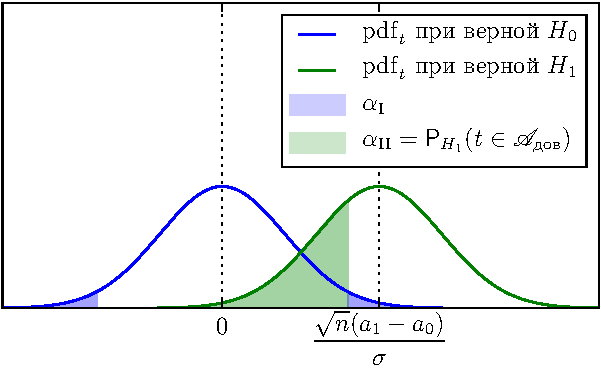
\includegraphics[width=0.5\textwidth]{fig/h0_h1}\caption{Плотности распределения $z$ (неоптимальное разбиение)}
%\end{figure}
%
%
%Чтобы минимизировать $\a_{\mathrm{II}}$, логично определить $\Ascr_{\text{крит}}$
%только на одном хвосте --- с той стороны, где находится альтернатива.
%Помимо этого, по рисунку видно, что минимизировать $\a_{\mathrm{II}}$
%(согласившись на б\'oльшую ошибку первого рода) можно сдвинув вправо
%центр второй плотности, увеличив $n$. Аналогично, чем ${a}_{1}$
%дальше от ${a}_{0}$, тем $\a_{\mathrm{II}}$ меньше.
%
%\begin{figure}[H]
%\centering{}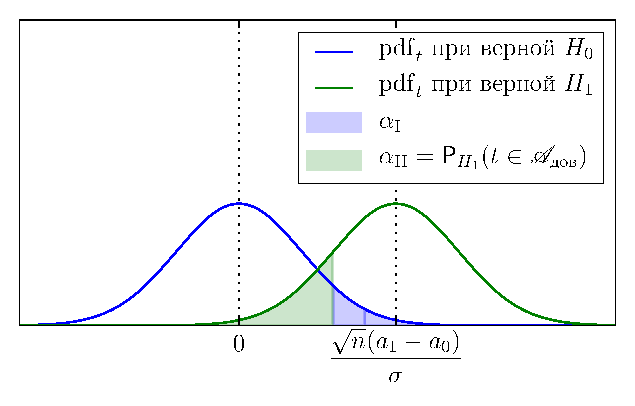
\includegraphics[width=0.5\textwidth]{fig/h0_h1-opt}\caption{Плотности распределения $z$ (оптимальное разбиение)}
%\end{figure}
%
%
%Таким образом, $\Ascr_{\text{крит}}=(C,+\infty)$, $C=z_{1-\a}$.
%
%Разумеется, если ${a}_{_{1}}<{a}_{0}$, то $\Ascr_{\text{крит}}=(-\infty,C),$
%$C=z_{\a}$.
%
%
%\subsection{Односторонний критерий (сложная альтернатива)}
%
%В общем случае, пусть $H_{1}:{a}={a}_{1}\ \forall{a}_{1}>{a}_{0}$;
%тогда по ЗБЧ $\bar{x}-{a}_{0}\to{a}_{1}-{a}_{0}>0$ и $T\to+\infty$.
%Следовательно, чтобы максимизировать величину $\b=\P_{H_{1}}(\mathbf{x}\in\Ascr_{\text{крит}}^{(\a)}),$
%следует разместить $\Ascr$ на правом хвосте плотности: $\Ascr_{\text{крит}}=\left(z_{1-\a},\infty\right)$.
%Для $H_{1}:{a}={a}_{1}\ \forall{a}_{1}<{a}_{0}$ аналогично $\Ascr_{\text{крит}}=\left(-\infty,z_{\a}\right)$.
%
%
%\subsection{Двусторонний критерий}
%
%\begin{comment}
%В случае $T\sim\N(0,1)$, разумно определить $\Ascr_{\text{крит}}$
%<<на хвостах>> графика $\pdf_{\N(0,1)}$ симметрично по обе стороны
%от 0 так, что для $\Ascr_{\text{крит}}=(-\infty,T_{0})\cup(T_{1},\infty)$
%\[
%\a/2=\int_{-\infty}^{T_{0}}\pdf_{\N(0,1)}(y)\d y=\int_{T_{1}}^{+\infty}\pdf_{\N(0,1)}(y)\d y.
%\]
% Иными словами,
%\[
%\a/2=1-\cdf_{\N(0,1)}(T_{1})\implies T_{1}=\cdf_{\N(0,1)}^{-1}(1-\a/2)
%\]
%и аналогично для $T_{0}$.
%\end{comment}
%Пусть $H_{1}:\E\xi={a}_{1}\neq{a}_{0}$; тогда по ЗБЧ $\bar{x}-{a}_{0}\to{a}_{1}-{a}_{0}$
%и $\left|T\right|\xrightarrow[n\to\infty]{}\infty$, откуда $\Ascr_{\text{крит}}=\RR\setminus\left(z_{\a/2},z_{1-\a/2}\right)=\RR\setminus\left(-C,C\right)$,
%где $C=-z_{\a/2}$.
%
%В общем виде, с использованием статистики, критерий может быть определен
%как
%\[
%\varphi(\mathbf{x})=\begin{cases}
%H_{0} & \left|T(\mathbf{x})\right|<C\\
%H_{1} & \left|T(\mathbf{x})\right|\geq C,
%\end{cases}
%\]
%где \emph{критическое значение} $C$ определяется из уравнения $\a=\P(\left|T\right|\geq C)$.
%
%Иногда вместо сравнения значения $T$ с критическим вычисляют \emph{реально
%достигнутый уровень значимости критерия} (<<\emph{$p$-value}>>).
%\begin{defn*}
%\emph{$p$-value }значения статистики $T$ на выборке $\mathbf{x}$
%есть вероятность, взяв выборку из распределения $H_{0}$, получить
%по ней большее отклонение $\left|T(\mathbf{x})\right|$ эмпирического
%от истинного распределения, чем получено по проверяемой выборке:
%\[
%\pv=\a^{*}=\P_{H_{0}}(\left|T\right|\geq\left|T(\mathbf{x})\right|).
%\]
%\begin{comment}
%@xio: TODO: картина с bellcurve, $t_{\mathrm{obs}}$ пойнтом и закрашенной
%вероятностью справа от нее.
%\end{comment}
%
%\end{defn*}
%Значит, критерий может быть задан и как
%\[
%\varphi(\mathbf{x})=\begin{cases}
%H_{0} & \a^{*}>\a\\
%H_{1} & \a^{*}\leq\a.
%\end{cases}
%\]
%
%\begin{rem*}
%$p$-value обратно пропорционален <<существенности>> результата.%
%\begin{comment}
%Иными словами, это мера согласованности $H_{0}$ и выборки.
%\end{comment}
%
%\end{rem*}
%
%\begin{rem*}
%Пусть $\a^{*}=0.05$. Это значит, что в среднем всего лишь 5\% <<контрольных>>
%выборок, удовлетворяющих основной гипотезе, будут обладать большим
%отклонением $\left|T(\mathbf{x})\right|$ по сравнению с тестируемой
%выборкой --- последняя ведет себя не хуже, чем 5\% <<правильных>>
%выборок.
%\end{rem*}
%
%\section{Схема построения критерия с помощью статистики }
%\begin{enumerate}
%\item Фиксируют предположение относительно данных.
%\item Выдвигают $H_{0}$ и $H_{1}$.
%
%\begin{itemize}
%\item $H_{0}$ формулируется согласно замечанию \ref{rem:form-h0}.
%\item $H_{1}$ ставится по смыслу задачи (см. далее).
%\end{itemize}
%\item Выбирают подходящий критерий и статистику $T$.
%\item Фиксируют уровень значимости $\a$.
%\item Строят разбиение $\im T$ с помощью квантилей распределения $T$ (при
%верной $H_{0}$) так, чтобы $\a_{\I}=\a$; положение квантилей выбирают
%из известного поведения статистики при верной $H_{1}$.
%\item Считают значение статистики и принимают решение об отвержении $H_{0}$
%одним из способов:
%\[
%\varphi(\mathbf{x})=\begin{cases}
%H_{0} & \left|T(\mathbf{x})\right|<C\\
%H_{1} & \left|T(\mathbf{x})\right|\geq C,
%\end{cases}\qquad\varphi(\mathbf{x})=\begin{cases}
%H_{0} & \a^{*}>\a\\
%H_{1} & \a^{*}\leq\a.
%\end{cases}
%\]
%\end{enumerate}
%\begin{example*}[Средняя температура в холодильнике]
%Хотят купить холодильник, такой, чтобы температура держалась в окрестности
%0. Известно количество измерений $n=25$ и $\bar{x}=0.7$.
%\begin{enumerate}
%\item Пусть $\xi\sim\N({a},4)$.
%\item Выдвинута $H_{0}:\E\xi={a}_{0}=0$ --- если гипотеза опровергнется,
%то холодильник не купят; $H_{1}:\E\xi={a}_{1}\neq{a}_{0}$.
%\item Поскольку модель нормальная и известная $\sigma^{2}$, выберем статистику
%\ref{sub:E_xi_norm} (<<z-test>>):
%\[
%z=\dfrac{\sqrt{n}\left(\bar{x}-{a}_{0}\right)}{\sigma}\sim\N(0,1)\text{ при верной }H_{0}.
%\]
% Идеальное значение статистики --- 0.
%\item Зафиксируем два уровня значимости: $\a^{(1)}=0.2$ (храним петрушку)
%и $\a^{(2)}=0.01$ (храним дорогую красную икру).
%\item Построим разбиение. Поскольку ${a}_{1}\neq{a}_{0}$, то $\Ascr_{\text{крит}}=\RR\setminus(z_{\a/2},z_{1-\a/2})$.
%Для введенных уровней значимости это означает
%
%\begin{enumerate}
%\item $\Ascr_{\text{крит}}^{(\a^{(1)})}\approx\RR\setminus\left(-1.28,1.28\right)$.
%\item $\Ascr_{\text{крит}}^{(\a^{(2)})}\approx\RR\setminus\left(-2.576,2.576\right)$.
%\end{enumerate}
%\item Посчитаем
%\[
%z(\mathbf{x})=\dfrac{\sqrt{n}\left(\bar{x}-{a}_{0}\right)}{\sigma}=\frac{5(0.7-0)}{2}=1.75.
%\]
%Дальнейшее принятие решения возможно на основании критического значения
%или $p$-value.
%
%\begin{itemize}
%\item По вычислению критического значения:
%
%\begin{itemize}
%\item $z\in\Ascr_{\text{крит}}^{(\a^{(1)})}$, $H_{0}$ отвергается,
%холодильник не покупают.
%\item $z\in\Ascr_{\text{дов}}^{(\a^{(2)})}$, $H_{0}$ не отвергается,
%холодильник, быть может, покупают.
%\end{itemize}
%\item Можно посчитать $p$-value:
%\[
%2\cdot(1-\cdf_{\N(0,1)}(1.75))\approx0.08.
%\]
% Поэтому при уровне значимости $\a^{(1)}=0.2>0.08$ $H_{0}$ отвергается,
%а при $\a^{(2)}=0.01<0.08$ не отвергается.
%\end{itemize}
%\end{enumerate}
%\end{example*}
%
%\begin{example*}[С мышой]
%В одном из рукавов T-образного лабиринта лежит морковка. К развилке
%по лабиринту бежит мышь и 7 раз из 10 поворачивает в направлении морковки.
%На основании этих данных хотим сделать вывод, что мышь чует морковь
%на расстоянии, после чего написать научную статью.
%\begin{itemize}
%\item $\xi\sim\Ber(p)$. Выдвинем гипотезу, что мышь \emph{не} чует морковку,
%$H_{0}:p=p_{0}=0.5$. Поскольку $\E\xi=p$, воспользуемся критерием
%для проверки гипотезы о значении среднего с идеальным значением 0;
%учитывая $\D\xi=p(1-p)$,
%\begin{eqnarray*}
%T & = & \sqrt{n}\frac{\bar{x}-p_{0}}{\sqrt{p_{0}(1-p_{0})}}\tod\N(0,1).\\
% & = & \frac{\sqrt{10}\cdot0.2}{0.5}\approx1.2649\implies p\text{-value}=2\cdot(1-\cdf_{\N(0,1)}(1.2649))\approx0.2.
%\end{eqnarray*}
% Значит, с уровнем значимости $0.2$ гипотеза не отвергается. Хочется
%иметь, конечно, один из стандартных уровней значимости, например $0.1$.
%\item Увеличим мощность критерия, введя альтернативную гипотезу, что мышь
%чует морковку (в предположении, что все мыши любят морковь и к ней
%бегут), $H_{1}:p_{1}>p_{0}$. По \ref{exa:h0-h1}, можем устроить
%односторонний критерий, так что $p$-value теперь 0.1. Однако пользуемся
%асимптотическим критерием при $n=10$.
%\item Воспользуемся точным односторонним критерием со статистикой
%\[
%T:=n\bar{x}=\sum_{i=1}^{n}x_{i}\sim\Bin(n,p_{0})
%\]
% и идеальным значением $np_{0}$. Тогда $T=10\cdot0.7=7$. При уровне
%значимости $\a=0.1$ успешно попадаем в критическую область, вследствие
%чего $H_{0}$ отвергается, и можем публиковаться.
%
%
%\begin{figure}[H]
%\centering{}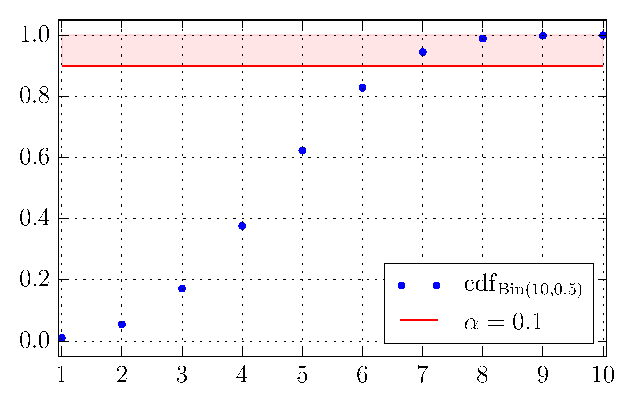
\includegraphics[width=0.5\textwidth]{fig/mouse-bin-cdf}
%\end{figure}
%
%
%\end{itemize}
%\end{example*}
%\begin{rem*}
%Исторически существовало два подхода к проверке гипотез: Фишера (<<significance
%test>>) и Неймана-Пирсона (<<hypothesis testing>>).
%\begin{description}
%\item [{Фишер}] Выдвигается $H_{0}$. Подсчитывается и сообщается точное
%$p$-value. Если результат <<незначительный>>, не делается никаких
%выводов об отвержении $H_{0}$, но делается возможным дополнительный
%сбор данных.
%\item [{Нейман-Пирсон}] Выдвигаются $H_{1},H_{2}$, фиксируются $\a_{\I},\a_{\II}$
%и $n$. На этом основании определяются $\Ascr_{\text{крит}}$
%для каждой гипотезы. Если данные попали в $\Ascr_{\text{крит}}$
%$H_{1}$ --- предпочитается $H_{2}$, иначе $H_{2}$.
%\end{description}
%Современная теория проверки гипотез есть смесь двух этих подходов,
%не всегда консистентная. Вводные курсы по статистике формулируют теорию,
%похожую на significance testing Фишера; при повышенных требованиях
%к математической строгости, пользуются теорией Неймана-Пирсона.
%\end{rem*}
%
%\begin{rem*}[О графике $p$-values]
%Поскольку
%\[
%\a_{\mathrm{I}}\gets\P_{H_{0}}(T\in\Ascr_{\text{крит}})=\P_{H_{0}}(p\text{-value}<\a),
%\]
%то $p$-value по распределению стремятся к $\U(0,1)$ при верной $H_{0}$.
%Это соображение позволяет визуально проверить истинность гипотезы:
%достаточно несколько (много) раз произвести эксперимент, для каждой
%выборки $\bar{x}^{(i)}$ посчитать свой $p$-value, построить
%график и убедиться, что получилась прямая. %
%\begin{comment}
%@xio: проверить
%\end{comment}
%{} Для подсчета мощности $\b=\P_{H_{1}}(\mathbf{x}\in\Ascr_{\text{крит}}^{(\a)})=\P_{H_{1}}(p\text{-value}<\a)$
%считать выборку с параметрами $H_{1}$, а $T$ относительно $H_{0}$.
%\end{rem*}
\chapter{Проверка гипотезы о значении параметра (характеристики)}

\section{Проверка гипотезы о значении мат. ожидания ($t$-критерий)}

$H_{0}:\E\xi={a}={a}_{0}$. Соответствие оценки математического ожидания
гипотезе удобно выражать разницей $\bar{x}-{a}_{0}$ с <<идеальным>>
значением 0. Отнормировав эту разницу, получим статистику, распределение
которой известно.


\subsection{$\protect\D\xi=\sigma^{2}<\infty$}
\begin{prop*}
Пусть $\D\xi=\sigma^{2}<\infty$; тогда используется следующая статистика ($z$-score)
\[
t=z=\sqrt{n}\frac{(\bar{x}-{a}_{0})}{\sigma}\xrightarrow[n\to\infty]{}\N(0,1)
\]
 \end{prop*}
\begin{prop*}
При условии $\xi\sim \N(a,\sigma^2)$,
\[
t=z\sim\N(0,1).
\]
\end{prop*}
\begin{proof}
\[
z=\frac{\bar{x}-{a}_{0}}{\sqrt{\D\bar{x}}}=\sqrt{n}\,\dfrac{\bar{x}-{a}_{0}}{\sigma}\sim\N(0,1).
\]

\end{proof}

%\paragraph{Разбиение}
%\begin{description}
%\item [{$H_{1}:\E\xi\neq{a}_{0}$}] $\Ascr_{\text{крит}}=\RR\setminus\left(z_{\a/2},z_{1-\a/2}\right)$
%\item [{$H_{1}:\E\xi>{a}_{0}$}] $\Ascr_{\text{крит}}=(z_{1-\a},\infty)$
%\item [{$H_{1}:\E\xi<{a}_{0}$}] $\Ascr_{\text{крит}}=(-\infty,z_{\a})$
%\end{description}

\subsection{$\protect\D\xi$ неизвестна}
\label{sect:expect_gen}
\begin{prop*}
Пусть $\D\xi$ неизвестна; тогда используется следующая статистика
\[
t=\sqrt{n-1}\,\frac{\bar{x}-{a}_{0}}{s}=\sqrt{n}\,\frac{\bar{x}-{a}_{0}}{\tilde{s}}\xrightarrow[n\to\infty]{}\N(0,1).
\]
\end{prop*}


Сходимость к нормальному распределению следует из модифицированной теоремы Леви (модифицированная ЦПТ), которая позволяет заменять дисперсию на ее состоятельную оценку с сохранением сходимости к тому же нормальному распределению.


\begin{prop*}
При условии нормальности данных,
\[
t\sim\t(n-1).
\]
\end{prop*}

\begin{comment}
\[
\sum_{i=1}^{n}(x_{i}-\E\xi)^{2}=\sum_{i=1}^{n}(x_{i}-\bar{x})^{2}+n(\bar{x}-\E\xi)^{2}
\]
 --- разложение кв. ф.
\end{comment}



%\paragraph{Разбиение}
%\begin{description}
%\item [{$H_{1}:\E\xi\neq{a}_{0}$}] $\Ascr_{\text{крит}}=\RR\setminus\left(\qnt_{\t(n-1)}(\a/2),\qnt_{\t(n-1)}(1-\a/2)\right)$
%\item [{$H_{1}:\E\xi>{a}_{0}$}] $\Ascr_{\text{крит}}=(\qnt_{\t(n-1)}(1-\a),\infty)$
%\item [{$H_{1}:\E\xi<{a}_{0}$}] $\Ascr_{\text{крит}}=(-\infty,\qnt_{\t(n-1)}\a)$\end{description}
%\begin{rem*}
%При нормальной аппроксимации $\qnt_{\t(n-1)}$ заменить на $\N(0,1)$.
%\end{rem*}

\subsection{Проверка гипотезы о мат.ож. в модели с одним параметром}
\label{sect:expect_one}

Разница с общим случаем состоит в том, что в параметрической модели с одним параметром не нужно оценивать дисперсию. Так как все выражается через этот параметр, то имеем формулу для дисперсии через значение параметра, предполагаемое в нулевой гипотезе.

\paragraph{$z$-критерий для пропорции в модели Бернулли}
Пусть $\xi\sim\Ber(p)$. Поскольку $\E\xi=p$, можно воспользоваться
только что введенной статистикой; учитывая $\D\xi=p(1-p)$, получаем статистику критерия для гипотезы $H_0: p=p_0$:
\[
t=\sqrt{n}\frac{\bar{x}-p_{0}}{\sqrt{p_{0}(1-p_{0})}}\tod\N(0,1).
\]

\paragraph{$z$-критерий для интенсивности потока в модели Пуассона}
Пусть $\xi\sim\Pois(\lambda)$. Поскольку $\E\xi=\lambda$, можно воспользоваться
только что введенной статистикой; учитывая $\D\xi=\lambda$, получаем статистику критерия для гипотезы $H_0: \lambda=\lambda_0$:
\[
t=\sqrt{n}\frac{\bar{x}-\lambda_{0}}{\sqrt{\lambda_{0}}}\tod\N(0,1).
\]


\section{Проверка гипотезы о значении дисперсии в нормальной модели (критерий
$\chi^{2}$)}

Пусть $\xi\sim\N({a},\sigma^{2})$. $H_{0}:\D\xi=\sigma^{2}=\sigma_{0}^{2}$.
Соответствие оценки дисперсии гипотезе удобно выражать отношением
$s^{2}/\sigma_{0}^{2}$ (или $s_{{a}}/\sigma_{0}^{2}$ если ${a}$
известно) с <<идеальным>> значением 1. Домножив на $n$, получим
статистику, распределение которой известно.
%\begin{rem*}[Важное]
%Критерий работает только в нормальной модели и не становится асимптотически
%нормальным в ином случае!
%\end{rem*}

\subsection{$\protect\E\xi={a}<\infty$}
\begin{prop*}
Пусть $\E\xi={a}<\infty$; При условии нормальности данных используется
следующая статистика:
\[
\chi^{2}=n\frac{s_{{a}}^{2}}{\sigma_{0}^{2}}\sim\chi^{2}(n).
\]
\end{prop*}

%\paragraph{Разбиение}
%\begin{description}
%\item [{$H_{1}:\D\xi\neq\sigma_{0}^{2}$}] $\Ascr_{\text{крит}}=\RR_{+}\setminus\left(\qnt_{\chi^{2}(n)}(\a/2),\qnt_{\chi^{2}(n)}(1-\a/2)\right)$
%\item [{$H_{1}:\D\xi>\sigma_{0}^{2}$}] $\Ascr_{\text{крит}}=(\qnt_{\chi^{2}(n)}(1-\a),\infty)$
%\item [{$H_{1}:\D\xi<\sigma_{0}^{2}$}] $\Ascr_{\text{крит}}=(0,\qnt_{\chi^{2}(n)}\a)$
%\end{description}

\subsection{$\protect\E\xi$ неизвестно}
\begin{prop*}
Пусть $\E\xi$ неизвестно. При условии нормальности данных используется
следующая статистика:
\[
\chi^{2}=n\frac{s^{2}}{\sigma_{0}^{2}}=(n-1)\frac{\tilde{s}^{2}}{\sigma_{0}^{2}}\sim\chi^{2}(n-1).
\]
\end{prop*}

%\paragraph{Разбиение}
%\begin{description}
%\item [{$H_{1}:\D\xi\neq\sigma_{0}^{2}$}] $\Ascr_{\text{крит}}=\RR_{+}\setminus\left(\qnt_{\chi^{2}(n-1)}(\a/2),\qnt_{\chi^{2}(n-1)}(1-\a/2)\right)$
%\item [{$H_{1}:\D\xi>\sigma_{0}^{2}$}] $\Ascr_{\text{крит}}=(\qnt_{\chi^{2}(n-1)}(1-\a),\infty)$
%\item [{$H_{1}:\D\xi<\sigma_{0}^{2}$}] $\Ascr_{\text{крит}}=(0,\qnt_{\chi^{2}(n-1)}\a)$\end{description}
\begin{xca*}
$s^{2}=1.44,\bar{x}=55,n=101$. Проверить гипотезу $\sigma_{0}^{2}=1.5$
в нормальной модели.\end{xca*}
\begin{solution}
Воспользуемся статистикой
\[
\chi^{2}=\frac{ns^{2}}{\sigma_{0}^{2}}=101\cdot0.96=96.96.
\]
 <<Идеальные>> значения близки к $\E\xi_{\chi^{2}(100)}=100$, так
что определим критическую область на концах плотности:
\[
\pv/2=\cdf_{\chi^{2}(100)}(96.96)=\mathtt{pchisq(96.96,100)}\approx0.43\implies\pv\approx0.86.
\]

\begin{rem*}
Можно посчитать и по таблицам для нормального распределения. Раз
\[
\frac{\eta_{m}-\E\eta_{m}}{\sqrt{\D\eta_{m}}}\xrightarrow[m\to\infty]{\d}\N(0,1),
\]
 то
\[
\frac{96.96-100}{\sqrt{200}}\approx-0.215\implies\pv/2=\Phi(-0.215)\approx0.415.
\]

\end{rem*}
\end{solution}

\section{Асимптотический критерий для гипотезы о значении параметра на основе MLE}

Если умеем находить $\hat{\th}_{\mathrm{MLE}}$, то по асимптотической
нормальности,
\[
\frac{\hat{\th}_{\mathrm{MLE}}-\E\hat{\th}_{\mathrm{MLE}}}{\sqrt{\D\hat{\th}_{\mathrm{MLE}}}}\tod\N(0,1),
\]
 по асимптотической несмещенности,
\[
\frac{\hat{\th}_{\mathrm{MLE}}-\th}{\sqrt{\D\hat{\th}_{\mathrm{MLE}}}}\tod\N(0,1),
\]
и, учитывая асимптотическую эффективность ($\D\hat{\th}_{\mathrm{MLE}}I_{n}(\th)\xrightarrow[n\to\infty]{}1$),
запишем статистику для $H_0: \th=\th_0$:
\[
t=\left(\hat{\th}_{\mathrm{MLE}}-\th_0\right)\sqrt{I_{n}(\th_0)}\tod\N(0,1).
\]

\textbf{Задание}: построить критерий для гипотезы о значении параметра для распределений Бернулли и Пуассона.

\chapter{Доверительные интервалы}


\section{Мотивация и определение}

Точечные оценки не дают информации о том, насколько (количественно) настоящее значение далеко от оценки.
%Для построенных оценок может понадобиться оценка точности. Так, даже
%состоятельная оценка может не быть в полном смысле <<точной>>: пусть
%$\th_{n}^{*}\toP\th_{0}$; тогда
%\[
%\hat{\th}_{n}'=\begin{cases}
%c & n<N\gg1\\
%\hat{\th}_{n} & \text{иначе}
%\end{cases}
%\]
% все-равно будет, конечно, состоятельной.
%
%$\D\hat{\th}_{n}$ может быть не всегда просто вычислить и использовать.
\begin{defn*}
$\left[b_{1},b_{2}\right]$ --- \emph{доверительный интервал} для
параметра $\theta$ с уровнем доверия $\gamma\in\left[0,1\right]$,
если $\forall\th$
\[
\P(\theta\in\left[b_{1},b_{2}\right])=\gamma,\quad\text{где }b_{1}=b_{1}(\mathbf{x}),b_{2}=b_{2}(\mathbf{x})\text{ --- статистики.}
\]
\end{defn*}
\begin{rem*}
Если выборка из дискретного распределения, то $b_{1},b_{2}$ --- тоже дискретны.
Поэтому наперед заданную точность получить может не получиться; в
таких случаях знак <<$=$>> заменяют <<$\geq$>>. Аналогично с
заменой на <<$\xrightarrow[n\to\infty]{}$>> для асимптотических доверительных интервалов, когда точные получить невозможно или трудоемко.
\end{rem*}

\section{Доверительный интервал для проверки гипотезы о значении параметра}

Зафиксируем $H_{0}:\th=\th_{0}$ и $\gamma=1-\alpha$, где $\a$ играет
роль уровня значимости. По определению доверительного интервала, $\P(\theta\in\left[a_{\gamma}(\mathbf{x}),b_{\gamma}(\mathbf{x})\right])=\gamma.$
Тогда
\[
\P(\theta\in\left[b_1(\mathbf{x}),b_2(\mathbf{x})\right])=
\gamma=1-\a \implies\a=1-\P(\theta\in\left[a_{\gamma}(\mathbf{x}),b_{\gamma}(\mathbf{x})\right])=\P(\th\not\in\left[a_{\gamma}(\mathbf{x}),b_{\gamma}(\mathbf{x})\right])
\]
 и $\Ascr_{\text{крит}}=\RR\setminus\left[b_1(\mathbf{x}),b_2(\mathbf{x})\right].$
Соответственно,
\[
\begin{cases}
\text{отвергаем\ } H_0 \text{, если\ }& \th_0\not\in\left[b_1(\mathbf{x}),b_2(\mathbf{x})\right]\\
\text{не отвергаем\ } H_0 \text{, если\ }& \th_0\in\left[b_1(\mathbf{x}),b_2(\mathbf{x})\right].
\end{cases}
\]
 Вероятность ошибки первого рода равна $\a$, что соответствует определению критерия.
 Заметим, что здесь мы пользуемся общим определением критерия, а не частным случаем, когда критерий строится через статистику критерия.

\section{Доверительные интервалы для математического ожидания и дисперсии
в нормальной модели}
\begin{assumption*}
Пусть $\xi\sim\N({a},\sigma^{2})$.
\end{assumption*}

\subsection{Доверительный интервал для ${a}$}
\begin{itemize}
\item Пусть $\sigma^{2}$ известно. Свяжем ${a}$ с выборкой через статистику критерия \\ $t=\sqrt{n}\frac{(\bar{x}-{a} )}{\sigma}\sim\N(0,1)$:
\[
\gamma=\P(c_{1}<t<c_{2})=\P\left(c_{1}<\sqrt{n}\frac{(\bar{x}-{a})}{\sigma}<c_{2}\right)=\P\left({a}\in\left(\bar{x}-\frac{\sigma c_{2}}{\sqrt{n}},\bar{x}-\frac{\sigma c_{1}}{\sqrt{n}}\right)\right).
\]
 Решений уравнения $\P\left(c_{1}<\sqrt{n}(\bar{x}-{a})/\sigma<c_{2}\right)=\Phi(c_{2})-\Phi(c_{1})=\gamma$
бесконечно много. Чем $\left[c_{1},c_{2}\right]$ короче, тем лучше.
Поскольку $\Phi$ симметрична и унимодальна,
\[
\begin{aligned}c_{1}=-c_{\gamma}\\
c_{2}=c_{\gamma},
\end{aligned}
\quad\text{где }c_{\gamma}=\cdf_{\N(0,1)}^{-1}\left(\gamma+\frac{1-\gamma}{2}\right)=x_{\frac{1+\gamma}{2}}.
\]
\begin{comment}
Картиночка с нормальной плотностью и $\gamma$ в серединке
\end{comment}
{} Наконец,
\[
\P\left({a}\in\left(\bar{x}\pm\frac{\sigma}{\sqrt{n}}c_{\gamma}\right)\right)=\gamma.
\]

\item Пусть $\sigma^{2}$ неизвестно. По аналогии,
\[
\gamma=\P\left(c_{1}<\frac{\sqrt{n-1}(\bar{x}-{a} )}{s}<c_{2}\right)=\P\left({a} \in\left(\bar{x}\pm\frac{c_{\gamma}s}{\sqrt{n-1}}\right)\right),\quad c_{\gamma}=\cdf_{\t(n-1)}^{-1}\left(\frac{1+\gamma}{2}\right)
\]
 и
\[
\P\left({a} \in\left(\bar{x}\pm\frac{\tilde{s}}{\sqrt{n}}c_\gamma\right)\right)=\gamma.
\]
\end{itemize}
\begin{xca*}
Пусть $s^{2}=1.21,\bar{x}=1.9,n=36.$ Построить 95\% доверительный
интервал для $\E\xi$.\end{xca*}
\begin{solution}
\[
c_{\gamma}=\mathtt{qt(0.975,35)}\approx2.03\implies\left(1.9\pm\frac{2.03\cdot\sqrt{1.21}}{\sqrt{35}}\right)=\left(1.52;2.28\right).
\]

\end{solution}

\subsection{Доверительный интервал для $\sigma^{2}$}
\begin{itemize}
\item Пусть ${a}$ известно. Поскольку плотность $\chi^{2}$ становится
все более симметричной с ростом $n$, примем
\[
c_{1}=\cdf_{\chi^{2}(n)}^{-1}\left(\frac{1-\gamma}{2}\right),\ c_{2}=\cdf_{\chi^{2}(n)}^{-1}\left(\frac{1+\gamma}{2}\right).
\]
 Тогда
\[
\P\left(c_{1}<\frac{ns_{{a}}^{2}}{\sigma ^{2}}<c_{2}\right)=
\gamma\iff\P\left(\sigma ^{2}\in\left(\frac{ns_{{a}}^{2}}{c_2},\frac{ns_{{a}}^{2}}{c_1}\right)\right)=\gamma.
\]

\item Пусть ${a}$ неизвестно. Тогда аналогично
\[
\P\left(\sigma ^{2}\in\left(\frac{ns^{2}}{c_2},\frac{ns^{2}}{c_1}\right)\right)=\gamma,
\]
где
\[
c_{1}=\cdf_{\chi^{2}(n-1)}^{-1}\left(\frac{1-\gamma}{2}\right),\ c_{2}=\cdf_{\chi^{2}(n-1)}^{-1}\left(\frac{1+\gamma}{2}\right).
\]

\end{itemize}

%\begin{defn*}
%Случайная величина $g(x_{1},\ldots,x_{n},\th)$ называется \emph{центральной
%статистикой параметра} $\th$, если
%\begin{enumerate}
%\item Её распределение (<<центральное распределение>>) не зависит от распределения
%$\th$.
%\item $G_{n}$ (функция распределения центрального распределения) непрерывна.
%\item $\forall z_{1},z_{2}$ и $\Pcal_{\th}$-почти всюду
%\[
%z_{1}<g(x_{1},\ldots,x_{n},\th)<z_{2}
%\]
% монотонно разрешимо относительно $\th$, т.е.
%\[
%\exists f_{1},f_{n}:f_{1}(x_{1},\ldots,x_{n},\th,z_{1},z_{2})<\th<f_{2}(x_{1},\ldots,x_{n},\th,z_{1},z_{2}).
%\]
%
%\end{enumerate}
%\end{defn*}
%Рассмотрим всегда разрешимое
%\begin{eqnarray*}
%\gamma & = & G_{n}(z_{2})-G_{n}(z_{1})=\P(z_{1}<g(x_{1},\ldots,x_{n},\th)<z_{2})\\
% & = & \P(\underbrace{f_{1}(z_{1},z_{2},x_{1},\ldots,x_{n})}_{c_{1}}<\th<\underbrace{f_{2}(z_{1},z_{2},x_{1},\ldots,x_{n})}_{c_{2}}).
%\end{eqnarray*}
%



%\end{document}
\section{Асимптотический доверительный интервал для математического ожидания
в модели с конечной дисперсией}

Если модель неизвестна, но известно, что $\D\xi<\infty$, можно построить
доверительный интервал для $\E\xi={a}$, не задавая параметрическую модель.
Пусть $\left\{ x_{i}\right\} $
$\iid$, тогда
\[
t=\frac{\sqrt{n}\left(\bar{x}-{a}\right)}{\sigma}\xrightarrow[n\to\infty]{}\N(0,1).
\]
 Если заменить $\sigma$ на ее состоятельную оценку ($s$), то по модифицированной теореме Леви (будет у Владимира Викторовича в след.году) сходимость не испортится. Тогда
\[
\P\left(\E\xi\in\left(\bar{x}\pm\frac{sc_{\gamma}}{\sqrt{n}}\right)\right)\xrightarrow[n\to\infty]{}\gamma,\quad c_{\gamma}=\cdf_{\t(n-1)}^{-1}\left(\frac{1+\gamma}{2}\right).
\]

Все это так же, как было в разделе \ref{sect:expect_gen}.

Аналогично разделу \ref{sect:expect_one}, доверительные интервалы можно улучшить (сделать большее точными, т.е. вероятность попадания в них ближе к $\gamma$ при фиксированном $n$) в параметрической модели, если вместо независимой оценки дисперсии использовать оценку, полученную на основе оценок параметров. Разница в том, что там можно было использовать значение параметра, взятое из гипотезы, а в доверительных интервалах  придется подставлять оценки (или решать нелинейные неравенства, см. следующий раздел).
%Альтернативно замену $\sigma$ на $s$ можно обосновать по теореме
%Слуцкого.
%\begin{claim*}[Слуцкий]
%Если $\xi_{n}\tod\xi,\ \eta_{n}\toP c$, то $\xi_{n}+\eta_{n}\tod\xi+c$
%и $\xi_{n}\eta_{n}\tod c\xi$.
%\end{claim*}
%Используя тот факт, что $s\toP\sigma$, запишем
%\[
%\P\left(c_{1}<\frac{\sqrt{n}\left(\bar{x}-{a}\right)}{\sigma}\frac{\sigma}{s}<c_{2}\right)\xrightarrow[n\to\infty]{}\Phi(c_{2})-\Phi(c_{1}).
%\]

\section{Асимптотический доверительный интервал для параметра на основе MLE}

В точности, как было при проверке гипотез,
\[
T=\left(\hat{\th}_{\mathrm{MLE}}-\th\right)\sqrt{I_{n}(\th)}\tod\N(0,1).
\]
 Чтобы по аналогии с предыдущим выразить $\th$ в $\P(c_{1}<T<c_{2})=\P(\left|T\right|<c_{\gamma})=\gamma$,
необходимо знать зависимость $I_{n}(\th)$ от  $\th$. Для $\Pois$ и $\Ber$
разрешение неравенства относительно $\th$ эквивалентно решению неравенства для квадратичного полинома. %
\begin{comment}
@xio: FIXME: Не симметрично; но для $\hat{\lambda}$ не будет $<0$;
для $\hat{p}\in[0,1]$.
\end{comment}


В общем случае, можно вместо $\th$ в $I_{n}(\th)$ подставить $\hat{\th}_{\mathrm{MLE}}$
(при $n\to\infty$ это не должно сильно испортить дело), откуда
\begin{eqnarray}
\P\left(-c_{\gamma}<\left(\hat{\th}_{\mathrm{MLE}}-
\th\right)\sqrt{I_{n}(\hat{\th}_{\mathrm{MLE}})}<c_{\gamma}\right)\to
\gamma\iff \\
\P\left(\th\in\left(\hat{\th}_{\mathrm{MLE}}\pm\frac{c_{\gamma}}{\sqrt{I_{n}(\hat{\th}_{\mathrm{MLE}})}}\right)\right)\to\gamma,
\end{eqnarray}
 где
\[
T\tod\N(0,1)\implies c_{\gamma}=\cdf_{\N(0,1)}^{-1}\left(\frac{1+\gamma}{2}\right).
\]

\begin{example*}
$\xi\sim\Pois(\lambda)$. В разделе~\ref{exa:mle-pois} получали: $\hat{\lambda}_{\mathrm{MLE}}=\bar{x}$ и
$I_{n}(\lambda)=n/\lambda$ и $I_{n}(\hat\lambda)=n/\bar{x}$,
откуда
\[
\P\left(\lambda\in\left(\bar{x}\pm c_\gamma\frac{\sqrt{\bar{x}}}{\sqrt{n}}\right)\right) \xrightarrow[n\to\infty]{}\gamma.
\]
 %
\begin{comment}
@xio: FIXME: для $\E\xi$, $\sqrt{\bar{x}}=S\because\widehat{\D\xi}=\bar{x}=\hat{\lambda}$?
\end{comment}

\end{example*}
\begin{rem*}
Этот доверительный интервал не очень хорош, потому что может включать значения меньше 0.
\end{rem*}

\begin{example*}
$\xi\sim\Ber(p)$. $p=\E\xi$. $\hat{p}=\bar{x}$, откуда
\[
\P\left(p\in\left(\hat{p}\pm c_{\gamma}\frac{\sqrt{\hat{p}(1-\hat{p})}}{\sqrt{n}}\right)\right)\xrightarrow[n\to\infty]{}\gamma.
\]

\begin{rem*}
Этот доверительный интервал не очень хорош, потому что не обязательно принадлежит
$\left[0,1\right]$.
\end{rem*}
\end{example*}

\textbf{Задание}: Построить хорошие доверительные интервалы в моделях Бернулли и Пуассона, решив неравенства с квадратными уравнениями.

\textbf{Задание}: Построить доверительный интервал для параметра $\lambda$ экспоненциального распределения $\Exp(\lambda)$.


\section{Использование $\SE$ для проверки гипотез и построения доверительных интервалов}

Пусть оценка $\hat{\th}_{n}$ имеет (асимптотически) нормальное распределение и является асимптотически несмещенной. Тогда
 доверительный интервал уровня $\gamma$ для $\th$ (т.е. такой интервал, в котором лежит $\gamma$ всех значений величины)
задается как
\[
\hat{\th}_{n}\pm c_{\gamma}\sqrt{\D\hat{\th}_{n}},
\]
где $c_{\gamma}$ --- $(\gamma+1)/2$-квантиль стандартного нормального распределения.
К примеру, для $\N(0,1)$ и 95\%-квантили это был бы интервал$(-1.96;1.96)$, а так нужно передвинуть его на
среднее и растянуть на корень из дисперсии.

Но стандартное отклонение $\sqrt{\D\hat{\th}_{n}}$ распределения
$\hat{\th}_{n}$ можно оценить как $\SE$ (standard error, стандартная ошибка). Значит, доверительный интервал
будет иметь вид
\[
\hat{\th}_{n}\pm c_{\gamma}\SE.
\]

Аналогично, статистика критерия $H_0: \th = \th_0$ будет иметь вид
\[
t = (\hat{\th}_{n} - \th_0)/\SE(\hat{\th}_{n}),
\]
которая имеет асимптотически нормальное распределение $\N(0,1)$ с `идеальным' значение в нуле.

Заметим, что $\SE$ играет роль `сигмы' распределения оценки.
 %
\begin{comment}
Чтобы сходимость оставалась верной, даже если подставляем оценку,
нужна состоятельность.
\end{comment}


\chapter{Критерии проверки гипотезы о согласии с видом распределения}
\section{Критерий $\chi^{2}$}

По выборке возможно проверить гипотезу о виде распределения случайной
величины, реализацией которой является выборка.
Для проверки гипотезы согласия с видом произвольного \emph{дискретного}
распределения используется асимптотический \emph{критерий $\chi^{2}$
(<<chi-squared test for goodness of fit>>).}

\subsection{Распределение с известными параметрами}

Пусть
\[
H_{0}:\Pcal=\Pcal_{0},\text{ где }\Pcal_{0}:\begin{pmatrix}x_{1}^{*} & \dots & x_{k}^{*}\\
p_{1} & \dots & p_{k}
\end{pmatrix}.
\]
 Сгруппируем $\mathbf{x}$; каждому $x_{i}^{*}$ сопоставим \emph{эмпирическую}
абсолютную частоту $\nu_{i}$; тогда $np_{i}$ --- \emph{ожидаемая}
абсолютная частота.

В качестве меры расхождения между эмпирическим и генеральным распределением
рассматривается величина
\[
\sum_{i=1}^{k}c_{i}\left(\frac{\nu_{i}}{n}-p_{i}\right)^{2},\quad c_{i}=\frac{n}{p_{i}},
\]
 откуда записывается статистика критерия
\[
T=\sum_{i=1}^{k}\frac{(\nu_{i}-np_{i})^{2}}{np_{i}}
\]
 с `идеальным' значением 0 (следовательно, критическая область только справа).
\begin{claim*}
$T\tod\chi^{2}(k-1)$.
\end{claim*}

%\paragraph{Разбиение}
%
%$\Ascr_{\text{крит}}=\left(\qnt_{\chi^{2}(k-1)}(1-\a),\infty\right)$
%--- гипотеза отвергается, если расстояние между предполагаемым и наблюдаемым
%распределениями большое.

\begin{defn*}
Критерий \emph{применим}, если $\a_{\mathrm{I}}=\a$ или $\a_{\mathrm{I}}\approx \a$ с достаточной степенью точности.%
\begin{comment}
@xio: так?
\end{comment}
\begin{comment}
$n\downarrow\implies$ не применим
\end{comment}
\end{defn*}
\begin{rem*}
Поскольку критерий асимптотический, с достаточной (тому, кто дает такие рекомендации) степенью точностью
он применим в случае, если
\begin{enumerate}
\item $n\geq50$;
\item $np_{i}\geq5.$
\end{enumerate}
\end{rem*}

\begin{rem*}
Если условие $np_{i}\geq5$ не выполняется, следует объединить состояния,
например, с краев или слева направо; если в хвосте оказалось $<5$,
то следует присоединить к последнему.\end{rem*}

\begin{rem*}
Почему бы не подстраховаться и не объединить состояния так, чтобы было >10? Ответ: теряем в мощности. \\
\textbf{Задание} Привести пример, демонстрирующий потерю мощности.
\end{rem*}


\begin{example*}[С монеткой]
Пусть $n=4040$, $\#\mathrm{H}=2048,\ \#\mathrm{T}=1092$. Проверим
$H_{0}:\Pcal=\Ber(0.5)$ с $\a=0.1$. Условия критерия выполняются,
поэтому посчитаем
\[
T=\frac{(2048-2020)^{2}}{2020}+\frac{(1092-2020)^{2}}{2020}=\frac{28^{2}+28^{2}}{2020}\approx0.78,
\]
откуда
\[
p\text{-value}=1-\cdf_{\chi^{2}(1)}(0.78)\approx0.38.
\]
 $0.38>0.1$, значит $H_{0}$ не отвергается.\end{example*}
\begin{rem*}
Если нужно подстраховаться от подгонки (искусственно составленных под гипотезу выборок), то критическую область можно выбрать с двух сторон, слева и справа. Например, чтобы отверглась гипотеза о $p=0.5$ для альтернирующей (и явно не
случайной) последовательности $\mathbf{x}=(0,1,0,1,\ldots)$ имеет
$T=0$.
Однако, если мы не подозреваем данные в обмане, то так не делают.
\begin{comment}
@xio: вставить про разные виды графиков: не случайная выборка ---
выгнута вверх, не равномерная --- вниз?
\end{comment}

\end{rem*}



%\begin{xca*}
%$n=100$,
%\[
%\begin{pmatrix}\diamondsuit & \heartsuit & \clubsuit & \spadesuit\\
%20 & 30 & 10 & 40
%\end{pmatrix}.
%\]
% Проверить гипотезу, что колода полная.\end{xca*}
%\begin{solution}
%$H_{0}:\Pcal_{\xi}=\U(1/4)$. Поскольку речь идет о согласии с дискретным
%не параметризованным распределением, напрямую воспользуемся критерием
%$\chi^{2}$. Раз все $np_{i}=100\cdot1/4=25,$
%\[
%\chi^{2}=\sum_{i=1}^{k}\frac{(\nu_{i}-np_{i})^{2}}{np_{i}}=1+1+\frac{15^{2}}{25}+\frac{15^{2}}{25}=2+2\cdot9=20.
%\]
% Так как $\chi^{2}\sim\chi^{2}(k-1)=\chi^{2}(3)$ со средним 3, и
%<<идеальное>> значение 0, определим критическую область в правом
%конце плотности. Из этих соображений
%\[
%\pv=1-\cdf_{\chi^{2}(3)}(20)=1-\mathtt{pchisq(20,3)}\approx0.00017.
%\]
%
%\end{solution}

\subsection{Распределение с неизвестными параметрами}

В случае сложной гипотезы $\Pcal\in\left\{ \Pcal(\thb)\right\} _{\thb\in\Theta}$,
$\thb=\left(\th_{1},\ldots,\th_{r}\right)^{\T},$ следует найти оценку
$\hat{\thb}_{\mathrm{MLE}}$ %(или $\hat{\thb}:\hat{\thb}\to\hat{\thb}_{\mathrm{MLE}}$)
по методу максимального правдоподобия. При подстановке оценок вместо
истинных параметров критерий становится консервативным. Чтобы этого
избежать, необходимо сделать поправку на количество параметров ---
отнять $r$. Что приятно, одна и та же поправка работает для всех
распределений; в этом случае,
\[
T =  \sum_{i=1}^{k}\frac{(\nu_{i}-np_{i}(\hat\thb_{\mathrm{MLE}}))^{2}}{np_{i}}
\tod\chi^{2}(k-r-1).
\]

Важно: параметр можно считать известным, только если его значение выбрано без знания, какая получилась выборка.

\paragraph{Оценки по методу минимума хи-квадрат}
Предельное распределение статистики критерия не поменяется, если вместо оценки максимального правдоподобия подставить любую другую оценка с тем же предельным распределением. Рассмотрим оценки по минимуму хи-квадрат:
\[
\thb_{\mathrm{minChiSq}} =
\arg \min_{\thb} \sum_{i=1}^{k}\frac{(\nu_{i}-np_{i}(\thb))^{2}}{np_{i}}
\tod\chi^{2}(k-r-1).
\]

Утверждение (без доказательства) заключается в том, что в условиях регулярности оценки, полученные по методу максимального правдоподобия, эквивалентны оценкам, полученным по методу минимума хи-квадрат. Таким образом, в критерии хи-квадрат можно использовать статистику в виде
\[
T =  \min_{\thb} \sum_{i=1}^{k}\frac{(\nu_{i}-np_{i}(\thb))^{2}}{np_{i}}
\tod\chi^{2}(k-r-1).
\]


%\begin{xca}
%60 человек купило подарок сразу, 10 со второго раза, 20 с третьего,
%10 с четвертого:
%\[
%\begin{pmatrix}0 & 1 & 2 & 3\\
%60 & 10 & 20 & 10
%\end{pmatrix}.
%\]
% Проверить гипотезу о том, что это выборка из геометрического распределения.\end{xca}
%\begin{solution}
%$H_{0}:\Pcal_{\xi}=\Geom(p)$. Воспользуемся критерием $\chi^{2}$
%для параметризированного распределения $\Geom(\hat{p}_{\MLE}).$
%
%Найдем
%\[
%\hat{p}_{\MLE}=\argmax_{p}\log\L(\mathbf{x};p)\Longleftarrow\frac{\d}{\d p}\log\L(\mathbf{x};\hat{p}_{\MLE})=0.
%\]
% Так как $\pdf_{\Geom(p)}(k)=(1-p)^{k}p$,
%\begin{eqnarray*}
%\log\L(\mathbf{x};p) & = & \log\prod_{k=1}^{n}(1-p)^{k}p=\log(1-p)^{n\bar{x}}p^{n}=n\bar{x}\log(1-p)+n\log p\\
% & = & n(\bar{x}\log(1-p)+\log p)
%\end{eqnarray*}
% откуда
%\[
%\frac{\d}{\d p}\log\L(\mathbf{x};p)=n\left(-\frac{\bar{x}}{1-p}+\frac{1}{p}\right)=0\iff1-p-p\bar{x}=0\iff p=\frac{1}{1+\bar{x}}.
%\]
% Учитывая
%\[
%\bar{x}=0.1+2\cdot0.2+3\cdot0.1=0.8,
%\]
% найдем
%\[
%\hat{p}_{\MLE}=\frac{1}{1+0.8}\approx0.55.
%\]
%
%
%Посчитаем статистику $\chi^{2}$, найдя соответствующие $p_{i}$:
%\[
%p_{0}=\P_{\Geom(0.55)}(0)=0.55,\quad p_{1}\approx0.26,\quad p_{2}\approx0.11,\quad p_{3}\approx0.09.
%\]
% Тогда
%\[
%\chi^{2}=\sum_{i=1}^{k}\frac{\left(\nu_{i}-np_{i}\right)^{2}}{np_{i}}=\frac{25}{55}+\frac{16^{2}}{26}+\frac{81}{11}+\frac{1}{9}\approx17.77.
%\]
% Наконец, поскольку $\chi^{2}\xrightarrow[n\to\infty]{}\chi^{2}(k-r-1)$,
%\[
%\pv=1-\cdf_{\chi^{2}(2)}(17.77)\approx0.00014.
%\]
%\end{solution}


%\section{Согласие с нормальным распределением по $\chi^{2}$}
%
%Для проверки гипотезы $H_{0}:\Pcal_{\xi}=\N(a,\sigma^{2})$ также
%можно воспользоваться статистикой критерия $\chi^{2}$ для сложной
%гипотезы. В этом случае, нужно дискретизировать нормальное распределение,
%так, что
%\[
%\Pcal_{0}=\begin{pmatrix}x_{1}^{*} & \dots & x_{k}^{*}\\
%p_{1}(\hat{\thb}) & \dots & p_{k}(\hat{\thb})
%\end{pmatrix},\quad\hat{\thb}=\hat{\thb}_{\MLE}.
%\]
%Тем не менее, нужно иметь в виду две теоретических неточности:
%\begin{enumerate}
%\item Построение $\Pcal_{0}$ происходит случайно, в результате объединения
%элементов выборки после того, как она получена.
%\item Оценка параметров $\hat{\thb}_{\MLE}$ должна быть посчитана для $\Pcal_{0}$,
%а не для исходного (нормального) распределения --- не $\bar{x},s^{2}$.
%Однако на практике на этот момент не обращают внимания.
%\end{enumerate}
%Существует два возможных способа дискретизации:
%\begin{enumerate}
%\item Гистограмма: одинаковые интервалы, но разные вероятности.
%\item Неравные интервалы с равными вероятностями. %
%\begin{comment}
%@xio: это правильный алгоритм? mean?
%\end{comment}
%
%
%\begin{lyxcode}
%N~<-~length(xs)
%
%xs~<-~sort(xs)
%
%probs~<-~pnorm(xs,~mean=mean(xs),~sd=sd(xs))
%
%i~<-~1;~j~<-~i+1
%
%while~(N~{*}~(probs{[}j{]}~-~probs{[}i{]})~<~5)~\{
%
%~~j~<-~j+1
%
%\}
%
%mean(xs{[}i:j{]})~~\#~our~$x_{1}^{*}$;~$n_{1}=j-i+1$
%\end{lyxcode}
%
%Этот способ разбиения предпочтителен, потому что:
%\begin{itemize}
%\item Можно разбить максимально часто --- так, чтобы $np_{i}=5\ \forall i$,
%следовательно и мощность будет максимальна.
%\item Он оказывается точнее первого на практике.
%\item Получается единственное $p$-value.\end{itemize}
%\begin{rem*}
%Следует иметь в виду, что этот способ не годится для непрерывных,
%но плохо дискретизированных данных.
%\end{rem*}
%\end{enumerate}

\chapter{Критерий Колмогорова-Смирнова согласия с видом распределения}


\section{Произвольное абсолютно непрерывное распределение}

$H_{0}:\xi\sim\Pcal=\Pcal_{0}$.
\begin{claim*}
Для проверки гипотезы согласия с видом произвольного \emph{абсолютно
непрерывного }распределения с известными параметрами используется
точный критерий Колмогорова-Смирнова со следующей статистикой:
\[
D_{n}=\sup_{x\in\mathbf{x}}\left|\widehat{\cdf}_{n}(x)-\cdf_{0}(x)\right|,
\]
 где $\cdf_{0}$ --- функция распределения $\Pcal_{0}$ нулевой гипотезы. Распределение $D_{n}$, оно разное для разных $n$, но не зависит от распределения.

%\begin{comment}
Распределение не зависит от $\cdf_{0}$, так как любое распределение можно привести, например, к равномерному, монотонным преобразованием:
для любой $\cdf_{0}$  верно $\cdf_{0}^{-1}(\xi)\sim\U(0,1)$,
как будто, мы проверяем гипотезу $H_0: \cdf_{0}^{-1}(\xi)\sim\U(0,1)$.
%Значение супремума при этом не меняется, значит, не
%зависит от $F_{0}$.
%\end{comment}


Альтернатива только одна: $H_{1}:\xi\not\sim\Pcal_{0}$; $\Ascr_{\text{крит}}=(\qnt_{\text{K-S}}(1-\a),\infty).$\end{claim*}
\begin{rem*}
Критерий является \emph{точным}, не асимптотическим. Значит, им можно
пользоваться и при маленьких объемах выборки (мощность, при этом,
останется низкой все-равно).
\end{rem*}

\begin{rem*}
$\sqrt{n}\sup_{x}\left|\widehat{\cdf}_{n}(x)-\cdf_{0}(x)\right|\tod\Pcal_{\mathrm{K.S.}}$,
где $\Pcal_{\mathrm{K.S.}}$ --- распределение Колмогорова. Это удобно тем, что распределение такой статистики критерия не зависит от $n$. Значит,
при больших объемах выборки для такой статистики критерия можно пользоваться
таблицами распределения Колмогорова.\end{rem*}

%\end{document}
%\begin{xca*}
%Проверить гипотезу, что $\mathbf{x}=\left(0.1,0.2,0.4,0.3,0.1\right)$
%есть выборка из $\U[0,1]$.\end{xca*}
%\begin{solution}
%$D_{n}=0.6$, $\pv\approx0.05$ (по таблицам или компьютером). Таким
%образом, при $\a>0.05$ гипотеза отвергается, при $\a<0.05$ --- нет.
%\begin{lyxcode}
%>~ks.test(c(0.1,0.2,0.4,0.3,0.1),~'punif')
%
%
%
%~~~~~~~~One-sample~Kolmogorov-Smirnov~test
%
%
%
%data:~~c(0.1,~0.2,~0.4,~0.3,~0.1)
%
%D~=~0.6,~p-value~=~0.05465
%\end{lyxcode}
%\end{solution}
%\begin{rem*}
%Критерий Колмогорова-Смирнова консервативный --- значение $p$-value
%завышено. Поэтому если гипотеза отвергается, то наверняка.
%\end{rem*}

%\section{Нормальное распределение}
%
%Пусть $H_{0}:\Pcal_{\xi}\in\left\{ \N({a},\sigma^{2})\right\} $.
%Как известно, критерий Колмогорова-Смирнова используется для непрерывных
%непараметрических распределений. Им можно воспользоваться и для данной
%$H_{0}$, если вместо ${a},\sigma^{2}$ подставить соответствующие
%оценки --- в таком случае критерий будет консервативным. По аналогии
%с $\chi^{2}$ хотелось бы сделать поправку на количество параметров
%--- такая поправка осуществляется путем моделирования распределения
%тестовой статистики. Для $\N({a},\sigma^{2})$ и $\Exp(\lambda)$
%получаем распределение $D_{n}$, не зависящее от параметров (так что
%поправку можно делать вне зависимости от параметров; к примеру, $\N({a},\sigma^{2})$
%можно привести к $\N(0,1)$ непрерывным преобразованием):
%\begin{description}
%\item [{Критерий~Бартлетта}] есть критерий Колмогорова-Смирнова для $H_{0}:\Pcal_{\xi}=\Exp(\lambda)$.%
%\begin{comment}
%@xio: FIXME: что $\Exp$ делает в этом разделе
%\end{comment}
%
%\item [{Критерий~Лиллиефорса\footnote{Lilliefors.}}] для проверки $H_{0}:\Pcal_{\xi}=\N({a},\sigma^{2})$
%считается статистикой $D_{n}$ c $\cdf_{0}(x)=\cdf_{\N(\bar{x},s^{2})}(x)$,
%сходящейся к распределению Лиллиефорса (Колмогорова-Смирнова с учетом
%подстановки оценок).
%\item [{Критерий~Шапиро-Уилка}] $T\approx\rho^{2}$, т.е. ведет себя примерно
%как квадрат коэффициента корреляции на normal probability plot.\end{description}
%\begin{rem*}
%Распределения в случае критерия Лиллиефорса были получены путем
%моделирования.\end{rem*}
%\begin{example*}
%В R:
%\begin{lyxcode}
%>~require('nortest')
%
%>~xx~<-~rt(1000,~df=20)
%
%>~lillie.test(xx)
%
%~~~~~~~~Lilliefors~(Kolmogorov-Smirnov)~normality~test
%
%data:~~xx
%
%D~=~0.023412,~p-value~=~0.2032
%
%>~shapiro.test(xx)
%
%~~~~~~~~Shapiro-Wilk~normality~test
%
%data:~~xx
%
%W~=~0.99669,~p-value~=~0.03409
%
%
%\end{lyxcode}
%\end{example*}
%
%\chapter{Критерий типа $\omega^{2}$}
%\begin{defn*}
%Статистика
%\[
%Q=n\int_{\RR}\left(\cdf_{n}(x)-\cdf_{0}(x)\right)^{2}w(x)\d\cdf_{0}(x),
%\]
% где $w(x)$ --- весовая функция.\end{defn*}
%\begin{rem*}
%Статистика может быть проинтерпретирована как площадь разницы между
%соответствующими функциями распределения.\end{rem*}
%\begin{description}
%\item [{Cramer~von~Mises}] $Q$ с $w\equiv1$.
%\item [{Anderson-Darling}] $Q$ с
%\[
%w(x)=\frac{1}{\cdf_{0}(x)(1-\cdf_{0}(x))}.
%\]
%\end{description}
%\begin{rem*}
%Весовая функция критерия Anderson-Darling присваивает большой вес
%значениям на хвостах распределения, поэтому сам критерий является
%мощным против разницы на хвостах, но и менее мощным при сдвиге.
%\end{rem*}
%
%\begin{rem*}
%Все эти критерии точны.
%\end{rem*}
%
%\begin{rem*}
%Распределение статистики в каждом случае не зависит от $\cdf_{0}$
%и все эти критерии состоятельные против любой альтернативы, поэтому
%не очень мощные.%
%\begin{comment}
%@xio: Какие альтернативы важны? AD --- отличия на хвостах. KS-test,
%$t_{+},t_{-},t=\max(t_{+},t_{-})$. $t_{+}\rightsquigarrow F_{n}(x)>F_{0}(x),\ t_{-}\rightsquigarrow F_{n}(x)<F_{0}(x).$
%Пусть $F_{0}$ отличается от $\cdf_{\xi}$ только сдвигом, т.е. $\xi=\xi_{0}+a$.
%тогда $t_{+}=a,\ t_{-}=0$. <картиночка>
%
%Пусть $\xi=c\xi_{0}$, тогда <картиночка>
%\end{comment}
%
%\end{rem*}
%
%\begin{rem*}
%Из всех тестов для тестирования согласия с нормальным распределением
%наибольшей мощностью при любых объемах выборки почти всегда обладает
%Shapiro-Wilk, см. \url{http://www.de.ufpb.br/~ulisses/disciplinas/normality_tests_comparison.pdf}
%\end{rem*}

\chapter{Визуальное определение согласия с распределением}


\section{P-P plot}
\begin{defn*}
\emph{P-P plot} есть график
\[
\left\{ \left(\cdf_{0}(x_{i})+\frac{1}{2n},\widehat{\cdf}_{n}(x_{i})\right)\right\} _{i=1}^{n}.
\]
\end{defn*}
\begin{example*}
В R:
\begin{lyxcode}
pp.plot~<-~function(xs,~cdf.0=pnorm,~n.knots=1000)~\{

~~knots~<-~seq(min(xs),~max(xs),~length.out=n.knots)

~~plot(cdf.0(knots),~ecdf(xs)(knots))

~~abline(0,~1)

\}
\end{lyxcode}
\end{example*}

\section{Q-Q plot}
\begin{defn*}
\emph{Q-Q plot} есть график
\[
\left\{ \left(x_{i},\cdf_{0}^{-1}\left(\widehat{\cdf}_{n}(x_{i})+\frac{1}{2n}\right)\right)\right\} _{i=1}^{n}.
\]

\end{defn*}

\begin{defn*}
Частный случай Q-Q plot для $\cdf_{0}^{-1}=\cdf_{\N(0,1)}^{-1}$ называется
\emph{normal probability plot}.\end{defn*}
\begin{example*}
В R:
\begin{lyxcode}
qq.plot~<-~function(xs,~qf.0=qnorm,~n.ppoints=1000)~\{

~~qs~<-~ppoints(n.ppoints)

~~plot(qf.0(qs),~unname(quantile(xs,~probs=qs)))

~~abline(mean(xs),~sd(xs))

\}
\end{lyxcode}
\end{example*}
\begin{rem*}
Если $\hat{\Pcal}_{n}\to\Pcal_{\xi}$, то оба графика будут стремиться
к $y=x$. Референсной прямой normal probability plot будет $y=\widehat{\D\xi}\cdot x+\widehat{\E\xi}$.
\end{rem*}

\begin{rem*}
Больше о различии Q-Q и P-P plots, см. \url{http://v8doc.sas.com/sashtml/qc/chap8/sect9.htm}
\end{rem*}

\begin{rem*}
Различные интерпретации параметров распределения по Q-Q plot можно
посмотреть в интерактивном приложении: \url{https://xiongge.shinyapps.io/QQplots/}
\end{rem*}

%\chapter{Гипотеза о равенстве распределений}
%
%$H_{0}:\Pcal_{\xi_{1}}=\Pcal_{\xi_{2}}.$
%
%Возможно рассматривать два случая:
%\begin{description}
%\item [{Независимые~выборки}] Две группы индивидов, на которых измеряется
%один и тот же признак. Формально: пусть $\zeta\in\left\{ 1,2\right\} $
%--- номер группы, $\xi$ --- признак. Тогда $\xi_{1}\sim\Pcal_{\xi\mid\zeta=1},\ \xi_{2}\sim\Pcal_{\xi\mid\zeta=2}$
%и $\xi_{1}\indep\xi_{2}$. В этом случае выборка имеет вид
%\[
%\left(\left(x_{1},x_{2},\ldots,x_{n_{1}}\right),\left(y_{1},y_{2},\ldots,y_{n_{2}}\right)\right)
%\]
%или
%
%
%\begin{center}
%\begin{tabular}{ccccccc}
%\toprule
%$\xi$ & $x_{1}$ & $\dots$ & $x_{n_{1}}$ & $y_{1}$ & $\dots$ & $y_{n_{2}}$\tabularnewline
%\bottomrule
%\end{tabular}
%\par\end{center}
%
%
%то есть одному признаку сопоставлено $n_{1}+n_{2}$ индивидов.
%
%\item [{Зависимые~выборки}] Одна группа индивидов, на каждом из которых
%измеряются две характеристики (либо же <<до>> и <<после>>). В
%этом случае выборка имеет вид
%\[
%\left(\left(x_{1},y_{1}\right),\ldots,(x_{n},y_{n})\right)
%\]
% или
%
%
%\begin{center}
%\begin{tabular}{cccc}
%\toprule
%$\xi$ & $x_{1}$ & $\dots$ & $x_{n}$\tabularnewline
%\midrule
%$\eta$ & $y_{1}$ & $\dots$ & $y_{n}$\tabularnewline
%\bottomrule
%\end{tabular}
%\par\end{center}
%
%
%то есть по строчкам стоят признаки, по столбцам --- индивиды.
%
%\end{description}
%\begin{rem*}
%Для одной и той же гипотезы могут существовать разные критерии; их
%возможно сравнить по мощности, но только если они состоятельны против
%одной и той же альтернативы.
%\end{rem*}
%
%\begin{rem*}
%Непараметрические критерии хороши тем, что основаны на рангах, значит
%устойчивы к аутлаерам; плохи тем, что не используют всю информацию
%о значении --- только порядок, из-за чего обладают меньшей мощностью.%
%\begin{comment}
%Ранги в R:
%
%\# cut(..., ordered=TRUE)
%
%\# m <- c(\textquotedbl{}L\textquotedbl{}, \textquotedbl{}S\textquotedbl{},
%\textquotedbl{}XL\textquotedbl{}, \textquotedbl{}XXL\textquotedbl{},
%\textquotedbl{}S\textquotedbl{}, \textquotedbl{}M\textquotedbl{},
%\textquotedbl{}L\textquotedbl{})
%
%\# m.of <- ordered(factor(m), levels=c(\textquotedbl{}S\textquotedbl{},
%\textquotedbl{}M\textquotedbl{}, \textquotedbl{}L\textquotedbl{},
%\textquotedbl{}XL\textquotedbl{}, \textquotedbl{}XXL\textquotedbl{}))
%
%a1 <- c(1:4, 4:5, 7, 7, 7, 9, 15, 17)
%
%names(a1) <- rank(a1) \# позиция элемента в отсортированном массиве
%(если элемент повторяется, то индекс позиции --- средний)
%\end{comment}
%\begin{comment}
%Ranked data always require nonparametric analyses.
%\end{comment}
%
%\end{rem*}
%
%\section{Двухвыборочный тест Колмогорова--Смирнова}
%
%Рассматривается $H_{0}:\Pcal_{\xi_{1}}=\Pcal_{\xi_{2}}$ против $H_{1}:\Pcal_{\xi_{1}}\neq\Pcal_{\xi_{2}}$
%и оба распределения абсолютно непрерывны. В качестве статистики используется
%\[
%D=\sup_{x}\left|\widehat{\cdf}_{\xi_{1}}(x)-\widehat{\cdf}_{\xi_{2}}(x)\right|.
%\]
%
%
%
%\chapter{Равенство математических ожиданий для независимых выборок}
%
%
%\section{Двухвыборочный $t$-критерий}
%
%$H_{0}:\E\xi_{1}=\E\xi_{2}$.
%\begin{defn*}
%И для зависимых, и для независимых выборок используется\emph{ двухвыборочный
%$t$-критерий}
%\[
%t=\frac{\bar{x}-\bar{y}}{\sqrt{\D(\bar{x}-\bar{y})}}\xrightarrow{\sim}\N(0,1).
%\]
%
%\end{defn*}
%Пусть выборка \emph{независима}\footnote{Случай зависимой выборки рассматривается в другом параграфе.},
%$(x_{1},\ldots,x_{n_{1}}),\left(y_{1},\ldots,y_{n_{2}}\right),\ n=n_{1}+n_{2}.$
%Значит $\D(\bar{x}-\bar{y})=\D\bar{x}+\D\bar{y}$.
%
%
%\subsection{Двухвыборочный $t$-критерий для независимых выборок с $\sigma_{1}^{2}\protect\neq\sigma_{2}^{2}$
%(Welch $t$-test)}
%\begin{prop*}
%Если дисперсия известна, $\D(\bar{x}-\bar{y})=\D\bar{x}+\D\bar{y}=\sigma_{1}^{2}/n_{1}+\sigma_{2}^{2}/n_{2}$
%и
%\[
%t=\dfrac{\bar{x}-\bar{y}}{\sqrt{\dfrac{\sigma_{1}^{2}}{n_{1}}+\dfrac{\sigma_{2}^{2}}{n_{2}}}}\xrightarrow[n_{1},n_{2}\to\infty]{}\N(0,1).
%\]
% Если данные нормальные, то
%\[
%t\sim\N(0,1).
%\]
%
%\end{prop*}
%
%\begin{prop*}
%Если дисперсия неизвестна, $\widehat{\D(\bar{x}-\bar{y})}=s_{1}^{2}/n_{1}+s_{2}^{2}/n_{2}$,
%откуда
%\[
%t=\dfrac{\bar{x}-\bar{y}}{\sqrt{\dfrac{s_{1}^{2}}{n_{1}}+\dfrac{s_{2}^{2}}{n_{2}}}}\xrightarrow[n_{1},n_{2}\to\infty]{}\N(0,1).
%\]
% \end{prop*}
%\begin{rem*}
%Точное распределение неизвестно, примерно равно $\t$ с дробным числом
%степеней свободы (что вычисляется интерполяцией по соседним степеням).
%Всегда ожидается, что если данные нормальны, то распределение известно.
%Это противоречие носит название \emph{проблемы Беренса-Фишера}\footnote{Behrens-Fisher problem.}.%
%\begin{comment}
%@xio: FIXME: википедия определяет ее по-другому
%\end{comment}
%
%\end{rem*}
%
%\paragraph{Разбиение}
%\begin{description}
%\item [{$H_{1}:\E\xi_{1}\neq\E\xi_{2}$}] $\Ascr_{\text{крит}}=\RR\setminus\left(z_{\a/2},z_{1-\a/2}\right)$
%\item [{$H_{1}:\E\xi_{1}>\E\xi_{2}$}] $\Ascr_{\text{крит}}=(z_{1-\a},\infty)$
%\item [{$H_{1}:\E\xi_{1}<\E\xi_{2}$}] $\Ascr_{\text{крит}}=(-\infty,z_{\a})$
%\end{description}
%
%\subsection{Двухвыборочный $t$-критерий для независимых выборок с $\sigma_{1}^{2}=\sigma_{2}^{2}$
%(pooled $t$-test)}
%\begin{prop*}
%Если дисперсия известна,
%\[
%\D(\bar{x}-\bar{y})=\frac{\sigma_{1}^{2}}{n_{1}}+\frac{\sigma_{2}^{2}}{n_{2}}=\sigma^{2}\left(\frac{1}{n_{1}}+\frac{1}{n_{2}}\right),
%\]
% откуда
%\[
%t=\dfrac{\bar{x}-\bar{y}}{\sigma\sqrt{\dfrac{1}{n_{1}}+\dfrac{1}{n_{2}}}}\xrightarrow[n_{1},n_{2}\to\infty]{}\N(0,1).
%\]
% Если данные нормальные, то
%\[
%t\sim\N(0,1).
%\]
%
%\end{prop*}
%
%\begin{prop*}
%Если дисперсия неизвестна,
%\[
%t=\dfrac{\bar{x}-\bar{y}}{\tilde{s}_{1,2}\sqrt{\dfrac{1}{n_{1}}+\dfrac{1}{n_{2}}}}\xrightarrow[n_{1},n_{2}\to\infty]{}\N(0,1).
%\]
%Если данные нормальные, то
%\[
%t\sim\t(n_{1}+n_{2}-2).
%\]
%\end{prop*}
%\begin{proof}
%Оценку дисперсии можно найти по объединенной и центрированной выборке
%(т.е. если $H_{0}$ верна, то $\E\xi_{1}=\E\xi_{2}$ и можно думать
%как про одну выборку):
%\begin{eqnarray*}
%s_{1,2}^{2} & = & \frac{\overbrace{\sum_{i=1}^{n_{1}}(x_{i}-\bar{x})^{2}}^{\sim\chi^{2}(n_{1}-1)}+\overbrace{\sum_{i=1}^{n_{2}}(y_{i}-\bar{y})^{2}}^{\sim\chi^{2}(n_{2}-1)}}{n_{1}+n_{2}}=\frac{n_{1}\cdot s_{1}^{2}}{n_{1}+n_{2}}+\frac{n_{2}\cdot s_{2}^{2}}{n_{1}+n_{2}}\\
%\tilde{s}_{1,2}^{2} & = & \frac{\sum_{i=1}^{n_{1}}(x_{i}-\bar{x})^{2}+\sum_{i=1}^{n_{2}}(y_{i}-\bar{y})^{2}}{n_{1}+n_{2}-2}=\frac{(n_{1}-1)\tilde{s}_{1}^{2}}{n_{1}+n_{2}-2}+\frac{(n_{2}-1)\tilde{s}_{2}^{2}}{n_{1}+n_{2}-2},
%\end{eqnarray*}
%где в последнем случае оценка несмещенная и $\E\tilde{s}_{1,2}^{2}=\sigma^{2}$.
%\begin{comment}
%\[
%\E\frac{(n-1)\tilde{s}^{2}}{\sigma^{2}}=n-1\implies\E\tilde{s}^{2}=\sigma^{2}.
%\]
%\end{comment}
%\end{proof}
%\begin{rem*}
%Этот вариант более точен, чем в случае $\sigma_{1}\neq\sigma_{2}$.
%\end{rem*}
%
%\paragraph{Разбиение}
%\begin{description}
%\item [{$H_{1}:\E\xi_{1}\neq\E\xi_{2}$}] $\Ascr_{\text{крит}}=\RR\setminus\left(\qnt_{\t(n_{1}+n_{2}-2)}(\a/2),\qnt_{\t(n_{1}+n_{2}-2)}(1-\a/2)\right)$
%\item [{$H_{1}:\E\xi_{1}>\E\xi_{2}$}] $\Ascr_{\text{крит}}=(\qnt_{\t(n_{1}+n_{2}-2)}(1-\a),\infty)$
%\item [{$H_{1}:\E\xi_{1}<\E\xi_{2}$}] $\Ascr_{\text{крит}}=(-\infty,\qnt_{\t(n_{1}+n_{2}-2)}\a)$
%\end{description}
%
%\subsection{Испытания Бернулли}
%
%Пусть $\xi_{i}\sim\Ber(p_{i})$, $i\in\left\{ 1,2\right\} $. Рассмотрим
%$H_{0}:p_{1}=p_{2}=p$ против $H_{1}:p_{1}\neq p_{2}$. Поскольку
%$\E\xi_{i}=p_{i}$, применим двух-выборочный $t$-критерий. Объедим
%выборки и запишем:
%\[
%\D\left(\bar{x}-\bar{y}\right)=\dfrac{\hat{p}(1-\hat{p})}{n_{1}+n_{2}}\implies t=\frac{\hat{p}_{1}-\hat{p}_{2}}{\sqrt{\frac{\hat{p}(1-\hat{p})}{n_{1}+n_{2}}}}\xrightarrow[n_{1},n_{2}\to\infty]{}\N(0,1),\quad\hat{p}=\frac{n_{1}\hat{p}_{1}+n_{2}\hat{p}_{2}}{n_{1}+n_{2}}.
%\]
%\begin{comment}
%\[
%\sqrt{\frac{n_{1}n_{2}}{n_{1}+n_{2}}}\dfrac{\hat{p}_{1}-\hat{p}_{2}}{\sqrt{p(1-p)}}
%\]
%\end{comment}
%
%
%
%\paragraph{Разбиение}
%
%Аналогично с $\qnt_{\N(0,1)}$.
%\begin{defn*}
%Выборка обладает \emph{сбалансированным дизайном}, если $n_{1}=n_{2}$.
%\end{defn*}
%\begin{comment}
%При построении эксперимента, есть свобода выбора $n_{1},n_{2}$.
%\end{comment}
%Если дизайн сбалансирован, то
%\[
%s^{2}\left(\frac{1}{n_{1}}+\frac{1}{n_{2}}\right)=\frac{s_{1}^{2}}{n_{1}}+\frac{s_{2}^{2}}{n_{2}},
%\]
% т.е. даже если дисперсии разные, результат одинаковый. Это остается
%справедливым даже при $n_{1}\approx n_{2}$.
%
%
%\section{Непараметрический $t$-критерий}
%
%Можно использовать обычный $t$-критерий, но примененный к рангам.
%
%Пусть, как и прежде, дана выборка $\left(\mathbf{x},\mathbf{y}\right).$
%Следующие два критерия --- Wilcoxon и Mann-Whitney --- проверяют гипотезу
%$H_{0}:\P(\xi_{1}>\xi_{2})=\P(\xi_{1}<\xi_{2})$ или, альтернативно,
%$H_{0}:\Pcal_{\xi_{1}}=\Pcal_{\xi_{2}}$ против $H_{1}:\Pcal_{\xi_{1}}\neq\Pcal_{\xi_{2}}$
%(что выборки получены из одной <<генеральной совокупности>>) в случае
%абсолютно непрерывных распределений.
%
%
%\section{Критерии суммы рангов Wilcoxon}
%
%Следует сопоставить каждой выборке соответствующие её элементам ранги
%в \emph{объединенной выборке}:
%\begin{eqnarray*}
%\left(x_{1},\ldots,x_{n_{1}}\right) & \mapsto & \left(R_{1},\ldots,R_{n_{1}}\right)\\
%\left(y_{1},\ldots,y_{n_{2}}\right) & \mapsto & \left(T_{1},\ldots,T_{n_{2}}\right).
%\end{eqnarray*}
% Ясно, что если в целом элементы одной выборки окажутся больше другой,
%то нельзя будет говорить об их однородности. Определим
%\[
%W_{1}:=\sum_{i=1}^{n_{1}}R_{i},\qquad W_{2}:=\sum_{i=1}^{n_{2}}T_{i}.
%\]
%В качестве статистики можно было бы использовать либо $W_{1}$, либо
%$W_{2}$, однако, ни той, ни другой статистике невозможно априорно
%отдать предпочтение. Поэтому используется статистика
%\[
%W:=\max\left(W_{1},W_{2}\right),
%\]
% не имеющая аналитического выражения (но для которого посчитаны соответствующие
%таблицы).%
%\begin{comment}
%Имеет смысл рассмотреть не $\max$, чтобы рассмотреть критическую
%область с двух сторон (сумма может быть слишком маленькой или слишком
%большой).
%\end{comment}
%
%
%Иногда в качестве статистики берут количество инверсий в объединенной
%выборке. %
%\begin{comment}
%Алексеева--89
%\end{comment}
%
%
%
%\section{Критерий Mann-Whitney ($U$ test)}
%
%Используется статистика
%\[
%U:=\max\left(n_{1}n_{2}+\frac{n_{1}(n_{1}+1)}{2}-W_{1},n_{1}n_{2}+\frac{n_{2}(n_{2}+1)}{2}-W_{2}\right).
%\]
%
%
%При верной $H_{0}$, $\P(\xi_{1}<\xi_{2})=1/2$. В этом случае,
%\[
%\E U=\frac{n_{1}n_{2}}{2},\qquad\D U=\frac{n_{1}n_{2}(n_{1}+n_{2}+1)}{12}.
%\]
%Асимптотически,
%\[
%\frac{U-\E U}{\sqrt{\D U}}\xrightarrow[n_{1},n_{2}\to\infty]{}\N(0,1),
%\]
%но для малых объемов выборки можно посчитать и точные распределения.
%
%
%\begin{rem*}
%Критерий состоятельный против альтернативы
%\[
%H_{1}:\P(\xi_{1}>\xi_{2})\ne\P(\xi_{1}<\xi_{2}).
%\]
%Если формы распределений одинаковы, то эта альтернатива обозначает
%сдвиг. Для симметричных распределений это условие обозначает равенство
%медиан (а для нормального --- математических ожиданий). %
%\begin{comment}
%Поэтому критерий Манна-Уинтни называют непараметрическим аналогом
%t-test.
%\end{comment}
%{} Поэтому критерий устойчив к аутлаерам, хоть и за счет небольшой ($\approx5\%$)
%потери мощности.
%\end{rem*}
%
%\begin{rem*}
%Критерии Манна-Уитни и Вилкоксона \emph{эквивалентны} --- в том смысле,
%что выделяют один и тот же $p$-value. Тем не менее, проверяют они
%разные гипотезы ($\E\xi$ не то же, что $\med\xi$).
%\end{rem*}
%
%
%
%\section{Критерий серий (runs)}
%
%Следует объединить выборку и в качестве статистики выбрать количество
%серий, т.е. подряд идущих элементов из одной выборки. Эта статистика
%имеет специально подобранное распределение. %
%\begin{comment}
%Поправка на дискретность --- рассмотреть серединки в функции распределения.
%\end{comment}
%
%\begin{rem*}
%Все %
%\begin{comment}
%@xio: ?
%\end{comment}
%эти критерии подразумевают отсутствие повторяющихся наблюдений для
%избежания появления дробных рангов.
%\end{rem*}
%
%\chapter{Равенство математических ожиданий для парных (зависимых) выборок}
%
%Выборка представлена набором пар $\left\{ \left(x_{i},y_{i}\right)\right\} _{i=1}^{n}.$
%
%
%\section{$t$-критерий}
%
%Пусть $\xi_{1},\xi_{2}$ заданы на одном $\left(\Omega,\F,\P\right)$.
%Тогда гипотезу $H_{0}:\E\xi_{1}=\E\xi_{2}$ можно свести к $H_{0}:\E(\xi_{1}-\xi_{2})=\E\eta=0$
%использовать не-парный $t$-тест.
%\begin{rem*}[Мощность и зависимость]
%Сравним статистику для сбалансированного дизайна:
%\begin{itemize}
%\item Независимая~выборка
%\[
%t_{\text{indep}}=\dfrac{\bar{x}-\bar{y}}{\sqrt{\dfrac{\sigma_{1}^{2}}{n_{1}}+\dfrac{\sigma_{2}^{2}}{n_{2}}}}=\frac{\sqrt{n}\left(\bar{x}-\bar{y}\right)}{\sqrt{\sigma_{1}^{2}+\sigma_{2}^{2}}}.
%\]
%
%\item Зависимая~выборка:
%\begin{eqnarray*}
%\D(\bar{x}-\bar{y}) & = & \D\bar{x}+\D\bar{y}-2\cov(\bar{x}\bar{y})=\frac{\sigma_{1}^{2}}{n}+\frac{\sigma_{2}^{2}}{n}-2\rho\sqrt{\D\bar{x}}\sqrt{\D\bar{y}}\\
% & = & \frac{\sigma_{1}^{2}}{n}+\frac{\sigma_{2}^{2}}{n}-2\rho\frac{\sigma_{1}}{\sqrt{n}}\frac{\sigma_{2}}{\sqrt{n}}=\frac{1}{n}\left(\sigma_{1}^{2}+\sigma_{2}^{2}-2\rho\sigma_{1}\sigma_{2}\right),
%\end{eqnarray*}
% откуда
%\[
%t_{\text{dep}}=\frac{\sqrt{n}\left(\bar{x}-\bar{y}\right)}{\sqrt{\sigma_{1}^{2}+\sigma_{2}^{2}-2\sigma_{1}\sigma_{2}\rho}}.
%\]
%
%\end{itemize}
%
%При $\rho>0$, $t_{\text{dep}}>t_{\text{indep}}$. Значит, статистика
%чаще попадает в критическую область и критерий лучше находит различия
%(и мощность, следовательно, выше). Значит, тот же эксперимент на зависимых
%выборках мощнее.
%
%\end{rem*}
%\begin{example*}
%Проверяют гипотезу, что белый свет лам влияет на решение задач.
%\begin{itemize}
%\item При тестировании на разных индивидах, должна быть уверенность, что
%они одинаковы по критичным параметрам (IQ, например).
%\item При тестировании на одинаковых индивидах следует составлять разные,
%но одинаковы по сложности задачи (второй раз одну и ту же задачу решать
%не займет много времени!). Мощность этого эксперимента будет выше.
%\end{itemize}
%\end{example*}
%
%\section{Непараметрический тест знаков (Sign test)}
%
%$H_{0}:\P(\xi_{1}<\xi_{2})=\P(\xi_{1}>\xi_{2})$. Используется статистика
%\[
%W=\sum_{i=1}^{n}\psi_{i},\quad\psi_{i}=\begin{cases}
%1 & x_{i}>y_{i}\\
%0 & x_{i}<y_{i}.
%\end{cases}
%\]
% Если при подсчете статистики $x_{i}=y_{i}$, эта пара игнорируется
%вместе с соответствующим уменьшением объема выборки.
%
%Пусть после удаления всех пар, таких, что $x_{i}=y_{i}$, объем выборки
%стал равен $m$. Тогда
%\[
%W\sim\Bin(m,0.5)
%\]
% и для построения разбиения можно пользоваться $\qnt_{\Bin(m,0.5)}$.
%\begin{rem*}
%Критерий применим к порядковым признакам.
%\end{rem*}
%
%\begin{rem*}
%Критерий очень устойчив к аутлаерам (но и очень низкомощен поэтому).
%\end{rem*}
%
%\section{Непараметрический критерий (Paired Wilcoxon; Wilcoxon signed-rank
%test)}
%
%Увеличить мощность предыдущего критерия можно, учтя больше информации:
%\[
%W:=\sum_{i=1}^{n}R_{i}\psi_{i},\quad R_{i}:=\rk\left|x_{i}-y_{i}\right|.
%\]
%Для симметрии можно рассмотреть статистику
%\[
%W=\sum_{i=1}^{n}R_{i}\sign(x_{i}-y_{i})
%\]
% с идеальным значением 0. При верной $H_{0}$, распределение $W$
%не имеет простого аналитического выражения (но может быть посчитана
%по таблицам), при этом $\E W=0$, $\D W=n(n+1)(2n+1)/6$. Кроме того,
%$W\tod\N(0,\D W)$, так что уже при $n\geq10$ можно полагать, что
%$z=W/\sqrt{\D W}\tod\N(0,1)$ и строить разбиение соответственно.
%\begin{rem*}
%Критерий уже не применим к порядковым признакам.
%\end{rem*}
%
%\chapter{Равенство дисперсии для двух распределений}
%
%$H_{0}:\D\xi_{1}=\D\xi_{2}$, $\xi_{1}\indep\xi_{2}$, $\xi_{i}\sim\N(\mu,\sigma_{i})^{2}.$
%
%
%\section{Критерий Фишера}
%
%$H_{0}:\sigma_{1}^{2}=\sigma_{2}^{2}$. Естественно использовать отношение
%$s_{1}^{2}/s_{2}^{2}$ с идеальным значением 1. Поделив на число степеней
%свободы, получим статистику
%\[
%F:=\frac{\tilde{s}_{1}^{2}}{\tilde{s}_{2}^{2}}\sim\mathrm{F}(\left|\mathbf{x}\right|-1,\left|\mathbf{y}\right|-1).
%\]
%
%\begin{rem*}
%При отклонении от нормальности не становится асимптотическим. %
%\begin{comment}
%(если $H_{0}$ не верна?) почему?
%\end{comment}
%
%\end{rem*}
%
%\section{Критерий Левена (Levene's test)}
%
%Так как $\D\xi_{i}=\E\left(\xi_{i}-\E\xi_{i}\right)^{2}$, то критерий
%о равенстве дисперсий можно было бы свести к критерию о равенстве
%математических ожиданий; в этом случае применили бы $t$-критерий
%(подразумевающий разные дисперсии) к выборкам $\{\left(x_{i}-\bar{x}\right)^{2}\}$
%и $\{\left(y_{i}-\bar{y}\right)^{2}\}$. Однако при возведении
%в квадрат распределение стало бы несимметричным %
%\begin{comment}
%Точно?
%\end{comment}
%и потребовался бы больший объем выборки. Кроме того, значительно бы
%усилились аутлаеры.
%
%Вместо этого используют гипотезу $H_{0}:\E\left|\xi_{1}-\E\xi_{1}\right|=\E\left|\xi_{2}-\E\xi_{2}\right|$
%вместе с $t$-критерием, подразумевающим равенство дисперсий (для
%нормальных данных; иначе с разными).
%
%
%\section{Критерий Brown--Forsythe}
%
%Критерий Brown--Forsythe --- это $t$-критерий для гипотезы $H_{0}:\E\left|\xi_{1}-\med\xi_{1}\right|=\E\left|\xi_{2}-\med\xi_{2}\right|.$
%\begin{rem*}
%Устойчив к аутлаерам из-за использования $\med\xi_{i}$.
%\end{rem*}


\part{Корреляционный анализ}
\begin{defn*}
\emph{Мера зависимости} --- это функционал $r:\left(\xi,\eta\right)\mapsto x\in\left[-1,1\right]$
со свойствами:
\begin{enumerate}
\item $\left|r\right|\leq1$.
\item $\xi\indep\eta\implies r(\xi,\eta)=0.$
\item Если $\xi$ и $\eta$ <<максимально зависимы>>, то $r(\xi,\eta)=1.$
\end{enumerate}
\end{defn*}

\chapter{Вероятностная независимость}


\section{Визуальное определение независимости}
\begin{itemize}
\item Поскольку при $p_{\eta}(y_{0})\neq0$
\[
\xi\indep\eta\iff p_{\xi\mid\eta}(x\mid y_{0})=\frac{p_{\xi,\eta}(x,y_{0})}{p_{\eta}(y_{0})}=p_{\xi}(x),
\]
 то срезы графика совместной плотности при фиксированном $y_{0}$
после нормировки $p_{\eta}(y_{0})$ должны выглядеть одинаково для
всех $y_{0}$. %
\begin{comment}
@xio: FIXME: 3 картиночки
\end{comment}

\item Для выборки независимость можно попытаться определить по \emph{таблицам
сопряженности}: сгруппируем $\left\{ \left(x_{i},y_{i}\right)\right\} _{i=1}^{n}$
и сопоставим каждой уникальной паре абсолютную частоту $\nu_{ij}$:


\begin{center}
\begin{tabular}{cccc}
\noalign{\vskip0.5ex}
 & $y_{1}^{*}$ & $\cdots$ & $y_{s}^{*}$\tabularnewline[0.5ex]
\noalign{\vskip0.5ex}
$x_{1}^{*}$ & $\nu_{11}$ & $\cdots$ & $\nu_{1s}$\tabularnewline[0.5ex]
\noalign{\vskip0.5ex}
$\vdots$ & $\vdots$ & $\ddots$ & $\vdots$\tabularnewline[0.5ex]
\noalign{\vskip0.5ex}
$x_{k}^{*}$ & $\nu_{k1}$ & $\cdots$ & $\nu_{ks}$\tabularnewline[0.5ex]
\end{tabular}
\par\end{center}


Тогда признаки с большей чем случайной вероятностью будут независимы
при пропорциональных строчках / столбцах. Более формально, признаки
независимы, если
\[
\frac{\nu_{ij}}{\sum_{k}\nu_{kj}}=\frac{\nu_{ij}}{\nu_{\cdot j}}=\hat{p}_{i|j}\propto\hat{p}_{i|\ell},
\]
т.е. вероятности условного распределения не зависят от выбора строки.
\begin{example*}
Таблица сопряженности похожей на независимую выборки:

\begin{center}
\begin{tabular}{ccc}
\noalign{\vskip0.5ex}
1 & 3 & 2\tabularnewline[0.5ex]
\noalign{\vskip0.5ex}
2 & 5 & 3\tabularnewline[0.5ex]
\noalign{\vskip0.5ex}
9 & 20 & 11\tabularnewline[0.5ex]
\end{tabular}
\par\end{center}

\end{example*}
\end{itemize}

\section{Критерий независимости $\chi^{2}$}

По определению, для двумерных дискретных распределений, независимость
есть
\[
\xi\indep\eta\iff\underbrace{\P(\xi=i,\eta=j)}_{p_{ij}}=\underbrace{\P(\xi=i)}_{p_{i}}\underbrace{\P(\eta=j)}_{p_{j}}=\underbrace{\sum_{k=1}^{K}\P(\xi=i,\eta=k)}_{p_{i\cdot}}\cdot\underbrace{\sum_{s=1}^{S}\P(\xi=s,\eta=j)}_{p_{\cdot j}}.
\]


Проверим $H_{0}:\xi\indep\eta$.
\begin{claim*}
ОМП оценкой будет $\hat{p}_{i\cdot}=\nu_{i\cdot}/n$ и $\hat{p}_{\cdot j}=\nu_{\cdot j}/n$.
\end{claim*}
Следовательно,
\[
\xi\indep\eta\iff\hat{p}_{ij}=\frac{\nu_{ij}}{n}=\hat{p}_{i\cdot}\hat{p}_{\cdot j}=\frac{\nu_{i\cdot}}{n}\cdot\frac{\nu_{\cdot j}}{n}.
\]
Это равенство удается получить редко; важно определить, не является
ли это нарушение случайным.

Запишем статистику
\[
\chi^{2}=\sum_{i=1}^{K}\sum_{j=1}^{S}\frac{\left(\nu_{ij}-n\hat{p}_{ij}\right)^{2}}{n\hat{p}_{ij}}=\sum_{i=1}^{K}\sum_{j=1}^{S}\frac{\left(\nu_{ij}-\nu_{i\cdot}\nu_{\cdot j}/n\right)^{2}}{\nu_{i\cdot}\nu_{\cdot j}/n}\tod\chi^{2}((k-1)(s-1))
\]
 Количество параметров таково, потому что если $\xi\parallel\eta$,
то всего $ks-1$ параметров ($-1$ потому что $\sum_{ij}p_{ij}=1$);
если $\xi\indep\eta$, то $k+s-2$ ($-2$ потому что $\sum_{i}p_{ij}=1$
и $\sum_{j}p_{ij}=1$). Значит $ks-1-k-s+2=(k-1)(s-1)$.

\begin{comment}
\[
\chi^{2}=n\left(\sum_{i=1}^{r}\sum_{j=1}^{s}\frac{\nu_{ij}^{2}}{\nu_{i\cdot}\nu_{\cdot j}}-1\right).
\]
В случае $k=s=2$, частотах $\nu_{11}=a,\nu_{12}=b,\nu_{21}=c,\nu_{22}=d$
в качестве статистики используется
\[
n\left(\frac{a^{2}}{(a+b)(a+c)}+\dots+\frac{d^{2}}{(b+d)(c+d)}-1\right)=n\frac{(ad-bc)^{2}}{(a+b)(c+d)(a+c)(b+d)}
\]
\end{comment}
\begin{comment}
TODO: Точный критерий Фишера: Алексеева--46
\end{comment}
\begin{comment}
TODO: Критерий проверки равенства частот: Алексеева--48
\end{comment}
\begin{comment}
TODO: Таблицы сопряженности для зависимых выборок: Алексеева--51
\end{comment}

\begin{example*}
Дано $S$ кубиков. Проверить гипотезу, что кубики одинаковы.\end{example*}
\begin{solution}
FIXME %
\begin{comment}
Аналогично, но $k$ одномерных распределенений --- $\chi^{2}$ + добавить
признак --- номер кубика.
\end{comment}
\end{solution}
\begin{rem*}
На маленьких выборках ($n<40$, $np_{ij}<5$) возникают проблемы со
сходимостью, потому что можно объединять только столбцы / строки и
каждый раз терять сразу $S-1$ ($K-1$) степень свободы. В этих случаях
используют критерием с перестановкой\footnote{\url{https://en.wikipedia.org/wiki/Resampling_(statistics)##Permutation_tests}}
или, в случае таблиц сопряженности $2\times2$, точным критерием Фишера.
\end{rem*}

\begin{rem*}
Критерий верен для количественных, порядковых и качественных признаков,
потому что нигде не участвуют значения из выборки.
\end{rem*}

\begin{rem*}
Критерий асимптотический, поэтому $\alpha_{\I}\to\alpha$.
\end{rem*}

\begin{rem*}
Критерий не удовлетворяет 1-му пункту определения меры зависимости
($\chi^{2}\not\in\left[-1,1\right]$). Это обычно исправляют так:
рассматривают \emph{среднеквадратичную сопряженность}
\[
r^{2}:=\frac{\chi^{2}}{n}
\]
 %
\begin{comment}
@xio: FIXME Все-равно не удовлетворяет?
\end{comment}
{} или коэффициент сопряженности Пирсона
\[
p^{2}:=\frac{\chi^{2}}{\chi^{2}+n}
\]
 (тогда $1$ никогда не достигается). Могли бы работать с $1-\pv$,
но так почему-то никогда не делают.
\end{rem*}

\chapter{Линейная / полиномиальная зависимость}

Пусть теперь $\xi,\eta$ --- количественные признаки.
\begin{defn*}
Определим
\[
\phi(x):=\E\left\{ \eta\mid\xi=x\right\} .
\]
Тогда назовем зависимость \emph{линейной}, если $\phi(x)$ --- линейная
функция, \emph{квадратичной} --- если квадратичная и т.д.
\end{defn*}
\begin{minipage}{\textwidth}
  \centering
  \begin{minipage}{0.47\textwidth}
      \begin{figure}[H]
          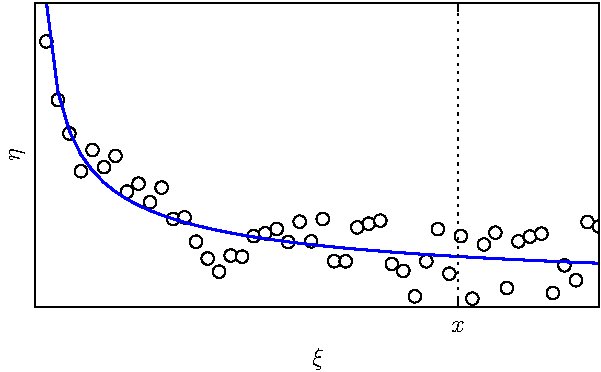
\includegraphics[width=\textwidth]{fig/covar-hyperb.pdf}
			\caption{Нелинейная зависимость}
      \end{figure}
  \end{minipage}
  \hspace{0.02\textwidth}
  \begin{minipage}{0.47\textwidth}
      \begin{figure}[H]
          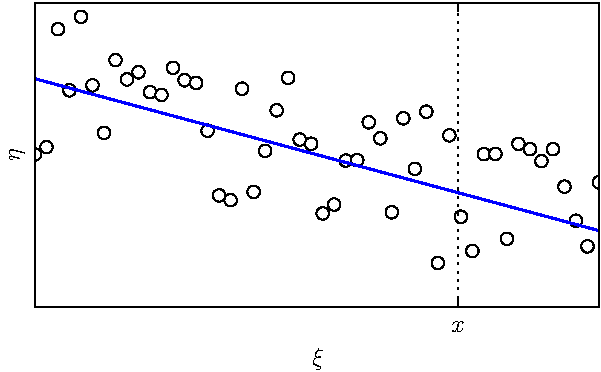
\includegraphics[width=\textwidth]{fig/covar-linear.pdf}
          \caption{Линейная зависимость}
      \end{figure}
  \end{minipage}
\end{minipage}
\begin{defn*}
Мера \emph{линейной} зависимости между случайным величинами $\xi$
и $\eta$ есть \emph{коэффициент корреляции Пирсона}
\[
\rho=\frac{\cov(\xi,\eta)}{\sqrt{\D\xi}\sqrt{\D\eta}}.
\]
\end{defn*}
\begin{rem*}
Про $\rho$ можно думать как про $\cos$ между векторами в соответствующем
пространстве.
\end{rem*}

\begin{rem*}[Важное]
\begin{eqnarray*}
\xi\indep\eta & \implies & \rho=0\\
\xi,\eta\sim\N(\mu,\sigma^{2}),\ \xi\indep\eta & \iff & \rho=0.
\end{eqnarray*}
\end{rem*}
\begin{prop*}
Для линейно зависимых данных, конечно, $\rho=1$.\end{prop*}
\begin{proof}
Пусть $\eta=a+b\xi$; тогда
\begin{eqnarray*}
\rho(\xi,\eta) & = & \frac{\cov(\xi,a+b\xi)}{\sqrt{\D\xi}\sqrt{\D(a+b\xi)}}=\frac{\E\xi(a+b\xi)-\E\xi\E(a+b\xi)}{\sqrt{\D\xi}\sqrt{\D b\xi}}=\frac{\E\xi a+b\E\xi^{2}-\E\xi\E a-\E\xi b\E\xi}{b\sqrt{\D\xi}\sqrt{\D\xi}}=\\
 & = & \frac{a\E\xi+b\E\xi^{2}-a\E\xi-b(\E\xi)^{2}}{b\D\xi}=\frac{b(\E\xi^{2}-(\E\xi)^{2})}{b\D\xi}=1.
\end{eqnarray*}

\end{proof}

\section{О соотношении $\rho$ и коэффициента линейной регрессии}

По (\ref{claim:linreg-coeffs}), если линейная регрессия уравнением
$y=kx+b$, то
\[
k=\rho\frac{\sigma_{\eta}}{\sigma_{\xi}}.
\]


В общем случае, по виду прямой линейной регрессии ничего нельзя сказать
о зависимости между случайными величинами. Так, если $\eta=a+b\xi$
есть линейная функция от $\xi$, то, по предыдущему, $\rho=1$ и
\[
k=1\cdot\frac{\sqrt{\D(a+b\xi)}}{\sqrt{\D\xi}}=b
\]
 и прямая может иметь произвольный, в зависимости от $b$, наклон.
\begin{rem*}
В то же время, поскольку для
\[
\begin{pmatrix}\xi\\
\eta
\end{pmatrix}\sim\N(\boldsymbol{\mu},\Sigma),\quad\Sigma=\begin{pmatrix}\sigma_{\xi}^{2} & \cov(\xi,\eta)\\
\cov(\xi,\eta) & \sigma_{\eta}^{2}
\end{pmatrix}
\]
справедливо, что
\[
k=\rho\frac{\sigma_{\eta}}{\sigma_{\xi}}=\frac{\cov(\xi,\eta)}{\sigma_{\xi}\sigma_{\eta}}\cdot\frac{\sigma_{\eta}}{\sigma_{\xi}}=\frac{1}{\sigma_{\xi}^{2}}\cov(\xi,\eta),
\]
 то $k=0\iff\cov(\xi,\eta)=0,$ а для стандартно нормальных данных
$k=\rho=\cov(\xi,\eta)$.
\end{rem*}

\section{Значимость коэффициента корреляции}
\begin{defn*}
Коэффициент корреляции \emph{значим}, если отвергается $H_{0}:\rho=0$.
\end{defn*}
Чаще, чем $H_{0}:\rho=\rho_{0}$, проверяют $H_{0}:\rho>\rho_{0}$.
Если $\rho_{0}=0,$ то $\left(\xi,\eta\right)^{\T}\sim\N(\boldsymbol{\mu},\boldsymbol{\Sigma})$
и, по ЦПТ, %
\begin{comment}
$\hat{\rho}\sim N$?
\end{comment}
\begin{comment}
По теореме Кохрана --- нетривиальный вывод
\end{comment}
{}
\[
T=\frac{\sqrt{n-2}\hat{\rho}_{n}}{\sqrt{1-\hat{\rho}_{n}^{2}}}\sim\t(n-2).
\]
Идеальное значение --- 0, два хвоста.

Если $\rho_{0}\neq0,$ то ЦПТ не работает, тогда распределение $\hat{\rho}$
неизвестно. Тогда применяется $z$-преобразование Фишера
\[
z=\frac{1}{2}\ln\frac{1+\rho}{1-\rho},\quad z_{0}=\frac{1}{2}\ln\frac{1+\rho_{0}}{1-\rho_{0}}.
\]
 Тогда ЦПТ работает и, если $\left(\xi,\eta\right)^{\T}\sim\N(\boldsymbol{\mu},\boldsymbol{\Sigma})$,
\[
T=\sqrt{n-3}(z-z_{0})\tod\N(0,1).
\]



\chapter{Метод наименьших квадратов (Ordinary Least Squares)}

Пусть $\eta,\xi\in L^{2}(\F,\P)$ пространству $\F$-измеримых по
мере $\P$ функций с конечным вторым моментом и скалярным произведением
$\left(\eta,\xi\right)=\E\eta\xi$, причем $\hat{\eta}\in K=\left\{ \phi(\xi)\right\} =\left\{ \hat{\eta}:\sigma(\phi(\xi))\text{-измерима}\right\} $.
По свойству УМО(\ref{prop:consistent_est}), вектор
\[
\hat{\eta}^{*}=\E\left\{ \eta\mid\phi(\xi)\right\}
\]
 будет ортогональной проекцией $\eta$ на $K$, т.е. $\left(\eta-\hat{\eta}^{*},\hat{\eta}\right)=0\ \forall\hat{\eta}\in K$.
Значит, он минимизирует квадрат нормы расстояния от $\eta$ до $K$:
\[
\hat{\eta}^{*}=\argmin_{\hat{\eta}\in K}\left\Vert \eta-\hat{\eta}\right\Vert ^{2}=\argmin_{\hat{\eta}\in K}\E\left(\eta-\hat{\eta}\right)^{2}=\E\left\{ \eta\mid\phi(\xi)\right\} .
\]
 $\hat{\eta}^{*}$ называется \emph{наилучшим среднеквадратичным приближением
в классе} $K$.


\chapter{Корреляционное отношение}

Если $K=\mathcal{L}=\left\{ a\xi+b\right\} $ --- линейное пространство,
то теорема Пифагора принимает вид
\[
\D\eta=\E\left(\eta-\E\eta\right)^{2}=\underbrace{\E\left(\hat{\eta}^{*}-\E\eta\right)^{2}}_{\text{объяснённая доля аппроксимации}}+\underbrace{\E\left(\eta-\hat{\eta}^{*}\right)^{2}}_{\text{ошибка аппроксимации}}.
\]
 Откуда можно записать меру аппроксимации
\[
\frac{\E(\hat{\eta}^{*}-\E\eta)^{2}}{\D\eta}=1-\frac{\E\left(\eta-\hat{\eta}^{*}\right)^{2}}{\D\eta}=1-\frac{\min_{\hat{\eta}\in\mathcal{L}}\E\left(\eta-\hat{\eta}\right)^{2}}{\D\eta}.
\]

\begin{defn*}
Полученная величина называется коэффициентом корреляции $\rho^{2}$:
\[
\rho^{2}:=1-\frac{\min_{\hat{\eta}\in\mathcal{L}}\E\left(\eta-\hat{\eta}\right)^{2}}{\D\eta}.
\]
 $\rho$ --- коэффициент корреляции Пирсона.
\end{defn*}

\begin{defn*}
\emph{Множественный коэффициент корреляции} есть полученная величина
для МНК с $K=\mathcal{M}=\left\{ \sum_{i=1}^{k}b_{i}\xi_{i}+b_{0}\right\} $.
\[
R^{2}(\eta,\xi_{1},\ldots,\xi_{k}):=1-\frac{\min_{\hat{\eta}\in\mathcal{M}}\E\left(\eta-\hat{\eta}\right)^{2}}{\D\eta}.
\]
\end{defn*}
\begin{rem*}
$R^{2}\geq\rho^{2}$; если же $R^{2}=\rho^{2}$, то $\xi_{1},\ldots,\xi_{k}$
все зависимы.\end{rem*}
\begin{defn*}
В общем случае, если $K=\left\{ \phi(\xi)\mbox{ измеримые}\right\} $,
то полученная величина называется \emph{корреляционным отношением}:

\[
r_{\eta\mid\xi}^{2}:=1-\frac{\min_{\hat{\eta}\in K}\E\left(\eta-\hat{\eta}\right)^{2}}{\D\eta}=\frac{\D\E(\eta\mid\xi)}{\D\eta}.
\]

\end{defn*}

\section{Свойства корреляционного отношения}
\begin{enumerate}
\item $r_{\eta\mid\xi}^{2}\in\left[0,1\right]$.
\item $\eta\indep\xi\implies r_{\eta\mid\xi}^{2}=0$.
\item $\eta=\phi(\xi)\iff r_{\eta\mid\xi}^{2}=1.$
\item Вообще говоря, $r_{\eta\mid\xi}^{2}\neq r_{\xi\mid\eta}^{2}$ . К
примеру, для любой не монотонной функции (так, чтобы не существовала
обратная).
\item $r_{\eta\mid\xi}^{2}\geq\rho^{2}(\eta,\xi)$ (потому что минимум по
всем функциям меньше, чем лишь по линейным, значит $1-\min$ больше).
\item $\left(\xi,\eta\right)^{\T}\sim\N(\boldsymbol{\mu},\boldsymbol{\Sigma})\implies r_{\eta\mid\xi}^{2}=\rho^{2}(\eta,\xi)$.
\end{enumerate}

\section{Выборочное корреляционное отношение}

По разложению дисперсии,

\[
\D\eta=\E(\eta-\E\eta)^{2}=\underbrace{\E(\E(\eta\mid\xi)-\E\eta)^{2}}_{\D\E(\eta\mid\xi)}+\E(\eta-\E(\eta\mid\xi))^{2}.
\]
 Перейдем на выборочный язык. Пусть дана выборка
\[
\begin{pmatrix}x_{1}\\
y_{1}
\end{pmatrix},\ldots,\begin{pmatrix}x_{n}\\
y_{n}
\end{pmatrix}.
\]
 Сгруппируем её:

\begin{center}
\begin{tabular}{c|ccc}
$x_{1}^{*}$ & $y_{11}$ & $\dots$ & $y_{1n_{1}}$\tabularnewline
$\vdots$ & $\vdots$ & $\ddots$ & $\vdots$\tabularnewline
$x_{k}^{*}$ & $y_{k1}$ & $\dots$ & $y_{kn_{k}}$\tabularnewline
\end{tabular}
\par\end{center}

Пусть $\xi$ --- дискретная случайная величина со значениями $\left(x_{1}^{*},\ldots,x_{k}^{*}\right)$.
Тогда, учитывая
\[
\bar{y}_{i}=\bar{y}_{i\cdot}=\frac{1}{n_{i}}\sum_{j=1}^{n_{1}}y_{ij}=\hat{\E}(\eta\mid\xi=x_{i}^{*}),
\]
на выборочном языке получаем (домножив на $n$):
\begin{eqnarray*}
\underbrace{\sum_{i=1}^{k}\sum_{j=1}^{n_{i}}(y_{ij}-\bar{y})^{2}}_{\text{total sum of squares}} & = & \underbrace{\sum_{i=1}^{k}n_{i}\left(\bar{y}_{i}-\bar{y}\right)^{2}}_{\text{межгрупповой разброс}}+\underbrace{\sum_{i=1}^{k}\sum_{j=1}^{n_{i}}(y_{ij}-\bar{y}_{i})^{2}}_{\text{внутригрупповой разброс}}\\
ns_{y}^{2} & = & ns_{y\mid x}^{2}+\sum_{i=1}^{k}\sum_{j=1}^{n_{i}}(y_{ij}-\bar{y}_{i})^{2}.
\end{eqnarray*}
 Отсюда, так как, $r_{\eta\mid\xi}^{2}=\D\E(\eta\mid\xi)/\D\eta$,

\[
\hat{r}_{\eta\vert\xi}^{2}=\hat{r}_{y\vert x}^{2}=\frac{s_{y\vert x}^{2}}{s_{y}^{2}}.
\]



\chapter{Частная корреляция}
\begin{defn*}
Частная корреляция случайных величин $\eta_{1},\eta_{2}$ относительно
$\left\{ \xi_{1},\ldots,\xi_{k}\right\} $ есть
\[
\rho\left(\eta_{1},\eta_{2}\mid\left\{ \xi_{1},\ldots,\xi_{k}\right\} \right):=\rho\left(\eta_{1}-\hat{\eta}_{1}^{*},\eta_{2}-\hat{\eta}_{2}^{*}\right),\quad\text{где }\hat{\eta}_{i}^{*}=\argmin_{\hat{\eta}_{i}\in\left\{ \sum_{i=1}^{k}b_{i}\xi_{i}+b_{0}\right\} }\E\left(\eta_{i}-\hat{\eta}_{i}\right)^{2}.
\]

\end{defn*}
\begin{comment}
@xio: $\E(\eta\mid\xi_{1},\ldots,\xi_{k}):=$ наилучшее функциональное
приближение --- регрессия; наилучшее приближение по МНК --- линейная
регрессия.
\end{comment}


Если регрессия линейна, то
\[
\rho(\eta_{1},\eta_{2}\mid\xi_{1},\ldots,\xi_{k})=\rho(\eta_{1}-\E\left\{ \eta_{1}\mid\xi_{1},\ldots,\xi_{k}\right\} ,\eta_{2}-\E\left\{ \eta_{2}\mid\xi_{1},\ldots,\xi_{k}\right\} ).
\]

\begin{rem*}[Важное]
Пусть в эксперименте подсчитан ненулевой $\rho$. Это может означать,
что один из факторов является причиной, а другой следствием; чтобы
установить, что есть что, проводят эксперимент и смотрят, какой фактор
в реальности влияет на какой. Это может также означать, что влияет
сторонний фактор. Чтобы его исключить, считают частную корреляцию.\end{rem*}
\begin{example*}
Возможна ситуация, когда $\rho(\eta_{1},\eta_{2})\neq0$, но $\rho(\eta_{1},\eta_{2}\mid\xi)=0$.
Частная корреляция есть, по сути, корреляция на центрированных данных.

\begin{minipage}{\textwidth}
  \centering
  \begin{minipage}{0.47\textwidth}
      \begin{figure}[H]
          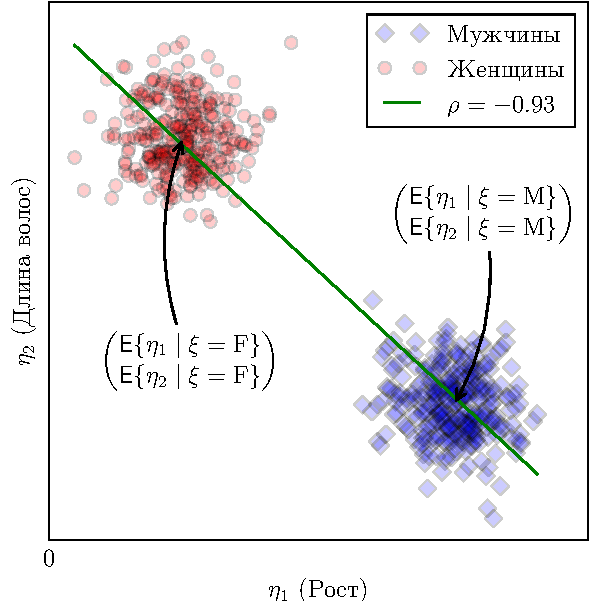
\includegraphics[width=\textwidth]{fig/part_corr-mf.pdf}
			\caption{Исходные данные (бимодальность)}
      \end{figure}
  \end{minipage}
  \hspace{0.02\textwidth}
  \begin{minipage}{0.47\textwidth}
      \begin{figure}[H]
          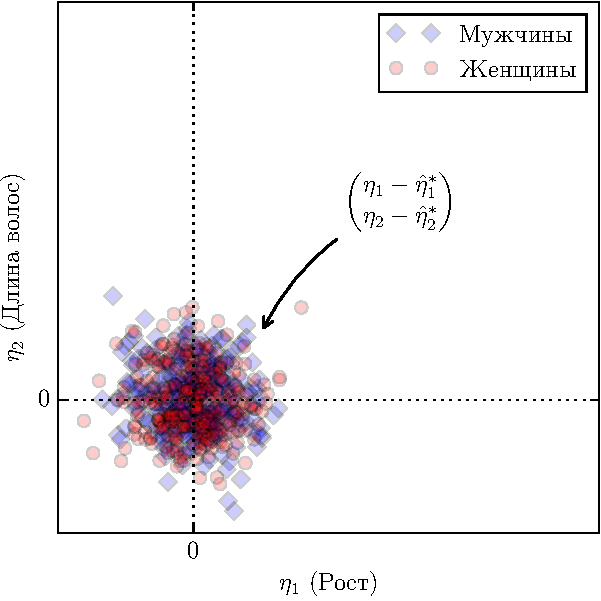
\includegraphics[width=\textwidth]{fig/part_corr_centered-mf.pdf}
          \caption{Центрированные данные}
      \end{figure}
  \end{minipage}
\end{minipage}
\end{example*}

\begin{example*}
Возможна и ситуация как на (\ref{fig:part_covar-bivar_gauss}), где
определенно $\rho(\eta_{1},\eta_{2})>0$, но $\rho(\eta_{1},\eta_{2}\mid\xi)<0$.

\begin{center}
\begin{figure}[H]
\begin{centering}
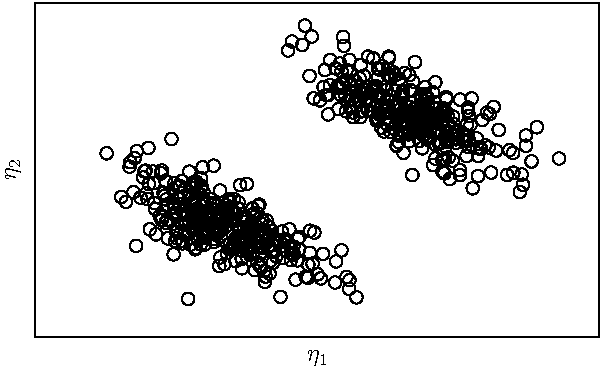
\includegraphics[width=0.6\textwidth]{fig/part_corr-bivar_gauss}
\par\end{centering}

\caption{\label{fig:part_covar-bivar_gauss}$\rho(\eta_{1},\eta_{2})>0$, но
$\rho(\eta_{1},\eta_{2}\mid\xi)<0$}
\end{figure}

\par\end{center}

\end{example*}
\begin{rem*}
По аналогии с предыдущим примером, если $\left|\im\xi\right|\to\infty$,
то графики $\left(\eta_{1},\eta_{2}\right)$ при фиксированном $\xi$
образуют эллипсоид (в этом случае с положительной корреляцией).
\end{rem*}
\begin{comment}
Data analysis case

CARDATA

Почему цена не зависит от других характеристик
\begin{enumerate}
\item Смотрим matrixplot
\item Логарифмируем данные; тогда

\begin{enumerate}
\item Длинные хвосты укорачиваются
\item Надежнее можно классифицировать точки как аутлаеров
\item Если признак lognormal, то log(lognormal) = normal и нелинейные зависимости
становятся линейными.
\item Некоторые критерии становятся точными (?)
\end{enumerate}
\item При помощи brushing tool (или select cases (кажется)) убираем аутлаеров
в логданных.
\item Ищем неоднородности в данных. По качественному признаку (origin) нельзя
делать частную регрессию, поэтому строим clustered correlation plot,
на котором смотрим зависимость мощности от логцены по origin. Видим,
что американские данные отличаются от европейских + японских. Можем
построить correlation matrix по group by origin.
\item Смотрим clustered correlation plot по году и видим, что год размывает
отчетливую тенденцию. Частную регрессию \emph{можно} делать с контролем
по дискретному количественному признаку (год).
\item In the end, делаем частную регрессию с контролем по году и group by
origin. \end{enumerate}
\end{comment}


\begin{comment}
Преобразования данных:
\begin{itemize}
\item $\log(x+1)$
\item $1/(x+1)$ стабилизирует дисперсию
\item $\log\left(\frac{x}{1-x}\right)$ (logit) или $\arcsin\sqrt{x}$:
выпрямляет сигмоиды\end{itemize}
\end{comment}


\begin{comment}
Нормализация данных: scale(c(1, 3, 5))
\end{comment}



\chapter{Зависимость между порядковыми признаками}

Пусть на выборке
\[
\begin{pmatrix}\xi\\
\eta
\end{pmatrix}\sim\begin{pmatrix}x_{1}\\
y_{1}
\end{pmatrix},\ldots,\begin{pmatrix}x_{n}\\
y_{n}
\end{pmatrix}
\]
 задан только порядок. Тогда можем считать только эмпирическую функцию
распределения.

Следующие коэффициенты основаны на рангах. Ранговые характеристики
хорошо работают на выборках \emph{без повторений} (чтобы, к примеру,
не возникало дробных рангов).


\section{Ранговый коэффициент Спирмана}
\begin{defn*}
\emph{Ранговый коэффициент Спирмана} есть
\[
\rho_{S}=\rho(\cdf_{\xi}(\xi),\cdf_{\eta}(\eta)).
\]
\begin{comment}
@xio: как это понимать?
\end{comment}
\end{defn*}
\begin{rem*}
$\cdf_{\xi}(\xi)\sim\U(0,1)$, потому что $\P(\cdf_{\xi}(\xi)<x)=\P(\xi<\cdf_{\xi}^{-1}(x))=\cdf_{\xi}(\cdf_{\xi}^{-1}(x))=x$.
\end{rem*}

\begin{defn*}
\emph{Ранг} элемента из выборки есть его порядковый номер в упорядоченной
выборке:
\[
\rk x_{(i)}=i.
\]
\end{defn*}
\begin{notation*}
$\rk x_{(i)}=:R_{i}$, $\rk y_{(i)}=:T_{i}$.
\end{notation*}
Можем ввести эмпирическое распределение
\[
\cdf_{\xi_{n}}(x_{i})=\frac{\rk x_{i}}{n},\quad\cdf_{\eta_{n}}(y_{i})=\frac{\rk y_{i}}{n}=\frac{T_{i}}{n}.
\]
 %
\begin{comment}
\[
\begin{pmatrix}\begin{pmatrix}R_{1}/n\\
T_{1}/n
\end{pmatrix} & \cdots & \begin{pmatrix}R_{n}/n\\
T_{n}/n
\end{pmatrix}\\
1/n & \cdots & 1/n
\end{pmatrix}.
\]
\end{comment}
Тогда будет справедливо следующее
\begin{defn*}
\emph{Выборочный коэффициент Спирмана} определяется как выборочный
коэффициент корреляции Пирсона $\hat{\rho}$, но с заменой значений
на ранги:
\[
\hat{\rho}_{S}\begin{pmatrix}\xi_{n}\\
\eta_{n}
\end{pmatrix}=\rho\begin{pmatrix}R_{n}\\
T_{n}
\end{pmatrix}=\frac{1/n\cdot\sum_{i=1}^{n}R_{i}T_{i}-\bar{R}\bar{T}}{\sqrt{1/n\cdot\sum_{i=1}^{n}\left(R_{i}-\bar{R}\right)^{2}}\sqrt{1/n\cdot\sum_{i=1}^{n}\left(T_{i}-\bar{T}\right)^{2}}}.
\]


Если нет повторяющихся наблюдений, то знаменатель будет одним и тем
же у всех выборок объема $n$, значит его можно посчитать заранее.
В этом (и только этом) случае, справедлива более простая формула:
\[
\hat{\rho}_{S}=1-\frac{6\sum_{i=1}^{n}(R_{i}-T_{i})^{2}}{n^{3}-n}.
\]
\end{defn*}
\begin{rem*}
Из последней формулы хорошо видно, что если $x_{i},y_{i}$ все идут
в одном порядке, то $R_{i}-T_{i}=0\ \forall i$ и $\hat{\rho}_{S}=1$.
\end{rem*}

\begin{rem*}
$\rho_{S}$ для \emph{количественных} признаков есть мера монотонной
зависимости:
\[
\rho_{S}=1\iff(x_{i}>x_{i+1}\implies y_{i}>y_{i+1}\ \forall i)
\]
(даже если зависимость нелинейная и $\rho\neq1$). Иными словами,
$\rho_{S}>0$, если $y$ имеет тенденцию к возрастанию с возрастанием
$x$ (и $\rho_{S}<0$ иначе). Чем большое $\rho_{S}$, тем более явно
выражена зависимость $y$ от $x$ в виде некоторой монотонной функции.
\end{rem*}

\subsection{Согласованость $\rho$ и $\rho_{S}$}

$\rho_{S}$ не согласована с $\rho$ в том же смысле, что $\rho$
и $r_{\xi\mid\eta}$. %
\begin{comment}
@xio: FIXME: т.е.?
\end{comment}

\begin{claim*}
Если данные нормальные то справедлива формула
\[
\rho=2\sin\left(\frac{\pi}{6}\rho_{S}\right).
\]
 Значит, можем сравнить критерии между собой.\end{claim*}
\begin{itemize}
\item С точностью до погрешности, по значению, $\hat{\rho}$ и $\hat{\rho}_{S}$
--- это одно и то же (см. \ref{fig:rho-rho_S})


\begin{figure}[H]
\begin{centering}
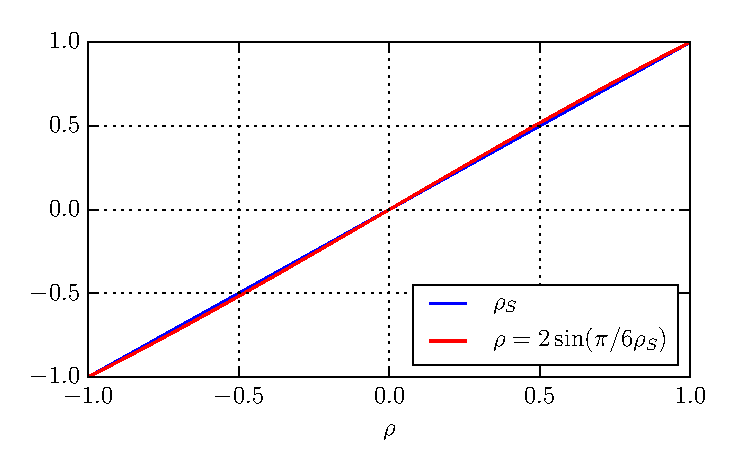
\includegraphics[width=0.6\textwidth]{fig/rho-rho_S}
\par\end{centering}

\captionbelow{\label{fig:rho-rho_S}$\hat{\rho}\approx\hat{\rho}_{S}$}
\end{figure}


\item Обычный критерий оценки --- выборочную дисперсию --- посчитать сложно.
Тем не менее, можем заметить, что $\hat{\rho}_{S}$ более устойчив
к аутлаерам (см. \ref{fig:rho-outlier}). Всегда можно добавить аутлаер
такой, что $\hat{\rho}=0$; $\hat{\rho}_{S}$ же поменяется не сильно.
Поэтому для нормальных данных, $\rho_{S}$ --- это оценка, что нет
аутлаеров.


\begin{figure}[H]
\begin{centering}
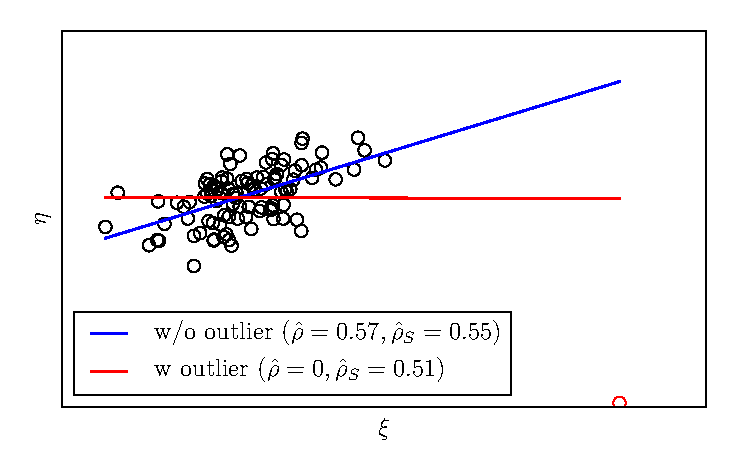
\includegraphics[width=0.6\textwidth]{fig/rho_outlier}
\par\end{centering}

\captionbelow{$\hat{\rho}$ до и после добавления аутлаера\label{fig:rho-outlier}}
\end{figure}


\item Монотонным преобразованием можем всегда сделать так, чтобы $\rho$
изменился (например, возведя в квадрат); при монотонном преобразовании,
однако, не меняется $\rho_{S}$ (см. \ref{fig:rho-monotone}). Значит,
чтобы узнать $\rho$ исходных (нормальных) данных, можно не выполнять
обратного преобразования, а сразу посчитать $\rho_{S}$.


\begin{figure}[H]
\begin{centering}
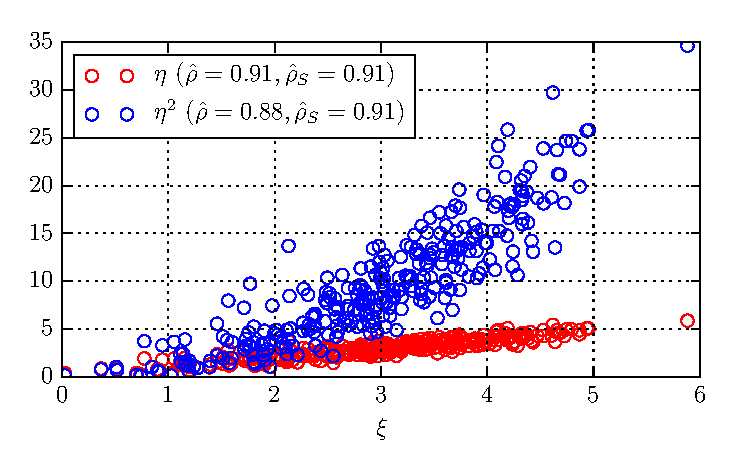
\includegraphics[width=0.6\textwidth]{fig/rho_monotone}
\par\end{centering}

\captionbelow{Монотонное преобразование нормальных данных\label{fig:rho-monotone}}
\end{figure}


\end{itemize}

\section{Ранговый коэффициент Кэндалла $\tau(\xi,\eta)$}
\begin{defn*}
Пусть $\left(\xi_{1},\eta_{1}\right)^{\T}\indep\left(\xi_{2},\eta_{2}\right)^{\T}\sim\Pcal_{\xi,\eta}\sim\left(\xi,\eta\right)^{\T}$;
тогда \emph{ранговым коэффициентом Кэндалла} называется
\[
\tau(\xi,\eta)=\rho(\sign(\xi_{2}-\xi_{1}),\sign(\eta_{2}-\eta_{1}))=\P((\xi_{2}-\xi_{1})(\eta_{2}-\eta_{1})>0)-\P((\xi_{2}-\xi_{1})(\eta_{2}-\eta_{1})<0).
\]


На выборочном языке, пусть дана выборка $(x_{1},y_{1}),\ldots,(x_{n},y_{n})$;
тогда
\[
\tau=\frac{\#(\text{одинаково упорядоченных пар})-\#(\text{по-разному упорядоченных пар})}{\#(\text{комбинаций пар})},
\]
 где пара $(x_{i},y_{i}),(x_{j},y_{j})$ считается одинаково упорядоченной,
если $\sign(x_{i}-x_{j})=\sign(y_{i}-y_{j})$, а $\#(\text{комбинаций пар})=C_{n}^{2}=n(n-1)/2$.\end{defn*}
\begin{claim*}
Если $(\xi,\eta)^{\T}\sim\N(\boldsymbol{\mu},\Sigma)$, то справедлива
формула
\[
\rho=\sin\left(\frac{\pi}{2}\tau\right).
\]

\end{claim*}
Из утверждения следует, что $\tau$ все время меньше $\rho$ и $\rho_{S}$
(по модулю).
\begin{figure}[H]
\begin{centering}
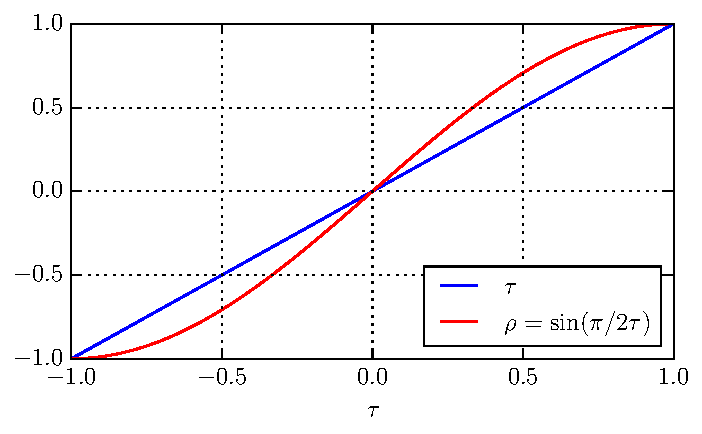
\includegraphics[width=0.6\textwidth]{fig/rho-tau}
\par\end{centering}

\captionbelow{$\rho$ и $\tau$}
\end{figure}

\begin{example*}[Проверка ряда на тренд]
Пусть $\xi$ --- номера точек, а $\eta$ --- значения ряда. Тогда
$H_{0}:\tau_{0}=0$ и если $H_{0}$ отвергается, то тренд присутствует.
\begin{comment}
@xio: FIXME: прояснить!
\end{comment}
\begin{comment}
Т.е. если тренд есть, то $x_{i}>x_{i+1}\implies y_{i}>y_{i+1}$ с
большой вероятностью.
\end{comment}

\end{example*}
\begin{comment}
Еще одна мера порядковых зависимостей:
\[
\gamma=\frac{\tau}{1-\P(\xi=\eta)}.
\]
\end{comment}



\chapter{Корреляционные матрицы}

Если признаков много, то их наглядно характеризуют корреляционные
матрицы. Улучшить наглядность можно переупорядочив признаки так, чтобы
на диагонали матрицы стояли блоки корреляций признаков из <<корреляционных
плеяд>>.
\begin{defn*}
Пусть $\rho_{0}$; корреляционная плеяда есть множество признаков,
таких, что их попарная корреляция больше $\rho_{0}$.
\end{defn*}
Можно выделить и несколько уровней $\rho_{i}:\rho_{0}<\rho_{1}<\dots$.
Тогда сначала следует составить плеяду по $\rho_{0}$, затем внутри
полученного по $\rho_{1}$ и т.д.


\part{Дисперсионный анализ}


\chapter{Однофакторный дисперсионный анализ (One-way ANOVA\protect\footnote{ANalysis Of VAriation})}

Задача может быть поставлена двумя эквивалентными образами:
\begin{enumerate}
\item Пусть $\eta_{i}\sim\Pcal_{i},\ i\in1:k$. Проверить гипотезу, что
все распределения равны:
\[
H_{0}:\Pcal_{1}=\dots=\Pcal_{k}.
\]

\item Пусть дан двумерный вектор $\begin{pmatrix}\xi & \eta\end{pmatrix}^{\T}$,
причем $\xi$ (<<фактор>>) принимает $k$ значений $A_{1},\ldots,A_{k}$.
Рассмотрим $\eta_{i}\sim\Pcal_{i}=\Pcal_{\eta\mid\xi=A_{i}}$. Проверить
гипотезу
\[
H_{0}:\Pcal_{\eta\mid\xi=A_{1}}=\dots=\Pcal_{\eta\mid\xi=A_{k}}.
\]

\end{enumerate}
Пусть теперь $\eta_{i}\sim\N(\mu_{i},\sigma^{2})$. Разумеется,
\begin{multline*}
H_{0}:\mu_{1}=\dots=\mu_{k}\iff H_{0}:\E\eta_{1}=\dots=\E\eta_{k}\\
\iff H_{0}:\E(\eta\mid\xi=A_{1})=\dots=\E(\eta\mid\xi=A_{k})\iff H_{0}:\D\E(\eta\mid\xi)=0.
\end{multline*}


Для построения критерия, вспомним разложение дисперсии на выборочном
языке:
\[
\underbrace{\sum_{i=1}^{k}\sum_{j=1}^{n_{i}}(y_{ij}-\bar{y})^{2}}_{Q=\hat{\D}\eta}=\underbrace{\sum_{i=1}^{k}n_{i}\left(\bar{y}_{i}-\bar{y}\right)^{2}}_{Q_{1}=\hat{\D}\E(\eta\mid\xi)}+\underbrace{\sum_{i=1}^{k}\sum_{j=1}^{n_{i}}(y_{ij}-\bar{y}_{i})^{2}}_{Q_{2}},
\]
 откуда в качестве критерия (следуя гипотезе) выберем $Q_{1}$ с идеальным
значением $0$. Однако $Q_{1}$ полезно отнормировать по $Q_{2}$
для учета различных внутригрупповых разбросов. Чтобы получить статистику
с известным распределением, вспомним, что по теореме Cochran, $Q_{1}\indep Q_{2},$
\begin{comment}
Почему?
\end{comment}
\[
\frac{Q}{\sigma^{2}}\sim\chi^{2}(n-1),\quad\frac{Q_{1}}{\sigma^{2}}\sim\chi^{2}(k-1),\quad\frac{Q_{2}}{\sigma^{2}}\sim\chi^{2}(n-k)
\]
{} и
\[
t=\frac{Q_{1}/(k-1)}{Q_{2}/(n-k)}\sim\mathrm{F}((k-1),(n-k)).
\]

\begin{rem*}
Это обобщение статистики для проверки гипотезы о равенстве математических
ожиданий независимых двумерных выборок с равными дисперсиями (с $k=2$,
то есть):
\[
t=\frac{\bar{x}-\bar{y}}{\tilde{s}_{1,2}\sqrt{1/n_{1}+1/n_{2}}}
\]
 с $\tilde{s}_{1,2}^{2}=Q_{2}/(n-2)$. Дело в том, что статистики
распределены одинаковы --- по определению,
\[
t^{2}(n-2)=\mathrm{F}(1,n-2).
\]

\end{rem*}
Чтобы воспользоваться полученным критерием, должно убедиться, что
дисперсии одинаковые. Как и в случае $k=2$, это можно проверить по
тесту Левена, только многомерному, т.е. проверить равенство математических
ожиданий $\E\left|\xi-\E\xi_{i}\right|\ \forall i\in1:k$, $\left|y_{ij}-\bar{y}_{i}\right|$
--- опять же, через саму ANOVA.
\begin{rem*}
Если условия нормальности нарушаются, то критерий становится асимптотическим.
Тогда вместо $\mathrm{F}$ следует использовать $\chi^{2}$, так как
$\mathrm{F}(k,m)/m\xrightarrow[m\to\infty]{}\chi^{2}(k)$.\end{rem*}
\begin{example*}
Пусть дана выборка вида $\left\{ \left(\xi=\text{пол},\eta=\text{вес}\right)\right\} $.
Выдвинем $H_{0}:$ вес не зависит от пола. Очевидно, что $\xi$ ---
категориальная случайная величина, а $\eta$ --- количественная. Значения
$\xi$ разобьют всю выборку на две (?) группы. Тогда проверка гипотезы
сведется к проверке равенства распределений в двух группах, $\Pcal_{\eta\mid\xi=s_{1}}=\Pcal_{\eta\mid\xi=s_{2}}.$
В предположении, что $\left(\eta\mid\xi=s_{i}\right)\sim\N(\mu_{i},\sigma^{2})$,
равенство распределений будет следовать из равенства математических
ожиданий.
\end{example*}

\chapter{Множественные сравнения}
\begin{example*}
Проблема множественных сравнений возникает, например, в следующих
ситуациях.
\begin{itemize}
\item Пусть одна группа испытуемых принимает лекарство, а вторая нет. По
завершению эксперимента две группы сравниваются по $m$ показателям.
Однако чем больше показателей сравнивается, тем больше вероятность
того, что \emph{хотя бы по одному} показателю будет совпадение (в
силу случайности).
\item Испытывают $m=100$ монет на честность сериями по $n=10$ бросков:\\
 $\{(\xi_{1}^{(1)},\ldots,\xi_{10}^{(1)}),\ldots,(\xi_{1}^{(100)},\ldots,\xi_{10}^{(100)})\}$,
иными словами $\left\{ \eta^{(1)},\ldots,\eta^{(100)}\right\} ,$
где $\eta^{(i)}\sim\Bin(10,p)$. Проверить $m$ гипотез $H_{0}^{(i)}:\eta^{(i)}\sim\Bin(10,1/2)$,
$i\in1:m$. Зафиксируем $\a=0.05$. Тогда, учитывая $\pmf_{\Bin(10,1/2)}(k)=C_{10}^{k}2^{-10}$,
$\P_{H_{0}^{(i)}}(\eta^{(i)}\geq9)=10\cdot2^{-10}+1\cdot2^{-10}\approx0.0107,$
однако уже $\P_{H_{0}^{(i)}}(\eta^{(i)}\geq8)\approx0.0546$. Так
что критерием наибольшей мощности будет $\eta^{(i)}\geq9$:
\[
\a_{1}=\P_{H_{0}^{(i)}}(H_{0}^{(i)}\text{ отв})=\P_{H_{0}^{(i)}}(\eta^{(i)}\geq9)\approx0.0107\leq0.05.
\]
 Но использование того же критерия для множественных сравнений сильно
завышает $\a_{\I}$:%
\begin{comment}
FIXME: это делает критерий множественных сравнений радикальным? Дописать
\end{comment}
{}
\begin{eqnarray*}
\P\left(\bigvee_{i=1}^{100}H_{0}^{(i)}\text{ отв}\right) & = & 1-\P\left(\bigwedge_{i=1}^{100}H_{0}^{(i)}\text{ не отв}\right)=1-\left(1-\P(H_{0}^{(i)}\text{ отв})\right)^{100}\\
 & = & 1-(1-0.0107)^{100}\approx0.6589.
\end{eqnarray*}

\end{itemize}
\end{example*}
Пусть проверяются гипотезы $H_{0}^{(1)},\ldots,H_{0}^{(m)}$. Возможны
такие ситуации:

\begin{center}
\begin{tabular}{ccc}
\toprule
 & Retain $H_{0}$ (отличие от $H_{0}$ не значимо) & Reject $H_{0}$ (отличие от $H_{0}$ значимо)\tabularnewline
\midrule
True $H_{0}$ & \# True Negative & \# False Positive (False Discovery)\tabularnewline
\midrule
False $H_{0}$ & \# False Negative & \# True Positive (True Discovery)\tabularnewline
\bottomrule
\end{tabular}
\par\end{center}

Используя обозначения таблички,
\[
\a_{\I}\approx\frac{\mathrm{FP}}{\mathrm{TN+FP}},\qquad\a_{\II}\approx\frac{\mathrm{FN}}{\mathrm{FN+TP}}.
\]

\begin{defn*}
Family-wise error rate (FWER):
\[
\mathrm{FWER}=\P(\text{хотя бы один раз отвергнута верная гипотеза})=\P\left(\bigvee_{i=1}^{m}H_{0}^{(i)}\text{ отв}\right).
\]
 Иными словами, $\FWER$ --- это ошибка первого рода для всей совокупности
экспериментов.
\end{defn*}
Требуется контролировать $\FWER$ на предзаданном уровне $\a$, т.е.
чтобы $\FWER\sim\a,$ где $\sim\in\left\{ =,\leq,\to\right\} $. В
\emph{слабом} смысле это осуществляется, если $\FWER\sim\a$ только
если \emph{все} $H_{0}^{(i)},\ i\in1:m$ верны. В \emph{сильном} смысле
контроль $\FWER$ на уровне $\a$ гарантируется для \emph{любой} конфигурации
верных и не верных $H_{0}^{(j)}$.
\begin{defn*}
Пусть $T_{0}:=\left\{ i:H^{(i)}\text{ верна}\right\} .$ Тогда
\[
\weak\,\FWER_{T}=\P(\text{хотя бы один раз отвергнута верная гипотеза, если верны }H^{(i)},\ i\in T)
\]
 т.е. если $T_{0}=T$.
\end{defn*}

\begin{defn*}
\[
\strong\,\FWER=\max_{T:T\subset\left\{ 1,\ldots,m\right\} }\weak\,\FWER_{T}.
\]
\end{defn*}
\begin{notation*}
$\FWER_{T}:=\weak\,\FWER_{T}.$
\end{notation*}
Это осуществляется двумя процедурами:
\begin{itemize}
\item Single
\item Stepdown
\end{itemize}

\section{Single}

Каждая $H^{(i)}$ проверяется отдельно с уровнем значимости $\a_{1}$.
Задача сводится к тому, чтобы найти такое $\a_{1}$, что $\FWER\leq\a$
для какого-то нужного предзаданного $\a$. Пусть $T=1:m$, т.е. будто
все тесты верны; тогда
\[
\FWER_{\left\{ 1,\ldots,m\right\} }=\P\left(\bigvee_{i=1}^{m}H_{0}^{(i)}\text{ отв}\right)\leq\sum_{i=1}^{m}\P(H^{(i)}\text{ отв})=m\a_{1}=\a\implies\a_{1}:=\frac{\a}{m}.
\]

\begin{rem*}
Из-за неравенства тест консервативный, т.е. $\FWER\ll\a$. Значит
не максимально мощный.
\end{rem*}
\begin{comment}
FixME: почему?
\end{comment}
\begin{eqnarray*}
\strong\,\FWER & = & \max_{T\subset\left\{ 1,\ldots,m\right\} }\P(H^{(i)}\text{ отвергается},\ i\not\in T)\\
 & \leq & \sum_{i\not\in T}\P(H^{(i)}\text{ отвергается})=\left|\left\{ i:i\not\in T\right\} \right|\a_{1}=\a.
\end{eqnarray*}

\begin{cor*}
$\FWER$ всегда хуже $\strong\,\FWER.$%
\begin{comment}
FixME: почему?
\end{comment}
\end{cor*}
\begin{defn*}
Поправка Бонферрони
\[
\a_{1}=\frac{\a}{m}.
\]

\end{defn*}
Тест нужно проверять не с $\a_{1}$, а с $\a/m$. Так критерий будет
консервативным (иначе --- радикальным, что хуже).
\begin{defn*}
Поправка Бонферрони для $\pv$:
\[
\pv<\frac{\a}{m}\implies\text{отвергаем}\iff mp<\a\implies\text{отвергаем}.
\]

\end{defn*}

\section{Stepdown (Holm's algorithm)}

Для увеличения мощности применяется <<Holm's algorithm>>:
\begin{enumerate}
\item считаются все $\pv$ $p_{1},\ldots,p_{m}$,
\item упорядочиваются: $p_{(1)}\leq\ldots\leq p_{(m)}.$
\item если $mp_{(1)}<\a$ то гипотеза отвергается, иначе и все последующие
не отвергаются
\item в общем, если
\[
p_{(j)}<\frac{\a}{m-j+1}
\]
 то гипотеза отвергается, иначе и все последующие не отвергаются.\end{enumerate}
\begin{rem*}
Сей тест более мощный, потому что не всегда происходит умножение на
$m$.
\end{rem*}

\begin{rem*}
Процедуру сложно повторить, потому что при упорядочивании гипотезы
могут перемешиваться.\end{rem*}
\begin{prop*}
$\FWER\leq\a$.\end{prop*}
\begin{proof}
Упорядочим $\pv$: $p_{(1)}\leq\dots\leq p_{(j)}\leq\ldots\leq p_{(m)}.$
Пусть $I=\left\{ i:H_{0}^{(i)}\text{ верна}\right\} $, $m_{0}=\left|I\right|$
--- количество верных гипотез, $j=\min_{k\in I}$. $m_{0}$ должно
<<поместиться до конца>>:
\[
j\leq m-m_{0}+1\implies\frac{\a}{m-j+1}\leq\frac{\a}{m_{0}}.
\]
 Значит %
\begin{comment}
FIXME: почему?
\end{comment}
{}
\begin{eqnarray*}
\FWER_{I} & \leq & \P\left(p_{(j)}<\frac{\a}{m-j+1}\right)\leq\P\left(p_{(j)}<\frac{\a}{m_{0}}\right)\leq\P\left(\min_{i\in I}p_{i}<\frac{\a}{m_{0}}\right)\\
 & = & \P\left(\bigvee_{i\in I}p_{i}<\frac{\a}{m_{0}}\right)\leq\sum_{i\in I}\P\left(p_{i}<\frac{\a}{m_{0}}\right)=m_{0}\frac{\a}{m_{0}}=\a
\end{eqnarray*}

\end{proof}

\subsection{Частный случай}

Если все гипотезы и критерии независимы, то возможно точно посчитать
$\FWER$:
\begin{eqnarray*}
\FWER_{\left\{ 1,\ldots,m\right\} } & = & \P\left(\bigvee_{i=1}^{m}H_{0}^{(i)}\text{ отв}\right)=1-\P\left(\bigwedge_{i=1}^{m}H_{0}^{(i)}\text{ не отв}\right)\\
 & = & 1-(1-\a_{1})^{m}=\a\implies\a_{1}=1-\sqrt[m]{1-\a}
\end{eqnarray*}

\begin{defn*}
\emph{Поправка Šidák}:
\[
\a_{1}=1-\sqrt[m]{1-\a}.
\]

\end{defn*}

\chapter{ANOVA Post-Hoc Comparison}

В случае отвержения гипотезы ANOVA, можно провести дополнительное
выборочное тестирование выделенных групп.


\section{Least Significant Difference (LSD)}

LSD test --- это просто попарный $t$-test:
\[
t=\frac{\bar{\mathbf{y}}_{i}-\bar{\mathbf{y}}_{j}}{\tilde{s}_{1,\ldots,k}\sqrt{1/n_{i}+1/n_{j}}}\sim\t(n-k),
\]
 где $\tilde{s}_{1,\ldots,k}$ --- это pooled по $k$ группам standard
deviation.
\begin{rem*}
Его стоит применять после множественного сравнения лишь к тем группам,
важность которых была зафиксирована экспериментатором до проведения
множественного сравнения.
\end{rem*}

\begin{rem*}
Критерий радикален. Значит, если он не нашел разницу, то и другие
критерии тоже не найдут.
\end{rem*}

\begin{rem*}
Если групп немного, то можно применить поправку Бонферрони.
\end{rem*}

\section{Распределение размаха}

Сопоставим $\xi_{1},\ldots,\xi_{n}$ $\iid$ с $\cdf_{\xi_{i}}(x)=F(x)$
вариационный ряд $\xi_{(1)},\ldots,\xi_{(n)}$.
\begin{defn*}
\emph{Размах} есть случайная величина
\[
w_{n}=\xi_{(n)}-\xi_{(1)}
\]
 с функцией распределения
\[
\P(w_{n}<w)=n\int_{\RR}(F(x+w)-F(x))^{n-1}\d F(x)
\]
 ($w_{n}<w\implies w_{i}<w$, $\P(w_{i}<w)=F(x+w)-F(x)$ --- $n-1$
штук таких, плюс перебор разных минимумов по $1:n$).\end{defn*}
\begin{rem*}
В частном случае $F(x)=\cdf_{\N(0,\sigma^{2})}(x)$, $\Phi(x)=\cdf_{\N(0,1)}(x)$
рассматривается \emph{стандартизированный размах}
\[
\P\left(\frac{w_{n}}{\sigma}<w\right)=n\int_{\RR}(\Phi(x+w)-\Phi(x))^{n-1}\d\Phi(x).
\]
 Если $\sigma$ неизвестна, то с подставленной оценкой $w/\tilde{s}$
называется стьюдентизированным размахом.\end{rem*}
\begin{claim*}
\label{claim:studentized_range}Пусть $\ell$ --- некий параметр и
--- $\eta^{2}$ такая, что $\ell\eta^{2}/\sigma^{2}\sim\chi^{2}(\ell)$;
тогда
\[
\frac{w_{n}}{\eta}\sim q(n,\ell),
\]
 где $q$ --- распределение стьюдентизированного размаха. Это распределение
затабулировано.\end{claim*}
\begin{example*}[Проверка выборки на outliers]
В нормальной модели, $H_{0}:\text{нет outliers}.$ Статистика
\[
\frac{x_{(n)}-x_{(1)}}{\tilde{s}}\sim q(n,n-1)
\]
потому что, естественно,
\[
\frac{(n-1)\tilde{s}^{2}}{\sigma^{2}}\sim\chi^{2}(n-1).
\]
\end{example*}
\begin{rem*}
Полученный критерий не очень мощный --- если $H_{0}$ отвергается,
то есть аутлаеры присутствуют, то $x_{(n)}-x_{(1)}$ есть большая
величина, но аналогично большой является и $\tilde{s}$, поэтому всё
значение статистики вырастет незначительно по сравнению со случаем
не-отвержения $H_{0}$, когда аутлаеров нет. Мощность же тем больше,
чем больше (по модулю) значение статистики в случае, когда требуется
отвержение $H_{0}$. Это видно из того, что $\beta=\P_{H_{1}}(T(\mathbf{x})\in\mathscr{A}_{\text{крит}})$;
но мощность, как площадь под графиком плотности $H_{1}$ на критическом
луче (которые располагаются на хвостах плотности $H_{0}$), тем больше,
чем дальше плотность $H_{1}$ от $H_{0}$, т.е. чем больше значения
статистики $T$ в ситуации отвержения $H_{0}$.

Выход заключется в построении более устойчивых оценок для $\sigma^{2}$
--- например, на основе медианы и абсолютного отклонения.
\end{rem*}

\section{Tukey's Honest Signifficat Difference (HSD) Test}
\begin{assumption*}
Модель нормальная с дисперсией $\sigma_{0}^{2}$, и дизайн сбалансирован:
$\N(\mu_{i},\sigma_{0}^{2}),\ n_{0}=n_{i}\ \forall i\in1:k$.
\end{assumption*}
По предложению \ref{claim:studentized_range},
\[
t=\frac{\bar{\mathbf{y}}_{(k)}-\bar{\mathbf{y}}_{(1)}}{\sqrt{2\tilde{s}_{1,\ldots,k}^{2}/n_{0}}}\sim q(k,n-k).
\]
 Тогда для проверки $H_{0}:\mu_{i}=\mu_{j}$ используется HSD статистика
\[
t_{ij}=\frac{\left|\bar{\mathbf{y}}_{i}-\bar{\mathbf{y}}_{j}\right|}{\tilde{s}_{1,\ldots,k}\sqrt{2/n_{0}}},
\]
 а $\pv$ считаются по $q(k,n-k)$ (таким образом, смотрят на каждую
пару $\left(\bar{\mathbf{y}}_{i},\bar{\mathbf{y}}_{j}\right)$ как
на пару из размаха). %
\begin{comment}
$\tilde{s}_{1,\ldots,k}\sqrt{2/n_{0}}=\SE$?
\end{comment}

\begin{prop*}
Это точный критерий.\end{prop*}
\begin{proof}
Действительно
\begin{eqnarray*}
\FWER_{\left\{ 1:m\right\} } & = & \P\left(\bigvee_{i=1}^{m}H_{0}^{(i)}\text{ отв}\right)=1-\P\left(\bigwedge_{i=1}^{m}H_{0}^{(i)}\text{ не отв}\right)=1-\P\left(t_{ij}<t_{\a}\ \forall i,j\right)\\
 & = & 1-\P\left(\max_{i,j}t_{ij}<t_{\a}\right)=1-\P\left(t_{k1}<t_{\a}\right)=1-\P\left(t_{k1}<F^{-1}(1-\a)\right)=1-(1-\a)=\a.
\end{eqnarray*}

\end{proof}

\section{Другие критерии}
\begin{description}
\item [{Newman-Keals}] stepdown вариант HSD.
\item [{Tukey-Cramer~HSD}] вариант Tukey для несбалансированного дизайна
\item [{Dunnett}] сравнивает все группы с контрольной
\end{description}

\section{Scheffé's Method}

ANOVA гипотезу $H_{0}:\mu_{1}=\dots=\mu_{k}$ можно записать как
\[
H_{0}:\sum_{i=1}^{k}c_{i}\mu_{i}=0,\quad\sum_{i=1}^{k}c_{i}=0,
\]
 где $\left\{ c_{i}\right\} _{i=1}^{k}$ --- \emph{<<контраст>>}.
\begin{example*}
Пусть две группы принимают $k$ лекарств, в том числе --- первым номером
--- плацебо. Сравнить все лекарства с плацебо \emph{одним сравнением}
можно сравнив с ним среднее арифметическое всех лекарств, для чего
положить $c_{1}=1,\ c_{2}=\dots c_{k}=-1/(k-1)$.
\end{example*}
Полученную сумму следует отнормировать и получить статистику
\[
t=\frac{\sum_{i=1}^{k}c_{i}\bar{\mathbf{y}}_{i}}{\sqrt{\D\left(\sum_{i=1}^{k}c_{i}\bar{\mathbf{y}}_{i}\right)}}=\frac{\sum_{i=1}^{k}c_{i}\bar{\mathbf{y}}_{i}}{\sigma\sqrt{\sum_{i=1}^{k}c_{i}^{2}/n_{i}}}\sim\N(0,1).
\]
 При замене $\sigma$ на $\tilde{s}$, получают, \emph{как обычно},
$t\sim\t(n-k)$.

\begin{comment}
FIXME: дальше мутно
\end{comment}
Пусть $c_{1},\ldots,c_{d},\ d\leq k-1$ --- наборы ортогональных контрастов.
Тогда для любого вектора
\[
t_{j}=\frac{\sum_{i=1}^{k}c_{i}^{(j)}\bar{\mathbf{y}}_{i}}{\sigma\sqrt{\sum_{i=1}^{k}(c_{i}^{(j)})^{2}/n_{i}}},\quad j\in1:d.
\]
 Линейная комбинация нормальных векторов с ортогональными коэффициентами
независима. Следовательно, можно использовать поправки Šidák.

Сколько бы ни захотелось проверить контрастов, хочется уверенности,
что $\FWER\leq\a$. Статистика
\[
\frac{t^{2}}{k-1}\sim\mathrm{F}(k-1,n-k).
\]

\begin{rem*}
В HSD можно каждую пару рассматривать как конкретный набор контрастов.
Следовательно, метод Шеффе менее мощный по сравнению с HSD (поскольку
проверяет все).
\end{rem*}

\section{Сравнение мощностей}

Статистики всех критериев можно свести к одной с разными критическими
значениями. Для примера, пусть $k=4,n=20,\a=0.05$; тогда

\begin{center}
\begin{tabular}{cc}
\toprule
\emph{Критерий} & \emph{Критическое значение}\tabularnewline
\midrule
LSD & 2.09\tabularnewline
\midrule
Dunnett & 2.54\tabularnewline
\midrule
Bonferroni с 3-мя плановыми сравнениями & 2.63\tabularnewline
\midrule
HSD & 2.8\tabularnewline
\midrule
Bonferroni с $6=C_{4}^{2}$ сравнениями & 2.93\tabularnewline
\midrule
Scheffé & 3.05\tabularnewline
\bottomrule
\end{tabular}
\par\end{center}

Чем больше критическое значение, тем ниже мощность, конечно.


\part{Регрессионный анализ}


\chapter{Регрессия}
\begin{defn*}
\emph{Регрессией} $\eta$ на $\xi$ называется $\E\left\{ \eta\mid\xi\right\} $.\end{defn*}
\begin{rem*}
Таким образом осуществляется предсказание $\eta$ по $\xi$ с минимальной
среднеквадратичной ошибкой.\end{rem*}
\begin{defn*}
\emph{Функция регрессии} есть $f(x)=\E\left\{ \eta\mid\xi=x\right\} $.\end{defn*}
\begin{rem*}
$f$ находится по МНК для $K=\left\{ \psi(\xi):\psi\text{---измеримая}\right\} $.
\end{rem*}

\paragraph{Виды регрессий}
\begin{itemize}
\item Нелинейные и линейные ($K=\left\{ a\xi+b\}\right\} $);
\item Парные (предсказывая величину по одной случайной величине) и множественные
(по многим).
\end{itemize}

\chapter{Парная линейная регрессия}
\begin{defn*}
Пусть $\xi,\eta\in L^{2}$.\emph{ Парной линейной регрессией $\eta$
по $\xi$} называется наилучшее среднеквадратичное приближение $h_{\b_{1}^{*},\b_{2}^{*}}(\xi)=\b_{1}^{*}\xi+\b_{2}^{*}$
в классе линейных по $\xi$ функций $K=\mathcal{L}=\left\{ \b_{1}\xi+\b_{2}\right\} $.
Иными словами,
\[
h_{\b_{1}^{*},\b_{2}^{*}}(\xi)=\argmin_{\b_{1},\b_{2}}\left\Vert \eta-h_{\b_{1},\b_{2}}(\xi)\right\Vert ^{2}=\E\left\{ \eta\mid h_{\b_{1},\b_{2}}(\xi)\}\right\} =\argmin_{\b_{1},\b_{2}}\underbrace{\E(\eta-(\b_{1}\xi+\b_{2}))^{2}}_{\phi(\b_{1},\b_{2})}=\b_{1}^{*}\xi+\b_{2}^{*}.
\]
\end{defn*}
\begin{rem*}
Найти минимум $\phi$ можно, как обычно, решив систему $\partial\phi/\partial\b_{i}=0$\footnote{См. \url{https://en.wikipedia.org/wiki/Simple_linear_regression}}.\end{rem*}
\begin{claim*}
\label{claim:linreg-coeffs}$\b_{1}^{*},\b_{2}^{*}$ таковы, что
\[
\frac{h(\xi)-\E\eta}{\sqrt{\D\eta}}=\rho\frac{\xi-\E\xi}{\sqrt{\D\xi}}.
\]
 Это уравнение задает линию регрессии. Иными словами,
\[
h(\xi)=\underbrace{\rho\frac{\sqrt{\D\eta}}{\sqrt{\D\xi}}}_{\b_{1}^{*}}\xi+\underbrace{\E\eta-\rho\frac{\sqrt{\D\eta}}{\sqrt{\D\xi}}\E\xi}_{\b_{2}^{*}}.
\]


Отсюда можно получить соотношение между коэффициентом линейной регрессии
$\b_{1}^{*}=k$ (наклоном регрессионной прямой) и коэффициентом корреляции:
\[
k=\rho\frac{\sigma_{\eta}}{\sigma_{\xi}}.
\]
\end{claim*}
\begin{rem*}
Подстановкой проверятся, что
\[
\phi(\b_{1}^{*},\b_{2}^{*})=\min_{\hat{\eta}\in K}\E\left(\eta-\hat{\eta}\right)^{2}=\D\eta(1-\rho^{2}),
\]
 откуда можно найти уже известное выражение для коэффициента корреляции
Пирсона
\[
\rho^{2}(\eta,\xi)=1-\frac{\phi(\b_{1}^{*},\b_{2}^{*})}{\D\eta}=1-\frac{\min_{\hat{\eta}\in H}\E\left(\eta-\hat{\eta}\right)^{2}}{\D\eta},\quad\hat{\eta}:=h(\xi).
\]
\end{rem*}
\begin{defn*}
Линейная регрессия \emph{значима}, если $\beta_{1}^{*}\neq0\implies\rho\neq0$.
Значимость регрессии эквивалентна значимости предсказания по ней.
\end{defn*}

\begin{defn*}
Величина \emph{sum of squares residual} есть
\[
\mathrm{SSR}=n\cdot\phi(\b_{1}^{*},\b_{2}^{*})=\sum_{i=1}^{n}\left(y_{i}-\hat{y}_{i}\right)^{2},\quad\hat{y}_{i}=h_{\b_{1}^{*},\b_{2}^{*}}(x_{i}).
\]
\begin{comment}
FIXME: по https://en.wikipedia.org/wiki/Errors\_and\_residuals, residual
$r_{i}=x_{i}-\bar{x}$
\end{comment}

\end{defn*}

\section{Модель линейной регрессии}

Можно описать выборку как
\[
y_{i}=\b_{1}x_{i}+\b_{2}+\epsilon_{i},\quad\epsilon_{i}\sim\N(0,\sigma^{2}),\ \epsilon_{i}\indep\epsilon_{j}.
\]
$\sigma^{2}$ --- мешающий параметр, который можно оценить через $\mathrm{SSR}/n$.
Но если $\epsilon_{i}\sim\N(0,\sigma^{2})$, то
\[
\hat{\sigma}^{2}=\frac{\mathrm{SSR}}{n-2}
\]
 есть несмещенная оценка $\sigma^{2}$. %
\begin{comment}
@xio: почему?
\end{comment}
{} Значит,
\[
\frac{\sum_{i=1}^{n}(y_{i}-\hat{y}_{i})^{2}}{\sigma^{2}}\sim\chi^{2}(n-2).
\]

\begin{rem*}
\begin{comment}
FIXME: картинка с OLS и PCA
\end{comment}
МНК минимизирует разницу $y_{i}-\hat{y}_{i}$, что на графике соответствует
вертикальным отрезкам, соединяющим $y_{i}$ и $\hat{y}_{i}=h(x_{i})$.
Это не то же, что минимизация перпендикуляров от $y_{i}$ на $h(x)$
--- техники метода анализа главных компонент (<<PCA>>).
\end{rem*}

\section{Доверительные интервалы для $\protect\b_{1}$ и $\protect\b_{2}$}

Как обычно, помимо точечной оценки $\hat{\b}_{1}$ и $\hat{\b}_{2}$,
интересуемся диапазоном значений, которые может принимать оценка с
заданной вероятностью. Примем предположение о несмещенности оценки,
т.е. $\E\hat{\b}_{i}=\b_{i}$. Поскольку в модели $y_{i}=\b_{1}x_{i}+\b_{2}+\epsilon_{i}$
ошибка $\epsilon_{i}\sim\N(0,\sigma^{2})$ есть случайная величина,
оценки $\hat{\b}_{i}$ --- тоже становятся случайными величинами:
$\hat{\b}_{i}\sim\N(\b_{i},\D\hat{\b}_{i}).$ В курсе регрессионного
анализа доказывается\footnote{См. \url{https://en.wikipedia.org/wiki/Proofs_involving_ordinary_least_squares}},
что
\[
\D\hat{\b}_{1}=\frac{\sigma^{2}}{\sum_{i=1}^{n}(x_{i}-\bar{x})^{2}},\qquad\D\hat{\b}_{2}=\frac{\sigma^{2}}{n}.
\]
 Кроме того,
\[
\SE(\hat{\b}_{1})=\sqrt{\D\hat{\b}_{1}}=\dfrac{\hat{\sigma}}{\sqrt{n}s_{x}}=\dfrac{\sqrt{\frac{\mathrm{SSR}}{n-2}}}{\sqrt{\sum_{i=1}^{n}(x_{i}-\bar{x})^{2}}},\qquad\SE(\hat{\b}_{2})=\SE(\hat{\b}_{1})\cdot s_{x}
\]

\begin{prop*}
Статистика
\[
t=\frac{\hat{\b}_{1}-\b_{1}}{\SE(\hat{\b}_{1})}=\dfrac{\hat{\b}_{1}-\b_{1}}{\sqrt{\dfrac{\frac{1}{n-2}\sum_{i=1}^{n}\hat{\epsilon}_{i}^{2}}{\sum_{i=1}^{n}(x_{i}-\bar{x})^{2}}}}\sim\t(n-2).
\]
\end{prop*}
\begin{proof}
Известно,
\[
t\sim\t(m)\iff t=\frac{\xi}{\sqrt{\eta/m}},\quad\xi\sim\N(0,1),\ \eta\sim\chi^{2}(m).
\]
 Ясно, что
\[
\dfrac{\hat{\b}_{1}-\b_{1}}{\dfrac{\sigma}{\sqrt{\sum_{i=1}^{n}(x_{i}-\bar{x})^{2}}}}\sim\N(0,1),\qquad\frac{\sum_{i=1}^{n}(y_{i}-\hat{y}_{i})^{2}}{\sigma^{2}}\sim\chi^{2}(n-2).
\]
 Тогда
\[
\dfrac{\left(\dfrac{\hat{\b}_{1}-\b_{1}}{\left(\dfrac{\sigma}{\sqrt{\sum_{i=1}^{n}(x_{i}-\bar{x})^{2}}}\right)}\right)}{\left(\dfrac{\left(\dfrac{\sqrt{\sum_{i=1}^{n}(y_{i}-\hat{y}_{i})^{2}}}{\sigma}\right)}{\sqrt{n-2}}\right)}=\dfrac{\dfrac{(\hat{\b}_{1}-\b_{1})\sqrt{\sum_{i=1}^{n}(x_{i}-\bar{x})^{2}}}{\sigma}}{\dfrac{\sqrt{\sum_{i=1}^{n}\epsilon_{i}^{2}}}{\sigma\sqrt{n-2}}}=\dfrac{\hat{\b}_{1}-\b_{1}}{\sqrt{\dfrac{\frac{1}{n-2}\sum_{i=1}^{n}\hat{\epsilon}_{i}^{2}}{\sum_{i=1}^{n}(x_{i}-\bar{x})^{2}}}}\sim\t(n-2).
\]

\end{proof}
Используя статистику $t$, введем доверительные интервалы с $c_{\gamma}=\cdf_{\t(n-2)}^{-1}\left((1+\gamma)/2\right)$:
\[
t\in\left(-c_{\gamma},c_{\gamma}\right)\iff\frac{\hat{\b}_{1}-\b_{1}}{\SE(\hat{\b}_{1})}\in(-c_{\gamma},c_{\gamma})\iff\b_{1}\in\left(\hat{\b}_{1}-c_{\gamma}\SE(\hat{\b}_{1}),\hat{\b}_{1}+c_{\gamma}\SE(\hat{\b}_{1})\right).
\]


Аналогично, для $\b_{2}$:
\[
\b_{2}\in\left(\hat{\b}_{2}-c_{\gamma}\SE(\hat{\b}_{2}),\hat{\b}_{2}+c_{\gamma}\SE(\hat{\b}_{2})\right).
\]

\begin{rem*}
На картинке доверительные интервалы изображаются в виде <<рукавов>>
вокруг графика линейной регрессии --- т.е. область всевозможных положений
прямой при варьировании $\b_{1},\b_{2}$ в заданных интервалах.\end{rem*}
\begin{example*}
Линейная регрессия как предсказательная модель может быть использована
неправильно в следующих случаях:
\begin{itemize}
\item неправильная модель;
\item применение к неоднородным данным (аутлаер или неоднородность);
\item хотим построить предсказание в точке, далекой от данных (проблема
--- большая ошибка);
\item не знаем какая модель там, где данных нет.
\end{itemize}
\end{example*}

\chapter{Множественная линейная регрессия}


\section{Псевдо-обратные матрицы}
\begin{defn*}
Матрица $\A^{-}$ называется \emph{псевдо-обратной}, если
\begin{enumerate}
\item По аналогии с $\A^{-1}\A=\Ib\implies\A\A^{-1}\A=\A$ и $\A^{-1}\A\A^{-1}=\A^{-1}$,
выполняется
\[
\A\A^{-}\A=\A,\quad\A^{-}\A\A^{-}=\A^{-}.
\]

\item \emph{(Псевдо-обратная по Муру-Пенроузу)} По аналогии с $\A^{-1}=\A^{\T}\implies(\A^{-1}\A)^{\T}=\A^{\T}\left(\A^{-1}\right)^{\T}=\A^{-1}\A$,
выполняется
\[
\A^{-}\A=(\A^{-}\A)^{\T},\quad\A\A^{-}=(\A\A^{-})^{\T}.
\]

\end{enumerate}
\end{defn*}

\paragraph{Свойства}
\begin{enumerate}
\item Если столбцы $\A$ линейно-независимы, то существует $(\A^{\T}\A)^{-1}$
и
\[
\A^{-}=(\A^{\T}\A)^{-1}\A^{\T}.
\]

\item Пусть ищут решение $\X\bb=\y$ относительно $\bb$

\begin{enumerate}
\item Если уравнение не имеет решений, то на $\bb=\X^{-}\y$ достигается
минимум невязки между левой и правой частями:
\[
\bb^{*}=\X^{-}\y=\argmin_{\bb}\left\Vert \X\bb-\y\right\Vert ^{2}.
\]

\item Если решение не единственно, то $\bb=\X^{-}\y$ есть решение с минимальной
нормой.
\end{enumerate}
\end{enumerate}

\section{Проекторы на подпространства}

Пусть $\Ell_{d}\subset\RR^{m}$ --- линейное подпространство размерности
$d$, натянутое на $\left\{ \p_{1},\ldots,\p_{d}\right\} $, $\Pb=[\p_{1}:\ldots:\p_{d}]$.
Тогда проектор на $\Ell_{d}$ будет задан как
\[
\proj_{\Ell_{d}}=\boldsymbol{\Pi}=\Pb(\Pb^{\T}\Pb)^{-1}\Pb^{\T}=\Pb\Pb^{-}.
\]
 Если $\left\{ \p_{i}\right\} _{i=1}^{d}$ --- ортонормированная система,
то
\[
\boldsymbol{\Pi}=\Pb\Ib\Pb^{\T}=\Pb\Pb^{\T}.
\]
 Кроме того,
\[
\proj_{\Ell_{d}^{\perp}}=\underset{m\times m}{\Ib}-\Pb\Pb^{\T}.
\]
 (т.е., чтобы получить ортогональное пространство к проекции, нужно
из исходного вектора вычесть проекцию).


\paragraph{Свойства}
\begin{enumerate}
\item $\boldsymbol{\Pi}\boldsymbol{\Pi}=\boldsymbol{\Pi}$
\item $(\Ib-\boldsymbol{\Pi})(\Ib-\boldsymbol{\Pi})=\Ib-\boldsymbol{\Pi}$
\item $\boldsymbol{\Pi}^{\T}=(\Pb\Pb^{\T})^{\T}=\boldsymbol{\Pi}.$
\end{enumerate}

\section{Ordinary and Total Least Squares }

\begin{comment}
На генеральном языке

$\X,\y$ случайные, $\rk\X=m$, $\cov(\y\mid\X)=\sigma^{2}\I_{n}.$
$\E(\y\mid\X)=\X\mathbf{b}.$

По МНК, $\bb=(\X^{\T}\X)^{-1}\X^{\T}\mathbf{y}$.
\begin{itemize}
\item Несмещенность
\begin{eqnarray*}
\E\hat{\bb} & = & \E_{\X}\left\{ \E(\hat{\bb}\mid\X)\right\} =\E_{\X}\left\{ \E((\X^{\T}\X)^{-1}\X^{\T}\mathbf{y}\mid\X)\right\} =\E_{\X}\left\{ (\X^{\T}\X)^{-1}\X^{\T}\E(\mathbf{y}\mid\X)\right\} \\
 & = & \E_{\X}(\X^{\T}\X)^{-1}\X^{\T}\X\mathbf{b}=\E_{\X}\mathbf{b}=\mathbf{b}.
\end{eqnarray*}

\item $\cov\hat{\mathbf{b}}=\E_{\X}\left\{ \E((\hat{\bb}-\bb)(\hat{\bb}-\bb)^{\T}\mid\X)\right\} =\E_{\X}\sigma^{2}(\X^{\T}\X)^{-1}=\sigma^{2}\E(\X^{\T}\X)^{-1}$
\end{itemize}
Схема случайной выборки: $y,x_{1},\ldots,x_{m}$, $\E y=\mu_{0}$,
$\E x_{i}=\mu_{i}$, $\D y=\sigma_{0}^{2}$, $\cov\mathbf{x}=\mathbf{C}$.
$\E(y\mid\mathbf{x})=\mathbf{b}^{\T}\mathbf{x}$. Пусть $\D(y\mid\mathbf{x})=\E_{\x}\left\{ \E(y-\E(y\mid\x))^{2}\mid\x\right\} =\sigma^{2}=\const$
и неизвестно. По независимости $\{y_{t},\x_{t}\}$, $\bb^{\T}\x$
эквивалентно $\X\mathbf{b}.$
\begin{prop*}
ОМНК в схеме случайной выборки асимптотически нормальна.
\end{prop*}

\begin{prop*}
Для выборки из нормального распределения, ОМНК и ОМП совпадают.\end{prop*}
\end{comment}


Пусть
\[
\X=\begin{pmatrix}x_{11} & \dots & x_{1k}\\
\vdots & \ddots & \vdots\\
x_{1n} & \dots & x_{nk}
\end{pmatrix}
\]
матрица данных с $n$ индивидами \footnote{Также <<predictors>>, <<regressors>>, <<controlled variables>>,
<<explanatory variables>>, <<features>>, <<inputs>>.} по столбцам, каждый из которых описывается $k$ признаками;
\[
\y=\begin{pmatrix}y_{1}\\
\vdots\\
y_{n}
\end{pmatrix}
\]
 вектор наблюдений\footnote{Также <<regressands>>, <<response>>, <<explaining variables>>,
<<outcome>>, <<experimented variables>>.};
\[
\mathbf{b}=\begin{pmatrix}b_{1}\\
\vdots\\
b_{k}
\end{pmatrix}
\]
 вектор неизвестных коэффициентов.
\begin{description}
\item [{OLS}] Пусть $\y\in\RR^{n},\ \X\in\RR^{n\times m},\ \bb\in\RR^{m},\ \rk\X=m$.
Пусть допускаются ошибки в наблюдениях такие, что $\E\epsilon_{i}=0,\ \epsilon_{i}\indep\epsilon_{j},\ \D\epsilon_{i}=\sigma^{2}\implies\cov\eb=\sigma^{2}\Ib$.
Тогда в модели
\[
\y=\X\bb+\eb,
\]
найти
\[
\hat{\bb}=\argmin_{\bb}\left\Vert \X\bb-\y\right\Vert ^{2}=\argmin_{\tilde{\y}}\left\Vert \tilde{\y}-\y\right\Vert ^{2}=\X^{-}\y=(\X^{\T}\X)^{-1}\X^{\T}\y,\quad\tilde{\y}:=\X\bb.
\]
 Откуда регрессией будет\footnote{$\H$ --- <<hat matrix>>.}
\[
\hat{\y}=\X\hat{\bb}=\underbrace{\X(\X^{\T}\X)^{-1}\X^{\T}}_{{\displaystyle \proj_{\colspace\X}}}\y=\H\y.
\]
Можно посчитать остатки --- разницу между наблюдениями и предсказанием
по регрессии:
\[
\mathrm{residuals}=\y-\hat{\y}=\y-\H\y=(\Ib-\H)\y=\M\y.
\]

\item [{TLS}] Модель допускает ошибки $\Db$ также и в $\X$,
\[
\y=\left(\X+\Db\right)\bb+\eb
\]
 (где известны $\y,\ $ $\tilde{\X}:=\X+\Db$, а $\X$ --- нет). Найти
\[
\argmin_{\bb:\tilde{\y}=\tilde{\X}\bb}\left(\left\Vert \tilde{\X}-\X\right\Vert _{F}^{2}+\left\Vert \tilde{\y}-\y\right\Vert ^{2}\right),\quad\left\Vert \mathbf{A}\right\Vert _{F}^{2}=\sum_{i.j}a_{ij}^{2}.
\]

\end{description}
Дальше рассматривается OLS.


\section{Свободный член}

Видно, что $\X\bb=\y$ задает СЛАУ, где каждое уравнение --- прямая,
проходящая через 0. Чтобы иметь возможность описывать случаи не-центрированных
данных, пригодны два варинаты:
\begin{enumerate}
\item Ввести фиктивный столбец из единиц:
\[
\X=\begin{pmatrix}1 & x_{11} & \dots & x_{1k}\\
\vdots & \vdots & \ddots & \vdots\\
1 & x_{n1} & \dots & x_{nk}
\end{pmatrix}\in\RR^{n\times m},\quad m=k+1.
\]

\item Центрировать признаки.\end{enumerate}
\begin{prop*}
Оба способы эквиваленты.\end{prop*}
\begin{thm*}[О делении регрессоров]
Пусть $\X$ матрица данных с признаками (<<регрессорами>>) по столбцам,
$\X=[\X_{1}:\X_{2}]$, $\hat{\bb}=(\hat{\bb}_{1},\hat{\bb}_{2})^{\T}$,
$\M_{1}=\Ib-\H_{1}$, $\H_{1}=\proj_{\colspace\X_{1}}$. Тогда $\hat{\bb}_{2}$
можно получить как регрессию $\M_{1}\y$ на $\M_{1}\X_{2}$. Остатки
регрессии $\M_{1}\y$ будут такими же как остатки исходной. \end{thm*}
\begin{proof}
Без доказательства.
\end{proof}
Пусть $\bb\in\RR^{m}$, $\hat{\bb}=\X^{-}\y=\left(\hat{b}_{0},\hat{b}_{1},\ldots,\hat{b}_{k}\right).$
Центрируем $\X$, вычитая среднее по каждому столбцу: $\X^{(c)}\in\RR^{n\times k}.$
Центрируем $\y$: $\y^{(c)}\in\RR^{n}$; тогда $\hat{\bb}^{(c)}=(\X^{(c)})^{-}\y^{(c)}$
и по теореме
\[
\hat{\bb}^{(c)}=\begin{pmatrix}\hat{b}_{1}^{(c)}\\
\vdots\\
\hat{b}_{k}^{(c)}
\end{pmatrix}=\begin{pmatrix}\hat{b}_{1}\\
\vdots\\
\hat{b}_{k}
\end{pmatrix},\quad\y-\hat{\y}=\y^{(c)}-\hat{\y}^{(c)}.
\]

\begin{cor*}
\begin{comment}
FIXME: Почему?
\end{comment}
\[
\hat{b}_{0}=\bar{\mathbf{y}}-\sum_{i=1}^{k}\hat{b}_{i}\bar{x}_{i}.
\]

\end{cor*}

\section{Стандартизованные признаки}

Если признаки изначально измерены в разных шкалах, то коэффициенты
перед признаками можно интерпретировать как <<важность>>.
\begin{defn*}
Чтобы стандартизировать наблюдения, следует поделить центрированные
столбцы на нормы каждого столбца, получится $\X^{(s)}\in\RR^{n\times k}$;
$\y^{(s)}=\y^{(c)}/\left\Vert \y^{(c)}\right\Vert .$ Тогда
\[
\hat{\bb}^{(s)}=(\X^{(s)})^{-}\y^{(s)}=\left(\left(\X^{(s)}\right)^{\T}\X^{(s)}\right)^{-1}\left(\X^{(s)}\right)^{\T}\y^{(s)}=\hat{\boldsymbol{\beta}},\quad\hat{\b}_{i}=\frac{\left\Vert \mathbf{x}_{i}^{(c)}\right\Vert }{\left\Vert \y^{(c)}\right\Vert }\hat{b}_{i}.
\]
 Вектор $\hat{\boldsymbol{\beta}}$ имеет такой вид, потому что по
ходу вычислений два раза поделили и один раз умножили на $\left\Vert \x_{i}^{(c)}\right\Vert $,
и умножили на $\left\Vert \y^{(c)}\right\Vert $.
\end{defn*}

\section{Свойства оценки $\hat{\protect\bb}$}
\begin{enumerate}
\item \emph{Несмещенность} (по $\E\eb=\mathbf{0}$):
\[
\E\hat{\bb}=\E(\X^{\T}\X)^{-1}\X^{\T}\y=(\X^{\T}\X)^{-1}\X^{\T}\E\y=(\X^{\T}\X)^{-1}\X^{\T}\E\left(\X\bb+\eb\right)=\bb.
\]

\item Ковариационная матрица:
\[
\cov\hat{\bb}=\cov(\X^{\T}\X)^{-1}\X^{\T}\y=(\X^{\T}\X)^{-1}\X^{\T}\cov\eb\,\X(\X^{\T}\X)^{-1}=\sigma^{2}(\X^{\T}\X)^{-1}.
\]

\item \emph{Состоятельность}: если оценка несмещенная и состоятельная в
среднеквадратичном смысле, то она несмещенная; однако ситуация
\[
\MSE\hat{\bb}=\D\hat{\bb}\xrightarrow[n\to\infty]{}0
\]
 невозможна в текущей постановке, потому что $\X$ --- фиксированная
матрица наблюдений.

\begin{prop*}[О состоятельности оценки]
Пусть $\X_{n}\in\RR^{n\times m}$ --- последовательность (случайных)
матриц, $\eb_{n}\in\RR^{n}$; кроме того,
\begin{enumerate}
\item Выполняется сильная регулярность независимых переменных:
\[
\frac{1}{n}\X_{n}^{\T}\X_{n}\toP\A,\quad\A\text{ невырожденная}
\]

\item Ошибки независимы с регрессорами
\[
\frac{1}{n}\X_{n}^{\T}\eb_{n}\toP\mathbf{0}_{m}.
\]

\end{enumerate}
Тогда оценка
\[
\hat{\bb}_{\OLS,n}\toP\bb
\]
является состоятельной.\end{prop*}
\begin{proof}
\[
n\left(\X_{n}^{\T}\X_{n}\right)^{-1}=\A^{-1}\implies\E(\hat{\bb}_{n}-\bb)(\hat{\bb}_{n}-\bb)=\cov\hat{\bb}_{n}=\sigma^{2}(\X_{n}^{\T}\X_{n})^{-1}\toP\mathbf{0}.
\]
 Значит, оценка состоятельна в среднеквадратичном, значит состоятельна.\end{proof}
\begin{prop*}[Об асимптотической нормальности оценки]
Пусть $\left\{ \epsilon_{i}\right\} $ $\iid$,
\[
\A_{n}=\frac{1}{\sigma}\left(\X_{n}^{\T}\X_{n}\right)^{-1/2}\X_{n}^{\T}.
\]
$\hat{\bb}_{\OLS}$ асимптотически нормальна тогда и только тогда,
когда
\[
\max_{i}\left\{ \A_{ni1}^{2},\ldots,\A_{nin}^{2}\right\} \xrightarrow[n\to\infty]{}0
\]

\end{prop*}
\end{enumerate}
\begin{comment}
\[
\cov\hat{\bb}^{(c)}=\sigma^{2}(\X^{(c)\T}\X^{(c)})^{-1}=\sigma^{2}n(n\X^{(c)\T}\X^{(c)})^{-1}=\sigma^{2}n\S_{\x\x}\neq\frac{\sigma^{2}}{n}\S_{\x\x}
\]
\end{comment}



\section{Свойства $\hat{\protect\bb}^{(c)}$ и $\hat{\protect\bb}^{(s)}$}
\begin{enumerate}
\item $\left(\X^{(c)}\right)^{\T}\X^{(c)}/n=\S_{\mathbf{x}\mathbf{x}}$,
$\left(\X^{(c)}\right)^{\T}\y^{(c)}/n=\S_{\mathbf{x}\mathbf{y}}$
суть выборочные ковариационные матрицы (это можно вручную расписать
и убедиться); тогда в их терминах
\[
\hat{\bb}^{(c)}=(\hat{b}_{1},\ldots,\hat{b}_{k})^{\T}=\left(\left(\X^{(c)}\right)^{\T}\X^{(c)}/n\right)^{-1}\left(\X^{(c)}\right)^{\T}\y^{(c)}/n=\S_{\mathbf{x}\mathbf{x}}^{-1}\S_{\mathbf{x}\y}.
\]


\begin{cor*}
Чем более скоррелированы признаки, тем более пропорциональны столбцы
$\S_{\mathbf{x}\mathbf{x}}$ и тем более вырождена $\S_{\mathbf{x}\mathbf{x}}$,
значит <<больше>> $\S_{\mathbf{x}\mathbf{x}}^{-1}$, следовательно
$\hat{\bb}^{(c)}$ и разница $\y^{(c)}-\hat{\y}^{(c)}=\y^{(c)}-\X^{(c)}\hat{\bb}^{(c)}$.
\end{cor*}
\item Ковариационная матрица:
\[
\cov\hat{\bb}^{(c)}=\sigma^{2}(\left(\X^{(c)}\right)^{\T}\X^{(c)})^{-1}=\frac{\sigma^{2}}{n}\cdot\S_{\mathbf{x}\mathbf{x}}^{-1}\xrightarrow[n\to\infty]{}0
\]
\begin{comment}
\begin{enumerate}
\item
\begin{eqnarray*}
\cov\hat{\bb}^{(c)} & = & \cov\left(\S_{\mathbf{x}\mathbf{x}}^{-1}\S_{\mathbf{x}\y}\right)=\S_{\mathbf{x}\mathbf{x}}^{-1}\cov\left(\S_{\mathbf{x}\y}\right)\left(\S_{\mathbf{x}\mathbf{x}}^{-1}\right)^{\T}=\S_{\mathbf{x}\mathbf{x}}^{-1}\cov\left(n\left(\X^{(c)}\right)^{\T}\y^{(c)}\right)\S_{\mathbf{x}\mathbf{x}}^{-1}\\
 & = & \S_{\mathbf{x}\mathbf{x}}^{-1}\left(\X^{(c)}\right)^{\T}\,n\cov\left(\y^{(c)}\right)\X^{(c)}\S_{\mathbf{x}\mathbf{x}}^{-1}=\sigma^{2}\S_{\mathbf{x}\mathbf{x}}^{-1}n\left(\X^{(c)}\right)^{\T}\X^{(c)}\S_{\mathbf{x}\mathbf{x}}^{-1}\\
 & = & \sigma^{2}\S_{\mathbf{x}\mathbf{x}}^{-1}\S_{\x\x}\S_{\mathbf{x}\mathbf{x}}^{-1}=\sigma^{2}\S_{\mathbf{x}\mathbf{x}}^{-1}\neq\frac{\sigma^{2}}{n}\cdot\S_{\mathbf{x}\mathbf{x}}^{-1}\xrightarrow[n\to\infty]{}0.
\end{eqnarray*}
\end{enumerate}
\end{comment}

\item Аналогично,
\[
\hat{\bb}^{(s)}=\R_{\mathbf{x}\mathbf{x}}^{-1}\R_{\mathbf{x}\y}
\]
 и
\[
\cov\hat{\bb}^{(s)}=\frac{\sigma^{(s)2}}{n}\R_{\mathbf{x}\mathbf{x}}^{-1},\quad\sigma^{(s)}=\frac{\sigma}{\left\Vert \y^{(c)}\right\Vert }.
\]

\end{enumerate}

\section{Сравнение оценок}

По аналогии с одномерным случаем, \emph{наилучшая оценка} --- с минимально
возможной дисперсией; аналог дисперсии --- ковариационная матрица.
Порядок вводится следующим образом:
\begin{defn*}
$\A<\B\iff\A-\B$ отрицательно определена, т.е.
\[
\forall\boldsymbol{\gamma}\ \boldsymbol{\gamma}^{\T}(\A-\B)\boldsymbol{\gamma}<0.
\]
\end{defn*}
\begin{rem*}
Пусть $\boldsymbol{\gamma}^{(i)}=(0,\ldots,\underbrace{1}_{i},\ldots,0)^{\T}$;
тогда $a_{ii}<b_{ii}$.\end{rem*}
\begin{thm*}[Гаусс-Марков]
В условиях $\E\epsilon_{i}=0,\ \D\epsilon_{i}=\sigma^{2},\ \epsilon_{i}\indep\epsilon_{j}$,
$\hat{\bb}_{\OLS}$ является <<BLUE>>: <<best linear unbiased estimate>>.\end{thm*}
\begin{cor*}
Если $\eb\sim\N(\mathbf{0},\sigma^{2}\Ib)$, то
\[
\hat{\bb}_{\OLS}=\hat{\bb}_{\MLE}.
\]
\end{cor*}
\begin{proof}
MLE оценка есть
\begin{eqnarray*}
\P(\y\mid\boldsymbol{\mu},\boldsymbol{\Sigma}=\sigma^{2}\Ib) & = & \frac{1}{(2\pi)^{n/2}\sqrt{\det\sigma^{2}\Ib}}\exp\left\{ -\frac{1}{2}\left(\mathbf{y}-\mb\right)\sigma^{-2}\Ib(\y-\mb)^{\T}\right\} \\
 & = & \frac{1}{(2\pi)^{n/2}\sigma^{n}}\exp\left\{ -\frac{1}{2\sigma^{2}}\left\Vert \X\mathbf{b}-\mb\right\Vert ^{2}\right\} \xrightarrow[\mathbf{b}]{}\max
\end{eqnarray*}
что аналогично,
\[
\left\Vert \X\mathbf{b}-\mb\right\Vert ^{2}\xrightarrow[\mathbf{b}]{}\min.
\]
 Это же есть постановка задачи OLS.
\end{proof}

\section{Разложение суммы квадратов и оценка $\sigma^{2}$}
Обозначим $\SSE = \mathrm{SSError} = \sum_{i=1}^{n}(y_{i}-\hat{y}_{i})^{2}$.
Пусть ошибки имеют нормальное распределение $N(0,\sigma^2)$.
Тогда, с помощью теореме Cochran можно получить (без док-ва):
\[
\frac{\SSE}{\sigma^{2}}\sim\chi^{2}(\underbrace{n-m}_{n-k-1})
\]
и оценкой методом подстановки для $\sigma^{2}$ будет $\SSE/n$; несмещенной
оценкой (с поправкой на число степеней свободы) будет
\[
\hat{\sigma}^{2}=\frac{\SSE}{n-m}.
\]

\section{Проверка значимости коэффициентов линейной регрессии и доверительных
интервалов}
\begin{defn*}
Коэффициент $b_{i}$ \emph{значим}, если отвергается $H_{0}:b_{i}=0$.
Если коэффициент значим, значит признак существенен для регрессии.
\end{defn*}
Для построения точного критерия, предполагают $\eb\sim\N(\mathbf{0},\sigma^{2}\Ib)$.
Значит, поскольку $\hat{\bb}=(\X^{\T}\X)^{-1}\X^{\T}\y=(\X^{\T}\X)^{-1}\X^{\T}(\X\boldsymbol{\beta}+\eb)$,
$\hat{\bb}$ имеет тоже нормальное распределение со средним $\mathbf{0}$
(по несмещенности), но какой-то ковариационной матрицей: $\hat{\bb}\sim\N(\mathbf{0},\Sb)$.
Тогда $\E\hat{b}_{i}=b_{i}=0,\ \D\hat{b}_{i}=\sigma_{i}^{2}$ и
\[
t=\frac{\hat{b}_{i}-b_{i}}{\sqrt{\D\hat{b}_{i}}}=\frac{\hat{b}_{i}}{\sqrt{\sigma^{2}((\X^{\T}\X)^{-1})_{ii}}}=\frac{\hat{b}_{i}}{\sqrt{\sigma^{2}/n\cdot\left(\S_{\mathbf{x}\mathbf{x}}^{-1}\right)_{ii}}}=\sqrt{n}\frac{\hat{b}_{i}}{\sigma\left(\S_{\mathbf{x}\mathbf{x}}^{-1}\right)_{ii}^{1/2}}\sim\N(0,1).
\]
Заметим, что в $(\X^{\T}\X)^{-1}$ нумерация идет от 0, а в $\S_{\mathbf{x}}$ от 1.
Подставляя оценку $\sigma$, получают
\[
t=\sqrt{n}\frac{\hat{b}_{i}}{\hat{\sigma}\left(\S_{\mathbf{x}\mathbf{x}}^{-1}\right)_{ii}^{1/2}}=\sqrt{n}\frac{\hat{b}_{i}}{{\displaystyle \sqrt{\frac{\SSE}{\left(n-m\right)}}}\left(\S_{\mathbf{x}\mathbf{x}}^{-1}\right)_{ii}^{1/2}}=\dfrac{{\displaystyle \frac{\sqrt{n}\hat{b}_{i}}{\sigma\left(\S_{\mathbf{x}\mathbf{x}}^{-1}\right)_{ii}^{1/2}}}}{{\displaystyle \sqrt{\frac{\SSE}{\left(n-m\right)\sigma^{2}}}}}=\frac{\N(0,1)}{{\displaystyle \sqrt{\frac{\chi^{2}(n-m)}{n-m}}}}\sim\t(n-m).
\]



\subsection{Расстояние Махаланобиса}

Если на прямой разброс удобно измерять стандартных отклонениях $\sigma$,
то в многомерном пространстве аналогом такой характеристики является
расстояние Махаланобиса (Mahalanobis distance).
\begin{defn*}
Пусть $\V$ --- неотрицательно определенная симметричная матрица;
тогда \emph{расстояние Махаланобиса} есть
\[
r_{M}^{2}(\x,\y;\V)=(\x-\y)^{\T}\V^{-1}(\x-\y).
\]
\end{defn*}
\begin{rem*}
Если $\xib\sim\N(\mb,\V)$, то
\[
\pdf_{\xib}(\x)=C\cdot\exp\left\{ -\frac{1}{2}(\x-\mb)^{\T}\V^{-1}(\x-\mb)\right\} =C\cdot\exp\left\{ -\frac{1}{2}r_{M}^{2}(\x,\mb;\V)\right\} .
\]
 Для любых двух $\x_{1},\x_{2}$ на линии уровня, $\pdf_{\xib}(\x_{1})=\pdf_{\xib}(\x_{2})$.
Значит, $r_{M}^{2}(\x_{1},\mb;\V)=r_{M}^{2}(\x_{2},\mb;\V)$, в то
время, как Евклидово расстояние не обязано быть одинаковым из-за разной
выраженности главных компонент. Однако $r_{M}^{2}(\x,\y;\Ib)=\left\Vert \x-\y\right\Vert _{2}^{2}$.
Таким образом, $r_{M}^{2}$ --- это Еквлидово расстояние с поправкой
на ковариацию, задаваемую $\V$.
\end{rem*}

\begin{prop*}
Если $\xib\sim\N(\mb,\V)$, то
\[
r_{M}^{2}(\xib,\mb;\V)=(\xib-\mb)^{\T}\V^{-1}(\xib-\mb)\sim\chi^{2}(m)
\]
 как сумма квадратов центрированных и нормированных нормальных случайных
величин.
\end{prop*}
Действительно,
\[
\etab=\V^{-1/2}(\xib-\mb)\sim\N(0,\Ib)\implies r_{M}^{2}(\xib,\mb;\V)=r_{M}^{2}(\etab,\mathbf{0};\Ib)=\etab^{\T}\etab\sim\chi^{2}(m).
\]



\subsection{Доверительный эллипсоид}

В одномерном случае симметричного распределения, область носителя,
где лежит $\gamma$ всех значений распределения определяется равенством
\[
\P(\left|\xi - \E\xi\right|<\sqrt{\D\xi}c_{\gamma})=\gamma.
\]
Т.е. как такое множество значений, что расстояние их от среднего с
учетом стандартного отклонения меньше квантиля уровня $\gamma$. В
случае оценки среднего $\mu_{0}$, например, получают стандартное с $\SE = \sqrt{\D\bar{x}}$
\[
\P\left(\frac{\left|\bar{x}-\mu_{0}\right|}{\SE}<c_{\gamma}\right)=
\P\left(-c_{\gamma}<\sqrt{n}\frac{\bar{x}-\mu_{0}}{\sigma}<c_{\gamma}\right),\quad\sqrt{n}\frac{\bar{x}-\mu_{0}}{\sigma}\sim\N(0,1)
\]
так что $c_{\gamma}=\qnt_{\N(0,1)}\gamma$.

Аналогично можно нарисовать $m$-мерный эллипсоид, в который помещается выборка
с точностью $\gamma$. %
\begin{comment}
$\SD$? $\SD$ --- матрица ковараций (корень ея)?
\end{comment}
{} Расстояние с учетом ковариации будет задаваться соответственно параметризованным
расстоянием Махаланобиса:
\[
\P(r_{M}^{2}(\xib,\mb;\SD)<c_{\gamma})=\gamma.
\]


В случае, если $\hat{\thb}_{n}\tod\N(\thb,\Sb)$%
\begin{comment}
$\thb$? не $\mathbf{0}$?
\end{comment}
, по предыдущему,
\[
r_{M}^{2}(\thb,\hat{\thb}_{n})\sim\chi^{2}(m).
\]
 Значит,
\[
\P(r_{M}^{2}(\thb,\hat{\thb}_{n})<c_{\gamma})=\gamma,\quad c_{\gamma}=\qnt_{\chi^{2}(m)}\gamma.
\]
\begin{comment}
Но ведь не симметричное?
\end{comment}



\section{Значимость регрессии}

$H_{0}:\bb^{(c)}=\mathbf{0}$. Напомним что $\bb^{(c)} = (b_1,\ldots,b_k)^\mathrm{T}$ и равенство его нулю означает то, что предсказание равно константе и не зависит от значений иксов.
Эту гипотезу можно проверить тремя способами:
\begin{enumerate}
\item Аналогично парной регрессии: критерий
\[
t=r_{M}^{2}\left(\hat{\bb}^{(c)},\mathbf{0};\cov(\hat{\bb}^{(c)})\right)\sim\chi^{2}(k)
\]
 а именно,
\[
t=\left(\hat{\bb}^{(c)}\right)^{\T}\left(\cov(\hat{\bb}^{(c)})\right)^{-1}\hat{\bb}^{(c)}=\left(\hat{\bb}^{(c)}\right)^{\T}\left(\frac{\sigma^{2}}{n}\cdot\S_{\mathbf{x}\mathbf{x}}^{-1}\right)^{-1}\hat{\bb}^{(c)}=\frac{n\left(\hat{\bb}^{(c)}\right)^{\T}\S_{\mathbf{x}\mathbf{x}}\hat{\bb}^{(c)}}{\sigma^{2}}.
\]
Неизвестный $\sigma^{2}$ следует оценить как
\[
s^{2}=\frac{\SSE}{n-(k+1)};
\]
 тогда
\[
\frac{n\left(\hat{\bb}^{(c)}\right)^{\T}\S_{\mathbf{x}\mathbf{x}}\hat{\bb}^{(c)}/k}{s^{2}}\sim\mathrm{F}(k,n-(k+1)).
\]

\item Через ANOVA (разложение дисперсии):
Разложение дисперсии
\[
\D\eta=\E(\eta-\E\eta)^{2}=\E(\hat{\eta}^*-\E\eta)^{2}+\E(\eta-\hat{\eta}^*)^{2},
\]
 где $\hat{\eta}^*$ --- наилучшее линейное приближение от $\xib$, на выборочном языке будет иметь вид
\[
\underbrace{\sum_{i=1}^{n}\left(y_{i}-\bar{y}\right)^{2}}_{\mathrm{SSTotal}}=
\underbrace{\sum_{i=1}^{n}(\hat{y}_{i}-\bar{y})^{2}}_{\mathrm{SSRegr}}+
\underbrace{\sum_{i=1}^{n}(y_{i}-\hat{y}_{i})^{2}}_{\mathrm{SSError}}.
\]
В случае, когда регрессоры не случайны (есть неслучайная матрица данных $\X$ и случайный отклик $\y$, как у нас сейчас),
то же самое разложение имеет место.

\begin{rem*}
Иногда также пишут
\[
\mathrm{SSTotal}=\mathrm{SSEffect}+\mathrm{SSResidual},
\]
что ведет к неиллюзорной путанице!
\end{rem*}
Пусть $\eb\sim\N(\mathbf{0},\sigma^{2}\Ib)$. Тогда, с помощью теореме Cochran можно получить (без док-ва):
\begin{comment}
Почему?
\end{comment}
\[
\frac{\SST}{\sigma^{2}}\sim\chi^{2}(n-1),\quad\frac{\SSR}{\sigma^{2}}\sim\chi^{2}(\underbrace{m-1}_{k}),\quad\frac{\SSE}{\sigma^{2}}\sim\chi^{2}(\underbrace{n-m}_{n-k-1})
\]
{} и $\SSE\indep\SSR.$ %
\begin{comment}
Поскольку $\widehat{\D\eta}=1/n\cdot\sum_{i=1}^{n}\left(\eta_{i}-\bar{\mathbf{y}}\right)$,
можно было бы оценивать $\sigma^{2}$ как $\SSE/n$ --- но ведь $\hat{y}_{i}=\E(\eta\mid\xi)\neq\bar{\y}=\E\eta.$
\end{comment}
\begin{comment}
Выборка не повторная, так что нельзя считать дисперсию?
\end{comment}

\begin{rem*}
Утверждение про распределение $\SSE$ справедливо всегда при нормальном распределении
ошибок; про $\SST$ и $\SSR$ это верно только если $\bb^{(c)}=\mathbf{0}$.
Именно поэтому применяется $F$-критерий для проверки значимости регрессии.
\end{rem*}

Таким образом, в качестве статистики F-критерия можно взять, как и в дисперсионном анализе,
\[
t=\frac{\SSR/k}{\SSE/(n-(k+1))}\sim\mathrm{F}(k,n-(k+1))
\]

Критическая область, очевидно, справа, так как 'идеальное значение' --- 0.

\begin{rem*}
У этой статистики с предыдущей совпадает также и числитель, хотя, чтобы в этом убедиться, надо провести некоторые выкладки, так это не очевидно.
\end{rem*}
\item Через коэффициент детерминации регрессии: известно выражение для множественного
коэффициента корреляции:
\[
R^{2}(\eta;\xi_{1},\ldots,\xi_{k})=\frac{\E(\hat{\eta}^{*}-\E\eta)^{2}}{\D\eta},\quad\D\eta=\E(\eta-\E\eta)^{2}=\E(\hat{\eta}^{*}-\E\eta)^{2}+\E(\eta-\hat{\eta}^{*})^{2};
\]
\begin{comment}
однако в текущей постановке задачи $\eta$ не присутствует (?), поэтому
\end{comment}
{} на выборочном языке для множественной линейной регрессии получают
\begin{eqnarray}
\label{eq:determ}
R^{2} & = & \frac{\SSR}{\SST}=\frac{\SST-\SSE}{\SST}=1-\frac{\SSE}{\SST}.
\end{eqnarray}

Если матрица регрессоров $\X$ фиксирована (т.е. не является выборкой из распределения $\xib$),
то $R^{2}$, вычисленный по той же формуле \eqref{eq:determ}, называется коэффициентом детерминации.

\begin{rem*}
При удалении даже незначимого признака $R^{2}$ уменьшится; однако $\mathrm{adjusted\,}R^{2}$
\begin{eqnarray*}
\mathrm{adjusted\,}R^{2} & = & 1-\frac{\SSE/(n-(k+1))}{\SST/(n-1)}\xrightarrow[n\to\infty]{}R^{2}
\end{eqnarray*}
не обязательно в силу поправки $n-(k+1),$ действующей как штраф за
количество переменных.
\end{rem*}

Несложные манипуляции позволяют выписать статистику критерия ANOVA через коэффициент детерминации:
\[
t=\frac{{\displaystyle \frac{\SSR}{k}}}{{\displaystyle \frac{\SSE}{n-(k+1)}}}=\frac{{\displaystyle \frac{\SSR}{k\,\SST}\SST}}{{\displaystyle \frac{{\displaystyle \frac{(\SST-\SSE+\SST)\SST}{\SST}}}{n-(k+1)}}}=\frac{R^{2}/k}{\left(1-R^{2}\right)/(n-(k+1))}.
\]


\end{enumerate}



\section{Анализ оценок коэффициентов}

Для анализа оценок коэффициентов можно посмотреть на попарные срезы
доверительного эллипсоида; точнее, на двумерные эллипсоиды. Для пары коэффициентов ${\beta}_{i},{\beta}_{j}$
его можно нарисовать (самостоятельно), в качестве центра взяв  точку $(\hat{\beta}_{i},\hat{\beta}_{j})^{\T}$,
наклон главной оси и вытянутость определив по величине $\corr(\hat{\beta}_{i},\hat{\beta}_{j}).$
%Если центр достаточно далек от 0, то граница доверительного эллипсоида не должны пересекать
%оси, потому что гипотеза $\b_{i}=\b_{j}=0$ отвергается.
\begin{itemize}
\item Чем дальше от начала координат эллипсоид, тем больше значимость
признаков.
\item Чем больше корреляция тем менее адекватно центр отражает ситуацию.
\item Возможны два случая: когда эллипсоид  перпендикулярен или сонаправлен
прямым $y=\pm x$; в первом случае (<<хорошем>>) коэффициенты значимы в
совокупности (даже если один близок к 0, то второй вполне далек и
наоборот), во втором случае эллипсоид может довольно близко подходить к точек (0,0), т.е. оба коэффициента могут быть как одновременно
малыми, так и большими (и, значит, и сильно, и слабо влиять на результат).
\end{itemize}

\subsection{Корреляция между оценками коэффициентов в двумерном случае}

При возрастании корреляции признаков:
\begin{itemize}
\item дисперсия оценок коэффициентов стремится к бесконечности;
\item становится сложно оценить вклад каждого признака в регрессию.\end{itemize}
\begin{example*}
Пусть $k=2$, $\eta=b_{0}+b_{1}\xi_{1}+b_{2}\xi_{2}$. Пусть также
матрица корреляций есть
\[
\R_{\x\x}=\begin{pmatrix}1 & \rho\\
\rho & 1
\end{pmatrix}.
\]
 Тогда
\[
\cov\hat{\boldsymbol{\beta}}=\frac{\sigma^{(s)2}}{n}\R_{\x\x}^{-1}=\frac{\sigma^{(s)2}}{n}\frac{1}{1-\rho^{2}}\begin{pmatrix}1 & -\rho\\
-\rho & 1
\end{pmatrix}.
\]
 Значит, $\D\hat{\beta}_{i}\xrightarrow[\rho\to1]{}\infty$. %
\begin{comment}
\[
\mathrm{corr}\,\hat{\boldsymbol{\beta}}=\begin{pmatrix}1 & -\rho\\
-\rho & 1
\end{pmatrix}.
\]
 так что исходные признаки положительно коррелированы $\implies$
оценки коэффициентов отрицательно.
\end{comment}
\begin{comment}
$\xi_{1}=\xi=\xi_{2}\implies\xi_{1}+\xi_{2}=2\xi\implies\xi=k\xi_{1}-(k-1)\xi_{2}$
???
\end{comment}

\end{example*}

Комментарий по поводу того, почему естественно, что знак корреляции между оценками коэффициентов регрессии обратен к знаку корреляции между признаками.

Пусть $\rho(\xi_1,\xi_2) = 1$, например, $\xi_1 = \xi$, $\xi_2 = \xi$. Пусть $\eta = 3\xi$.
Тогда возможны варианты:\\
\[
\begin{array}{lll}
\eta &= 2*\xi_1 &+ 1*\xi_2\\
\eta &= 1*\xi_1 &+ 2*\xi_2\\
\eta &= 0*\xi_1 &+ 3*\xi_2\\
\eta &= -1*\xi_1 &+ 4*\xi_2\\
...&
\end{array}
\]
Видно, что между коэффициентами регрессии явная отрицательная линейная зависимость.

\subsection{Избыточность (redundancy) и ручное удаление признаков}
С этой проблемой можно бороться, удаляя подходящие признаки из анализа\footnote{Нет признака --- нет проблемы.}
по следующим критериям:
\begin{enumerate}
\item Множественный коэффициент корреляции
\[
R^{2}(\xi_{i};\left\{ \xi_{j},\ j\neq i\right\} ).
\]
Чем он больше, тем скорее $i$-й признак нужно удалить.
\item Допустимость $i$-го признака:
\[
\mathrm{tolerance}_{i}=1-R^{2}(\xi_{i};\{\xi_{j},\ j\neq i\}).
\]
\begin{comment}
$\mathrm{tolerance}=\min\mathrm{tolerance}_{i}$
\end{comment}
{} Чем он меньше, тем скорее $i$-й признак нужно удалить. Помимо предыдущего
соотношения справедливо
\[
\D\hat{b}_{i}=\frac{\sigma^{2}}{\sum_{\ell=1}^{n}(x_{\ell}-\bar{\mathbf{x}}_{i})^{2}}\frac{1}{\mathrm{tolerance}_{i}},\quad\frac{1}{\mathrm{tolerance}_{i}}\text{ --- Variance Inflation Factor},
\]
так что при маленькой допустимости дисперсия велика.
\item Частные корреляции
\[
\rho(\xi_{i},\eta\mid\left\{ \xi_{j},\ j\neq i\right\} )=\rho(\xi_{i}-\hat{\xi}_{i},\eta-\hat{\eta})
\]
 Чем $i$-я частная корреляция больше, тем больше вклад признака в
регрессию (тем менее он предпочтителен для удаления).
\item Полу-частные корреляции
\[
\rho(\xi_{i}-\hat{\xi}_{i},\eta).
\]

\end{enumerate}

\subsection{Проверка гипотезы о том, что набор признаков избыточен}

Пусть $\bb=(b_{0},\ldots,b_{k-r},\underbrace{b_{k-r+1},\ldots,b_{k}}_{r\text{ штук}})^{\T}$.
Если $H_{0}:\bb_{k-r+1,k}=\mathbf{0}$ не отвергается, значит последние
$r$ признаков не влияют на модель и следует выбрать более простую
модель --- без этих коэффициентов. Можно использовать расстояние Махаланобиса
до 0 в метрике $\cov(\bb_{k-r+1,k})$:
\begin{eqnarray*}
t & = & r_{M}^{2}(\hat{\bb}_{k-r+1,k},\mathbf{0};\cov(\bb_{k-r+1,k}))\sim\chi^{2}(r)\\
 & = & \hat{\bb}_{k-r+1,k}^{\T}\left(((\X^{\T}\X)^{-1})_{(\mathrm{IV})}\right)^{-1}\hat{\bb}_{k-r+1,k}/\sigma^{2},
\end{eqnarray*}
 где $((\X^{\T}\X)^{-1})_{(\mathrm{IV})}$ --- IV квадрант $(\X^{\T}\X)^{-1}$.
Если $\sigma^{2}$ неизвестна, то
\begin{eqnarray*}
t & = & \frac{\hat{\bb}_{k-r+1,k}^{\T}\left(((\X^{\T}\X)^{-1})_{(\mathrm{IV})}\right)^{-1}\hat{\bb}_{k-r+1,k}/r}{\hat{\sigma}^{2}}\sim\mathrm{F}(r,n-(k+1))\\
 & = & \frac{(R_{1,k}^{2}-R_{1,k-r}^{2})/r}{(1-R_{1,k}^{2})/(n-m)}.
\end{eqnarray*}

\subsection{Stepwise автоматическое удаление/добавление признаков}

Выбор оптимального набора признаков можно производить автоматически,
по одному добавляя признаки (<<Forward stepwise regression>>) или
убирая их (<<Backward>>). Пусть вариант Forward. На шаге $i$ добавляется
тот признак, что максимизирует
\[
R_{1,i+1}^{2}-R_{1,i}^{2};
\]
остановиться следует, когда $\left|R_{1,i+1}^{2}-R_{1,i}^{2}\right|$
достаточно мало. $H_{0}:R_{1,i+1}^{2}-R_{1,i}^{2}=0$, т.е. $b_{i+1}=0$
перед добавленным признаком.
\[
t=\frac{\hat{b}_{i}}{\SE(\hat{b}_{i})}\sim\t(n-m).
\]
 Тогда $k=i+1$, $r=1$ и статистика будет иметь вид
\[
t^2=\frac{(R_{1,i+1}^{2}-R_{1,i}^{2})}{(1-R_{1,i+1}^{2})/(n-(i+2))}\sim\mathrm{F}(1,n-(i+2)).
\]
 По сути, это есть перемасштабированное значение разницы $R_{1,i+1}^{2}-R_{1,i}^{2}$.
\begin{rem*}
\begin{comment}
?
\end{comment}
Однако признак выбран <<лучший>> (а не случайный), значит распределение
не $\mathrm{F}$.\end{rem*}
\begin{itemize}
\item Полное решение задачи --- выбрать $\ell$ признаков из $k$ перебором.
\item Жадный алгоритм --- последовательно выбирать наиболее подходящие признаки.
\end{itemize}
\begin{comment}
Комбинация полной задачи и жадного алгоритма\ldots{}
\end{comment}


В Statistica есть критерий автоматической остановке для stepwise отбора признаков.
F to enter в forward варианте --- это пороговое значение для F, если F < этого числа, то останов.
В backward варианте есть F to remove: если F > F to
remove, то STOP. Только F to remove должно быть больше F to enter (на самом деле, на каждом шаге проверяется, можно ли добавить признак, а потом какой-то другой удалить и неравенство нужно, чтобы процедура не зациклилась.)
Имеет смысл установить такие пороги, чтобы критерий остановки не сработал, а потом посмотреть  на таблицу Stepwise summary.

Можно нарисовать, как ведет себя коэффициент детерминации в варианте forward и backward.
Это монотонные функции, но необязательно вторая производная одного знака. Отсюда можно увидеть, что критерий остановке в варианте backward более безопасен.

\subsection{Выбор модели на основе информационных критериев AIC и BIC }

См. отдельный файл на wiki курса. Для информационных критериев нужна параметрическая модель, так как они строятся на основе функции правдоподобия и вводят штраф за число параметров.

Отдельно отметим, что информационные критерии показывают, какая модель лучше, но не утверждают, что лучшая модель является правильной.

Заметим, что в случае нормального распределения для всех случайных величин справедливо%
\[
\eta=\E(\eta\mid\xi_{1},\ldots,\xi_{i})+(\eta-\E(\eta\mid\xi_{1},\ldots,\xi_{i})),
\]
так как имеем ортогональность второго слагаемого первому и линейность ошибок. Значит все модели <<верны>> и можно среди них выбрать наилучшую.

\subsection{О множественном коэффициенте корреляции и саппрессорах}

Известно, что $\rho(\eta,\xi)$ есть косинус угла между $\eta$ и
$\xi$ в соответствующем пространстве. Аналогично можно думать, что
$R^{2}$ есть косинус между $\eta$ и линейным пространством, натянутым
на $\xi_{1},\ldots,\xi_{k}$:
\[
R^{2}=\cos^{2}(\eta,\mathcal{L}(\xi_{1},\ldots,\xi_{k})).
\]

Для коэффициента детерминации то же самое, только вместо случайных величин стоят вектора-признаки и косинус --- это обычный косинус угла между векторами.

Возможна ситуация, когда $\cos^{2}(\eta,\mathcal{L}(\xi_{1},\xi_{2}))=1=R^{2}(\eta; \xi_1, \xi_2)$
--- т.е. $\eta$ лежит в $\mathcal{L}(\xi_{1},\xi_{2})$ (и предсказание
абсолютно точно), но, тем не менее,  $\cor(\xi_{1},\eta)\approx 0$, $\cor(\xi_{2},\eta)\approx 0$. Это возможно, если $\cor(\xi_{1},\xi_{2})\approx \pm 1$ (почти
коллинеарны).
$\xi_{1}$ называется <<саппрессором>>  (suppressor) по отношению к $\xi_{2}$
(или наоборот). %
\begin{comment}
TODO: раскрыть тему
\end{comment}
Подробнее, см \url{https://stats.stackexchange.com/a/73876}.

\subsection{Как понять, что все хорошо}
Если stepwise регрессия вперед и назад дает примерно одинаковые результаты и вторая производная одного знака (отрицат.), если нет супрессоров, нет плохих доверительных эллипсоидов, нет коэффициентов регрессии (перед стандартизованными признаками) больше 1.

Но самый хороший вариант, конечно, если регрессоры (почти) независимы. Если удается найти набор слабо зависимых признаков, которые предсказывают лишь немного хуже, чем полный набор, то это удача.

Также, если данные (регрессоры) должны собираться, то добавляются еще неформальные характеристики признаков ---
признаки должны легко и дешево собираться и не иметь много пропусков.

\subsection{Заполнение пропусков}
К стандартным вариантам casewise и pairwise добавляет вариант заполнения пропусков средним значением.
Здесь такая опасность: если большое количество пропусков заполнить средними, то искусственно уменьшится
дисперсия признаков и, тем самым, ширина доверительных интервалов для оценок параметров (увеличится значимость).%

Есть еще варианты заполнения пропусков по регрессии на признаки с малым числом пропусков, но это нужно делать в ручном режиме.

\section{Анализ аутлаеров}
Выделяющиеся наблюдения всегда выделяются по отношению к какой-то закономерности. Одним из стандартных методов определения выделяющегося наблюдения по отношению к конкретному методу является сравнение результатов методв, которые получены с участием индивида и без его участия.

\subsection{Matrix plot}

Аутлаеров можно найти <<на глаз>> при помощи стандартного matrix
plot данных.


\subsection{Deleted residuals}

можно применить технику кросс-валидации: удалить признак, построить
модель, сравнить. Если индивид является аутлаером, то наблюдение $y_{i}$
на нём <<перетягивает>> на себя регрессионную прямую. Тогда явно
<<большой>> будет разница
\[
r_{i}^{(i)}=y_{i}-\hat{y}_{i}^{(i)}
\]
 между $\hat{y}_{i}^{(i)}$ --- предсказание по регрессии на $i$-м индивиде с помощью коэффициентов, оцененных
без этого индивида, и $y_{i}$ --- наблюдении на $i$-м индивиде. $r_{i}^{(i)}$
будет <<большой>> также по сравнению с $r_{i}=y_{i} - \hat{y}_{i}$.
Напротив, если $i$-й индивид аутлаером не является, то будет справедливо
приближенное равенство $r_{i}^{(i)}\approx r_{i}$. Deleted residuals (`удаленные остатки') всегда не больше (по модулю)
residuals, поэтому прямая $y=x$ для точек $(r_{i},r_{i}^{(i)})$ не получится.


\subsection{Studentized residuals}

А как просто посмотреть, остатки слишком большие или не слишком? Для этого нужно знать распределение остатков. Оно отличается от распределения ошибок с коварbf.матрицей $\sigma^2 \I_n$

Справедливо
\[
\hat{\y}=\H\y\implies(\y-\hat{\y})=(\Ib-\H)\y
\]
 откуда
\[
\cov(\y-\hat{\y})=\cov(\Ib-\H)\y=(\Ib-\H)^{\T}\cov\y(\Ib-\H)=\sigma^{2}(\Ib-\H)^{\T}(\Ib-\H)=\sigma^{2}(\Ib-\H)
\]
 потому что $\Ib-\H$ --- матрица проектора. Тогда,
\[
\D(y_{i}-\hat{y}_{i})=\D r_{i}=\sigma^{2}(1-h_{ii}).
\]
\begin{comment}
Значит, остатки зависимы? в отличии от ошибок $\eb$
\end{comment}
Как следствие, $\D\epsilon_{i}=\sigma^{2}\geq\D r_{i}$.
\begin{defn*}
$h_{ii}$ --- рычаг\footnote{<<Leverage>>.}.
\end{defn*}
Чем больше $i$-й рычаг, тем меньше %
\begin{comment}
Меньше?
\end{comment}
{} ошибка на $i$-м индивиде, так как он перетягивает на себя.%
\begin{comment}
reflects the amount that an observation influences its own fit
\end{comment}

Получаем в нормальной модели $\frac{r_{i}}{\sqrt{\D r_{i}}}=\frac{r_{i}}{\sigma\sqrt{1-h_{ii}}} \sim \N(0,1)$.

\begin{defn*}
Стандартизированные (также называют internally studentized) остатки:
\[
\frac{r_{i}}{\sqrt{\widehat{\D r_{i}}}}=\frac{r_{i}}{\hat\sigma\sqrt{1-h_{ii}}}.
\]

\end{defn*}
Можно рассмотреть $\hat{\sigma}^{(i)}$ --- оценку дисперсии без $i$-го
индивида (т.е. на основе суммы квадратов не всех остатков, без $i$-го индивида); тогда, при нормально распределенных ошибках наблюдения,
\[
\frac{r_{i}}{\hat{\sigma}^{(i)}\sqrt{1-h_{ii}}}\sim\t(n-m-1)
\]
 (<<$-1$>> потому что меньше на одного индивида). Такие остатки называют стьюдентизированными (или externally studentized).
\begin{rem*}
Полученную величину рычага%
\begin{comment}
Да?
\end{comment}
{} можно сравнивать со <<средним>> значением рычага
\[
\frac{1}{n}\sum_{i=1}^{n}h_{ii}=\frac{1}{n}\tr\H=\frac{1}{n}\rk\H=\frac{k+1}{n}.
\]
 (как след идемпотентной матрицы, равный её рангу\footnote{\url{http://math.stackexchange.com/a/101515}}:
след есть сумма собственных чисел, однако у идемпотента два возможных
собственных числа: 0 и 1, а кратность 1 в точности равна рангу).
\end{rem*}

\subsection{Расстояние по Куку и расстояние Махаланобиса}

Пусть $\hat{\bb}^{(i)}$ --- оценка коэффициентов регрессии, полученная по выборке без $i$-го индивида. Если расстояние
между $\hat{\bb}^{(i)}$ и $\hat{\bb}$ <<большое>>, то $i$-й индивид
есть аутлаер:
\[
r_{M}^{2}(\hat{\bb},\hat{\bb}^{(i)};\cov\hat{\bb})=(\hat{\bb}-\hat{\bb}^{(i)})^{\T}\cov^{-1}(\hat{\bb})(\hat{\bb}-\hat{\bb}^{(i)})=\frac{1}{\sigma^{2}}(\hat{\bb}-\hat{\bb}^{(i)})\X^{\T}\X(\hat{\bb}-\hat{\bb}^{(i)})
\]
 так что расстояние по Куку определяется как
\[
\frac{(\hat{\bb}-\hat{\bb}^{(i)})\X^{\T}\X(\hat{\bb}-\hat{\bb}^{(i)})/m}{\hat{\sigma}^{2}}.
\]

Расстояние по Куку показывает выбросы по отношению к регрессии (outliers всегда по отношению к чему-то, какой-то закономерности).

Можно еще рассмотреть выбросы по отношению к распределению регрессоров (зависимая переменная тут не участвует).
Это делается стандартным способом, через расстояние Махаланобиса в пространстве независимых
признаков (регрессоров): если $x_{i}$ --- $i$-й индивид, $\bar{\mathbf{x}}$ ---
вектор средних, то аутлаером можно назвать индивида, для которого
велико
\[
r_{M}^{2}(x_{i},\bar{\mathbf{x}};\S_{\mathbf{x}\mathbf{x}}).
\]

Правда, тут мы незаметно перешли к пониманию матрицы $\X$ как выборки из многомерного распределения.
Если $\X$ --- детерминированная матрица, то в этом смысле выбросов быть не может (так как нет закономерности).

\begin{rem*}
Если индивид аутлаер по Махаланобису, то $\S_{\mathbf{x}\mathbf{x}}$ оценивается неправильно (если понимать ее как выборочную ковариационную матрицу) и все значимости/доверительные интервалы становятся неправильными.
\end{rem*}
\begin{center}
\begin{tabular}{>{\centering}m{0.33\textwidth}>{\centering}m{0.33\textwidth}>{\centering}m{0.25\textwidth}}
\toprule
 & Аутлаер по Куку & Не аутлаер по Куку\tabularnewline
\midrule
Аутлаер по Махаланобису & Далеко от линии регрессии, далеко от  $\bar{\mathbf{x}}$& Далеко от $\bar{\mathbf{x}}$, на линии регрессии\tabularnewline
\midrule
Не аутлаер по Махаланобису & Далеко от линии регрессии, недалеко от  $\bar{\mathbf{x}}$ & Недалеко от $\bar{\mathbf{x}}$, на линии регрессии\tabularnewline
\bottomrule
\end{tabular}
\par\end{center}


\section{Проверка правильности и выбор модели}

\begin{comment}
Если остатки независимы и нормально распределены, то статистики точные
(иное не критично при большом объеме выборки).
\end{comment}

\begin{itemize}
\item Если известно, что ошибки нормально распределены (например, в случае
измерений прибора), то если остатки не имеют нормального распределения,
то модель не является правильной.\\
Вообще, на нормальность остатков имеет смысл смотреть, если верно то, что написано ваше, но это особый специфичный случай, а также (более общий вариант) --- для того, чтобы понимать, как относиться к результатам критериев (точные они или асимптотические). Поэтому всегда имеет смысл посмотреть на гистограмму остатков и/или их normal probability plot.
\item Если исходные данные имеют нелинейную зависимость, то и расположение
остатков по линейной регрессии на графике будет отражать характер
этой зависимости.
Имеет смысл рассмотреть график, где по оси X откладывают предсказанные значения predicted $\hat{y}_i$, а по оси Y --- остатки residuals $r_i = y_i-\hat{y}_i$.
Обращаю внимание, что остатки всегда (!) ортогональны предсказанным значениям, по построению.
Поэтому по наклону линии парной регрессии на графике residuals vs predicted невозможно определить, правильная ли была модель регрессии.
Однако, по облаку точек это можно сделать, так как если зависимость
нелинейная, то в $\epsilon$ войдет кусочек $\xi$ и независимости residuals и predicted
не будет.
\\
\textbf{Упражнение} Нарисуйте, как будет выглядеть это график residuals vs predicted, если регрессия квадратичная типа $y = x^2$, $x>0$.

Замечание. Есть только один вариант, когда линия парной регрессии на графике residuals vs predicted может быть не горизонтальной --- когда выборка неправильная, что получается в случае пропущенных наблюдений и варианте pairwise.
\begin{comment}
Картиночка с разницей линии регрессии и квадратичных данных
\end{comment}

%\item Модель с наименьшим количеством параметров при прочих равных является
%предпочтительной, поэтому если заранее известно, $b_0$ по смыслу равно нулю (если на вход поступают нулевые значения, то и на выходе должен быть ноль), то
%свободный член из модели лучше положить равным нулю и его не оценивать.
\end{itemize}
%\begin{comment}
%???
%\end{comment}

\section{Доверительные интервалы для среднего предсказания и предсказательные интервалы}

Предваряя следующие рассуждения, сразу скажу, что первое в названии строится на основе $\SE$, а второе --- на основе $\SD$. Смысл тот же.

Пусть $\x = \left(1,\z\right)^{\T}\in\RR^{k+1}$; тогда среднее предсказание (мат.ож., mean prediction) в модели $y = \x^\T \bb + \varepsilon$
имеет вид
\[
\bar{y}=\begin{pmatrix}1\\
\z
\end{pmatrix}^{\T}\bb,
\]
а его оценка ---
\[
\hat{\y}=\mbox{\ensuremath{\begin{pmatrix}1\\
 \z
\end{pmatrix}}}^{\T}\hat{\bb}.
\]
 Эта оценка несмещенная, $\E\hat{y}=\bar{y}$. Несложно увидеть, что
её дисперсия есть
\[
\D\hat{y}=\sigma^{2}\begin{pmatrix}1\\
\z
\end{pmatrix}^{\T}(\X^{\T}\X)^{-1}\begin{pmatrix}1\\
\z
\end{pmatrix}.
\]

Так как у матрицы $\X$ первый столбец состоит из единиц, технические выкладки дают более интерпретируемое выражение
\[
\D\hat{y} = \frac{\sigma^{2}}{n}+\frac{\sigma^{2}}{n}(\z-\bar{\mathbf{x}})^{\T}\S_{\x\y}^{-1}(\z-\bar{\mathbf{x}}),
\]
частный случай чего выписывался в случае парной регрессии как
\[
\D\hat{y}=\frac{\sigma^{2}}{n}+\frac{\sigma^{2}(x-\bar{\mathbf{x}})}{\sum_{i=1}^{n}(x_{i}-\bar{\mathbf{x}})}.
\]
Доверительным интервалом для $\bar{y}$ будет
\[
\left(\hat{y}\pm c_{\gamma}\SE\right)=\left(\bar{y}\pm c_{\gamma}\sqrt{\widehat{\D\hat{y}}}\right)=\left(\hat{y}\pm c_{\gamma}\hat{\sigma}\sqrt{\begin{pmatrix}1\\
\z
\end{pmatrix}^{\T}(\X^{\T}\X)^{-1}\begin{pmatrix}1\\
\z
\end{pmatrix}}\right),
\]
где $c_{\gamma}$ находится из распределения $\t(n-m)$ стандартным способом.
%В данной модели $y=\X\bb+\varepsilon$ --- значение вообще, а $\X\bb$ --- среднее.
Если же мы хотит предсказать не среднее значение, а построить диапазон значений, который может быть, т.е.
предсказательный интервал (prediction interval), то получим, добавляя дисперсию $\varepsilon$:
\[
\left(\hat{\y}\pm c_{\gamma}\hat{\sigma}\sqrt{1+\frac{1}{n}+
\frac{1}{n}(\z-\bar{\mathbf{x}})^{\T}\S_{\x\y}^{-1}(\z-\bar{\mathbf{x}})}\right).
\]



\section{Сведение нелинейной модели к линейной}

Тут мы смешаем случайные и неслучайные регрессоры. Если регрессоры случайны, то стандартно под регрессией понимаем условное математическое ожидание.

Существует три базовых модели, в которых функция регрессии линейная:
\begin{enumerate}
\item $\eta,\xi_{1},\ldots,\xi_{k}$ имеют нормальное распределение. %
\begin{comment}
TODO: дописать пруф по Ермакову--64
\end{comment}

\item $\y=\X\bb+\eb$, $\E\eb=\mathbf{0}$, $\cov\eb=\sigma^{2}\Ib$. Если регрессоры случайные, то модель имеет вид измерений со случайными ошибками: $\eta = \xib^\T \bb + \epsilon$, где $\xib$ и $\epsilon$ независимы.
\item одномерный случай $\eta = \phi(\xi)+\epsilon$, $\xi$ принимает всего два значения (возможно,
как качественный признак).
\end{enumerate}

Теперь рассмотрим случаи, когда регрессию можно свести к линейной.
Пусть
\[
\eta=\phi(\xi_{1},\ldots,\xi_{k})+\epsilon
\]
и $\phi$ --- нелинейная функция.
\begin{itemize}
\item $\phi$ --- многочлен. Можно свести к линейной, добавляя признаки
$\xi,\xi^{2},\ldots$ и для этих признаков строить модель (для неслучайных регрессоров аналогично).\\%
Опасность: может появиться сильная зависимость построенных регрессоров.

\item $\xi$ --- качественный признак, $A_{1},\ldots,A_{k}$ --- его градации. Можно ввести $k-1$ штук\footnote{При добавлении вектора из единиц к $k$ признакам получается вырожденная
матрица.} фиктивных признаков со значениями $\left\{ 0,1\right\} $, где $1$ стоит на месте $A_i$, $i=1,\ldots,k-1$, и для них
строить модель.

\end{itemize}


\chapter{Модификации линейной регрессии.}
\section{Взвешенная регрессия (Weighted Least Squares)}

Пусть $\W$ --- симметричная, положительно определенная матрица, тогда
\[
\hat{\bb}_{W}=(\X^{\T}\W\X)^{-1}\X^{\T}\W\y
\]
 есть <<взвешенная>> оценка. При $\W=\Ib$, $\hat{\bb}_{W}=\hat{\bb}$,
конечно.

Если $\E\eb=\mathbf{0}$, то
\[
\E\hat{\bb}_{W}=(\X^{\T}\W\X)^{-1}\X^{\T}\W\E\y=(\X^{\T}\W\X)^{-1}\X^{\T}\W\X\bb=\bb
\]
 и оценка несмещенная.
\begin{itemize}
\item Если $\cov\eb=\sigma^{2}\I$, то $\hat{\bb}$ --- BLUE и $\hat{\bb}_{W}$
уже не лучшая.
\item Если $\cov\eb=\C$ (то есть шум не белый) то нужно подобрать $\W$
такую, что $\hat{\bb}_{W}$ --- BLUE. Это делается операцией отбеливания:
пусть всё центрированное; тогда $\C^{-1/2}\eb$ --- центрированный
и нормированный белый шум, и
\[
\underbrace{\C^{-1/2}\y}_{\tilde{\y}}=\underbrace{\C^{-1/2}\X}_{\tilde{\X}}\bb+\C^{-1/2}\eb
\]
откуда
\[
\cov(\C^{-1/2}\y)=\left(\C^{-1/2}\right)^{\T}\cov(\X\bb+\eb)\C^{-1/2}=\Ib.
\]
Так как теперь шум белый, следующая оценка будет BLUE:
\begin{eqnarray*}
\hat{\tilde{\bb}} & = & \tilde{\X}^{-}\tilde{\y}=((\C^{-1/2}\X)^{\T}(\C^{-1/2}\X))^{-1}\left(\C^{-1/2}\X\right)^{\T}\C^{-1/2}\y\\
 & = & (\X^{\T}\left(\C^{-1/2}\right)^{\T}\C^{-1/2}\X)^{-1}\X^{\T}\left(\C^{-1/2}\right)^{\T}\C^{-1/2}\y
\end{eqnarray*}
Значит, следует положить $\W=\C^{-1}$.


Для $\W$ итеративный процесс: берем начальное значение, находим коэффициент,
оцениваем $\C$ и т.д.

\end{itemize}
\begin{example*}
Стандартный случай --- измерения с разной точностью, откуда
\[
\C=\begin{pmatrix}\sigma_{1}^{2} &  & \mathbf{0}\\
 & \ddots\\
\mathbf{0} &  & \sigma_{n}^{2}
\end{pmatrix}.
\]
Наблюдениям, таким образом, придается разный вес --- чем меньше точность
наблюдения, тем больше $\sigma_{i}^{2}$ и меньший, соответственно,
вес.\end{example*}
\begin{rem*}
$\W$ можно также назначить и руками.
\end{rem*}

\section{Гребневая (Ridge) регрессия}

Чтобы бороться с вырожденностью $\R_{\x\x}$ в оценке $\hat{\boldsymbol{\b}}=\R_{\x\x}^{-1}\R_{\x\y}$
рассматривают
\[
\hat{\boldsymbol{\beta}}=(\R_{\x\x}+\lambda\Ib)^{-1}\R_{\x\y}.
\]
 Получается смещенная оценка, но с меньшей дисперсией, что может привести к уменьшению MSE (например, если регрессоры линейно зависимы, то точно будет лучше, так как конечная дисперсия меньше бесконечной). Напомним, что MSE равно сумме дисперсии и квадрата смещения. Для поиска
$\lambda$ используют кросс-валидацию.

Эта процедура эквивалентна тому, как если бы мы к регрессорам (после стандартизации) добавили искусственный шум с дисперсией $\lambda$.

\pagebreak{}

\appendix
\begin{comment}
\begin{itemize}
\item Casewise --- не рассматривается вся точка, если отсутствует хотя бы
одна координата. Сохраняет свойства корреляционной матрицы (положительная
неопределенность, \ldots{}), потому что считается на одном и том
же вероятностном пространстве.
\item Pairwise --- не рассматривается только пропущенная координата. Свойства
корреляционной матрицы могут не сохранятся. Зато можно извлечь больше
информации из данных.
\end{itemize}
Полезно нормировать данные по строкам. Пусть данные неоднородные ---
два кластера. Внутри каждого кластера нет зависимости, но кластеры
расположены со сдвигом по отношению друг к другу. У индивидов могут
быть разные внутренние шкалы.

Полезно начинать с matrix plot.
\end{comment}


\chapter{Свойства условного математического ожидания\label{sec:cond_exp-props}}
\begin{enumerate}
\item $\E\left\{ a\xi+b\th\mid\eta\right\} =a\E\left\{ \xi\mid\eta\right\} +b\E\left\{ \theta\mid\eta\right\} $.
\item $\E\E\left\{ \eta\mid\xi\right\} =\E\eta$.
\item $\xi\indep\eta\implies\E\left\{ \eta\mid\xi\right\} =\E\eta$.
\item $\eta=f(\xi)\implies\E\left\{ \eta\mid\xi\right\} =\E\left\{ f(\xi)\mid\xi\right\} =f(\xi)$.
\item $\E(\eta f(\xi)\mid f(\xi))=f(\xi)\E\left\{ \eta\mid\xi\right\} $.
\item $(\xi,\eta)^{\T}\sim\N(\boldsymbol{\mu},\boldsymbol{\Sigma})\implies\E(\eta\mid\xi)=a\xi+b$.

\begin{rem*}[Важное]
Таким образом, если выборка нормальная, то зависимость линейная \emph{всегда}.
\end{rem*}
\item $\argmin_{\hat{\eta}\in K=\left\{ \phi(\xi)\right\} }\E(\eta-\hat{\eta})^{2}=\E\left\{ \eta\mid\xi\right\} =\hat{\eta}^{*}.$\end{enumerate}

\end{document}
